\pdfobjcompresslevel 0
\documentclass[12pt,a4paper,oneside]{extbook}

% ── Encodage et langue ───────────────────────────────────────
\usepackage[utf8]{inputenc}
\usepackage[T1]{fontenc}
\usepackage[french]{babel}

% ── Mise en page ─────────────────────────────────────────────
\usepackage[left=1in, right=1in, top=1in, bottom=1in, includefoot, headheight=28pt]{geometry}
\usepackage{fancyhdr}          % \pagestyle{fancy}, \cfoot — utilisé plus bas
\usepackage[Lenny]{fncychap}
% C'est fncychap — et non titlesec — qui compose les titres de chapitre.
% \huge plutôt que le \Huge par défaut : « Méthodologie et Réalisation
% des Missions » dépassait la justification de 7,3 pt.
\ChTitleVar{\raggedleft\huge\bfseries}

% ── Tableaux ─────────────────────────────────────────────────
\usepackage{array}             % spécificateurs >{...} des colonnes
\usepackage{tabularx}          % colonnes X à largeur élastique
\usepackage{adjustbox}         % max width sur les tableaux larges
\usepackage[table]{xcolor}

% ── Figures ──────────────────────────────────────────────────
\usepackage{graphicx}
\usepackage{float}             % placement [H]
\usepackage[section]{placeins}
\usepackage{caption}
\usepackage{pdfpages}          % \includepdf de la couverture

% Figure optionnelle : s'affiche dès que le fichier existe dans images/,
% sinon laisse un marqueur discret et le document compile quand même.
% Usage : \figopt{fichier.png}{largeur relative}{Légende}{label}
\newcommand{\figopt}[4]{%
  \IfFileExists{images/#1}{%
    \begin{figure}[H]
      \centering
      \includegraphics[width=#2\textwidth]{images/#1}
      \caption{#3}\label{#4}
    \end{figure}%
  }{%
    \begin{center}\small\itshape
      [Capture à insérer : \texttt{\detokenize{#1}} — #3]
    \end{center}%
  }%
}

% ── Divers ───────────────────────────────────────────────────
\usepackage{amsmath}
\usepackage{pifont}            % environnement dinglist
\usepackage{listings}          % extraits de code en annexe
\usepackage[hidelinks]{hyperref}
\usepackage{xurl}              % césure des URL longues en bibliographie

% ── Style des extraits de code (Annexe C) ────────────────────
\definecolor{codegris}{RGB}{245,245,245}
\definecolor{codecom}{RGB}{100,120,100}
\definecolor{codekey}{RGB}{20,60,140}
\lstset{
  basicstyle=\ttfamily\scriptsize,
  keywordstyle=\color{codekey}\bfseries,
  commentstyle=\color{codecom}\itshape,
  stringstyle=\color{codecom},
  backgroundcolor=\color{codegris},
  numbers=left, numberstyle=\tiny, numbersep=6pt,
  frame=single, framesep=4pt, rulecolor=\color{gray},
  breaklines=true, showstringspaces=false,
  captionpos=b, xleftmargin=14pt,
  literate={é}{{\'e}}1 {è}{{\`e}}1 {ê}{{\^e}}1 {à}{{\`a}}1 {ç}{{\c c}}1 {û}{{\^u}}1 {ô}{{\^o}}1 {î}{{\^i}}1
}

% Interligne : 1.15 pour tenir le format 25-30 pages de la consigne.
% Repasser à 1.3 si le règlement de la filière impose un interligne plus large.
\linespread{1.15}

% Sommaire détaillé : chapitre, section et sous-section (1.1.1, 1.1.2…).
% Les \subsubsection restent exclues. Note : le fichier .toc contient
% toujours tous les niveaux ; c'est \@dottedtocline qui filtre à
% l'impression selon tocdepth. Les entrées posées à la main par
% \addcontentsline (Dédicace, Résumé, sections de l'introduction)
% s'affichent quant à elles quoi qu'il arrive.
\setcounter{tocdepth}{2}

\begin{document}


\includepdf[pages={1}]{images/couverture_memoire.pdf}

% Pages liminaires numérotées i, ii, iii… ; le corps repart à 1 en
% chiffres arabes au \mainmatter, plus bas.
\frontmatter
\pagestyle{fancy}
\fancyhf{}
\cfoot{\thepage}
\renewcommand{\headrulewidth}{0pt}
\renewcommand{\footrulewidth}{0pt}
\fancypagestyle{plain}{%
  \fancyhf{}
  \cfoot{\thepage}
  \renewcommand{\headrulewidth}{0pt}
  \renewcommand{\footrulewidth}{0pt}
}

% ── DÉDICACE ─────────────────────────────────────────────────
\phantomsection
\chapter*{Dédicace}
\addcontentsline{toc}{chapter}{Dédicace}
\vspace*{3cm}
\begin{center}
     \textit{
``Je dédie ce travail à ma famille et à tous ceux qui ont cru en moi tout au long de ce parcours universitaire, pour leur soutien indéfectible et leurs encouragements constants.''}
\end{center}

% ── REMERCIEMENTS ────────────────────────────────────────────
\phantomsection
\chapter*{Remerciements}
\addcontentsline{toc}{chapter}{Remerciements}
Nous tenons à exprimer nos sincères remerciements à toutes les personnes qui ont contribué à la réussite de notre projet et de notre soutenance.

\begin{itemize}

\item À Dr. \textbf{NZEKON NZEKO'O Armel Jacques}, encadreur académique et coordinateur du projet \textbf{Plateforme numérique de gestion des plaintes citoyennes}. Nos travaux ont été effectués dans le cadre de ce projet et sous son encadrement, à travers ses remarques, ses orientations et ses suggestions.

\item À M. \textbf{Samuel Dikongue}, encadreur professionnel chez \textbf{KLIVAR}, pour son accompagnement terrain, ses conseils avisés et sa disponibilité tout au long de la réalisation de ce projet.

\item À l'ensemble des collaborateurs de \textbf{KLIVAR} pour leur accueil chaleureux et les conditions de travail offertes tout au long du stage.

\item Aux Commissaires et aux personnels des commissariats de \textbf{Ngoa-Ekélé} et de \textbf{Mimboman}, à Yaoundé, pour l'accueil réservé à nos visites, le temps consacré aux entretiens et la franchise des échanges sur les difficultés du terrain. Ce travail leur doit l'essentiel de son ancrage dans la réalité du métier.

\item À tous nos enseignants qui ont su nous transmettre les notions et le savoir nécessaires à la conduite de ce travail, de l'analyse jusqu'à son implémentation.

\item À nos familles, pour leur soutien constant, leurs encouragements et leur compréhension durant les moments de doute et de stress.

\item À nos camarades de promotion pour leur esprit collaboratif et leur aide précieuse dans la réalisation de ce travail.

\end{itemize}
Nous sommes fiers de ce que nous avons accompli et espérons que cette plateforme contribuera à améliorer concrètement l'accueil du plaignant et l'efficacité du traitement des plaintes.

% ── RÉSUMÉ (≤300 mots, 4 axes) ───────────────────────────────
\phantomsection
\chapter*{Résumé}
\addcontentsline{toc}{chapter}{Résumé}

Le dépôt et le traitement des plaintes citoyennes représentent un enjeu majeur pour les services de sécurité publique, tant sur le plan de l'accueil du citoyen que de la charge documentaire des enquêteurs. La procédure existante, entièrement manuelle et papier, imposait au plaignant un déplacement au commissariat pour déposer comme pour s'informer, faisait reposer la qualité du dossier sur une retranscription manuscrite, et ne laissait aucune trace numérique permettant d'en mesurer le déroulement. Pour répondre à ce besoin, nous avons développé \textbf{PlainteCam}, une plateforme web construite selon une architecture trois-tiers découplée, combinant un frontend \textbf{React} pour le parcours de dépôt guidé et le suivi du dossier, un backend \textbf{Flask} exposant une API REST pour la logique métier et la persistance, et le modèle génératif \textbf{Llama 3.1} servi par \textbf{Groq} pour assister la rédaction des procès-verbaux sous le contrôle de l'officier de police judiciaire. La plateforme rattache automatiquement chaque plainte au commissariat territorialement compétent, permet au commissaire de coter l'enquête, à l'enquêteur de dresser ses procès-verbaux et ses convocations, et au plaignant de suivre l'avancement de son dossier en ligne, l'ensemble des actes étant horodaté dans un journal d'audit. Les mesures relevées en recette montrent un dépôt réalisé en moins de huit minutes sans déplacement et un procès-verbal proposé en moins de deux minutes. Cette solution ouvre des perspectives d'évolution vers la transcription vocale multilingue et l'interopérabilité avec les systèmes d'information judiciaires.

\vspace{0.4cm}
\noindent\textbf{Mots-clés :} plainte en ligne, procès-verbal, commissariat, intelligence artificielle générative, Flask, traçabilité.

% ── ABSTRACT ─────────────────────────────────────────────────
\phantomsection
\chapter*{Abstract}
\addcontentsline{toc}{chapter}{Abstract}

Filing and processing citizen complaints is a major challenge for public security services, both in terms of how citizens are received and of the documentary workload placed on investigating officers. The existing procedure, entirely paper-based, required the complainant to travel to the police station both to file and to enquire, made the quality of the case file dependent on a handwritten transcript, and left no digital record from which its progress could be measured. To address this need, we developed \textbf{PlainteCam}, a web platform built on a decoupled three-tier architecture combining a \textbf{React} frontend for guided filing and case tracking, a \textbf{Flask} backend exposing a REST API for business logic and persistence, and the \textbf{Llama 3.1} generative model served by \textbf{Groq} to assist the drafting of statements of complaint under the control of the judicial police officer. The platform automatically routes each complaint to the territorially competent police station, allows the superintendent to assign the investigation, the investigating officer to draft statements and summonses, and the complainant to follow the progress of the case online, with every procedural act timestamped in an audit trail. Acceptance testing showed filing completed in under eight minutes with no travel and a draft statement produced in under two minutes. The solution opens prospects for multilingual speech transcription and interoperability with judicial information systems.

\vspace{0.4cm}
\noindent\textbf{Keywords:} online complaint filing, statement of complaint, police station, generative artificial intelligence, Flask, auditability.

% ── SOMMAIRE ─────────────────────────────────────────────────
\renewcommand{\contentsname}{Sommaire}
\tableofcontents

% ── LISTES DES TABLEAUX ET FIGURES ───────────────────────────
\newpage
\listoftables
\renewcommand{\listfigurename}{Liste des figures}
\listoffigures

% ── SIGLES ET ABRÉVIATIONS ───────────────────────────────────
\phantomsection
\chapter*{Liste des Sigles et Abréviations}
\addcontentsline{toc}{chapter}{Liste des Sigles et Abréviations}
\begin{table}[H]
   \centering
   \begin{adjustbox}{max width=\textwidth}
   \begin{tabularx}{1.0\textwidth}{|l|X|}
     \hline
     \textbf{Sigle} & \textbf{Définition} \\
     \hline
     AI  & Artificial Intelligence (Intelligence Artificielle) \\
     \hline
     API & Application Programming Interface \\
     \hline
     HTTP & HyperText Transfer Protocol \\
     \hline
     IA  & Intelligence Artificielle \\
     \hline
     JSON & JavaScript Object Notation \\
     \hline
     JWT & JSON Web Token \\
     \hline
     KPI & Key Performance Indicator (indicateur clé de performance) \\
     \hline
     ORM & Object-Relational Mapping (mapping objet-relationnel) \\
     \hline
     PV  & Procès-Verbal \\
     \hline
     REST & Representational State Transfer \\
     \hline
     SGBD & Système de Gestion de Base de Données \\
     \hline
     SIGL & Systèmes d'Information et Génie Logiciel \\
     \hline
     SMS & Short Message Service \\
     \hline
     SPA & Single Page Application \\
     \hline
     SQL & Structured Query Language \\
     \hline
     UML & Unified Modeling Language \\
     \hline
     UYI & Université de Yaoundé I \\
     \hline
     WSGI & Web Server Gateway Interface \\
     \hline
   \end{tabularx}
   \end{adjustbox}
\end{table}

% ── CORPS DU MÉMOIRE ─────────────────────────────────────────
\mainmatter
% INTRODUCTION GÉNÉRALE (2-3 pages)

\chapter*{INTRODUCTION GÉNÉRALE}
\addcontentsline{toc}{chapter}{Introduction Générale}
\label{ch:introduction}

\section*{Contexte}
\addcontentsline{toc}{section}{Contexte}

Dans le contexte actuel de la transformation numérique des services au public, les administrations en charge de l'accueil et du traitement des demandes citoyennes font face à une pression croissante pour moderniser leurs procédures. La dématérialisation, la réduction des délais et l'amélioration de la traçabilité constituent des enjeux stratégiques majeurs. Ces administrations doivent en parallèle gérer une charge documentaire élevée, réduire les erreurs de retranscription et garantir au citoyen un parcours lisible et transparent.

Le dépôt de plainte occupe une place particulière dans ce paysage. Il s'agit d'un acte à la fois juridique et administratif, encadré par le Code de procédure pénale~\cite{cameroun-cpp}, qui engage le commissariat dès sa réception et ouvre la voie à une enquête. Sa dématérialisation ne peut donc se limiter à un formulaire en ligne : elle doit préserver la valeur probante des pièces produites et le rôle de l'officier de police judiciaire.

C'est dans ce contexte que s'inscrit le présent stage, réalisé au sein de \textbf{Access Finance \& RH SARL}, entreprise spécialisée dans le développement de solutions numériques sur mesure à destination des organisations publiques et privées. Access Finance \& RH SARL se positionne comme un acteur de référence dans la conception d'applications web, l'intégration de systèmes d'information et le déploiement de solutions métier adaptées aux réalités locales.

\section*{Problématique}
\addcontentsline{toc}{section}{Problématique}

Le traitement des plaintes citoyennes reposait, avant ce projet, sur un processus entièrement manuel et papier. Tout citoyen souhaitant porter plainte devait obligatoirement se déplacer au commissariat, exposer les faits à un agent disponible, puis attendre que son dossier soit coté à un enquêteur, sans disposer d'aucun moyen de connaître l'avancement de sa procédure autrement qu'en se déplaçant à nouveau.

Les limites observées sont de trois ordres. Le \textbf{déplacement obligatoire} constitue une barrière à la déclaration, en particulier pour les personnes éloignées, à mobilité réduite ou hésitant à se présenter en personne. La \textbf{fiabilité du recueil des faits} dépend étroitement de la capacité du plaignant à s'exprimer et de la retranscription manuscrite qu'en fait l'agent, sans garde-fou méthodique contre les omissions. Enfin, l'\textbf{absence de traçabilité numérique} interdit tout suivi par le plaignant, tout audit a posteriori et toute mesure de l'activité du service.

Ces limites se renforcent mutuellement : faute d'horodatage, les délais de traitement ne sont connus d'aucune source objective, ce qui prive la hiérarchie de tout outil de pilotage et le plaignant de toute visibilité.

\section*{Objectifs}
\addcontentsline{toc}{section}{Objectifs}

La mission confiée dans le cadre de ce stage consistait à concevoir et développer \textbf{PlainteCam}, une plateforme web complète de dépôt et de traitement des plaintes citoyennes. Les objectifs et livrables attendus étaient les suivants :

\begin{itemize}
    \item[--] \textbf{Supprimer le déplacement obligatoire pour déposer plainte}, au moyen d'un parcours de dépôt guidé en ligne délivrant un récépissé.
    \item[--] \textbf{Rattacher immédiatement le dossier au commissariat compétent}, par une cascade géographique et un rattachement automatique.
    \item[--] \textbf{Réduire la charge de rédaction des procès-verbaux}, grâce à une rédaction assistée par intelligence artificielle, révisable par l'enquêteur.
    \item[--] \textbf{Permettre au plaignant de suivre son dossier}, à travers un espace de suivi et des notifications.
    \item[--] \textbf{Garantir la traçabilité de la procédure}, par un journal d'audit consignant toutes les transitions de statut.
    \item[--] \textbf{Couvrir quatre profils utilisateurs}, en dotant chacun de son espace : citoyen, enquêteur, commissaire et administrateur.
\end{itemize}

\section*{Méthodologie}
\addcontentsline{toc}{section}{Méthodologie}

La conduite du projet s'est appuyée sur une démarche en quatre temps.

Le travail a débuté par un \textbf{audit de terrain} : observation directe de la procédure de dépôt au commissariat et entretiens avec les personnels, afin d'établir le déroulement réel des actes et d'en relever les points de friction. Cette phase a fourni les valeurs de référence utilisées plus loin pour apprécier les gains.

A suivi une phase de \textbf{conception}, fondée sur la modélisation UML (cas d'utilisation, diagramme de classes et diagrammes de séquence) et sur la définition du modèle relationnel ainsi que des règles de cloisonnement des accès par rôle.

Le \textbf{développement} a été mené selon la méthode \textbf{Agile Scrum}~\cite{agile-manifesto}, organisée en six sprints de trois à quatre semaines. Chaque sprint livrait un incrément utilisable, présenté au maître de stage et aux utilisateurs pour recueillir leurs retours et ajuster les priorités du sprint suivant.

Enfin, une phase de \textbf{recette} a validé le fonctionnement de la plateforme sur un jeu de dossiers de test couvrant les huit natures d'infraction gérées, en vérifiant à la fois les parcours fonctionnels, le cloisonnement des accès et la production des pièces.

\section*{Plan du mémoire}
\addcontentsline{toc}{section}{Plan du mémoire}

Le présent mémoire est structuré en trois chapitres principaux encadrés par une introduction et une conclusion :

\begin{itemize}
    \item Le \textbf{Chapitre 1} présente le diagnostic et l'analyse de l'existant : l'entreprise Access Finance \& RH SARL, l'audit de la procédure actuelle de dépôt et de traitement des plaintes, l'analyse SWOT et l'identification du besoin.
    \item Le \textbf{Chapitre 2} est consacré à la conception de la plateforme PlainteCam : description des fonctionnalités, cas d'utilisation majeurs, besoins fonctionnels et non fonctionnels, démarche adoptée, architecture de la solution et modélisation UML. Aucune technologie n'y est nommée, la conception étant tenue indépendante des moyens de sa réalisation.
    \item Le \textbf{Chapitre 3} traite de la réalisation de la plateforme : choix des outils et technologies, architecture d'implémentation, mise en œuvre de la solution, analyse des résultats, apports pour l'organisation, préconisations, bilan critique et présentation de l'application réalisée.
\end{itemize}

% CHAPITRE 1 — Diagnostic et Analyse de l'Existant (5-6 pages)

\chapter{Diagnostic et Analyse de l'Existant}
\label{ch:diagnostic}

Ce chapitre présente l'environnement professionnel dans lequel s'est déroulé le stage, analyse la procédure existante de dépôt et de traitement des plaintes, et identifie le besoin auquel la plateforme PlainteCam doit répondre.

Il procède en cinq temps. La première section décrit la structure d'accueil, son positionnement et son organisation. La deuxième rend compte de l'audit conduit sur le terrain, en reconstituant la procédure manuelle telle qu'elle est réellement pratiquée et en relevant les difficultés qui s'y attachent. La troisième examine les dispositifs comparables déjà déployés ailleurs, en France, au Sénégal et au Cameroun même. La quatrième synthétise ces constats dans une analyse SWOT. La cinquième en tire l'expression du besoin auquel la solution devra répondre.

\section{Présentation de l'entreprise Access Finance \& RH SARL}

La structure d'accueil est présentée ici sous cinq angles : son positionnement, son implantation, sa mission, ses domaines d'activité et son organisation interne.

\subsection{Historique et positionnement}

Access Finance \& RH SARL est une entreprise spécialisée dans le développement de solutions numériques sur mesure à destination des organisations publiques et privées. Fondée avec pour ambition de répondre aux défis croissants de la transformation digitale, l'entreprise a développé une expertise reconnue dans la conception d'applications web, l'intégration de systèmes d'information et le déploiement de solutions métier innovantes.

L'entreprise se positionne comme un acteur incontournable dans son domaine, combinant expertise technique et connaissance approfondie du contexte institutionnel de ses clients. Access Finance \& RH SARL accompagne ses partenaires depuis la phase d'analyse des besoins jusqu'à la mise en production et la maintenance des solutions déployées.

\subsection{Localisation et implantation}

Access Finance \& RH SARL est stratégiquement implantée pour servir efficacement sa clientèle locale et régionale. L'entreprise dispose d'installations modernes équipées des technologies nécessaires au développement de logiciels de pointe.

\begin{figure}[H]
    \center
    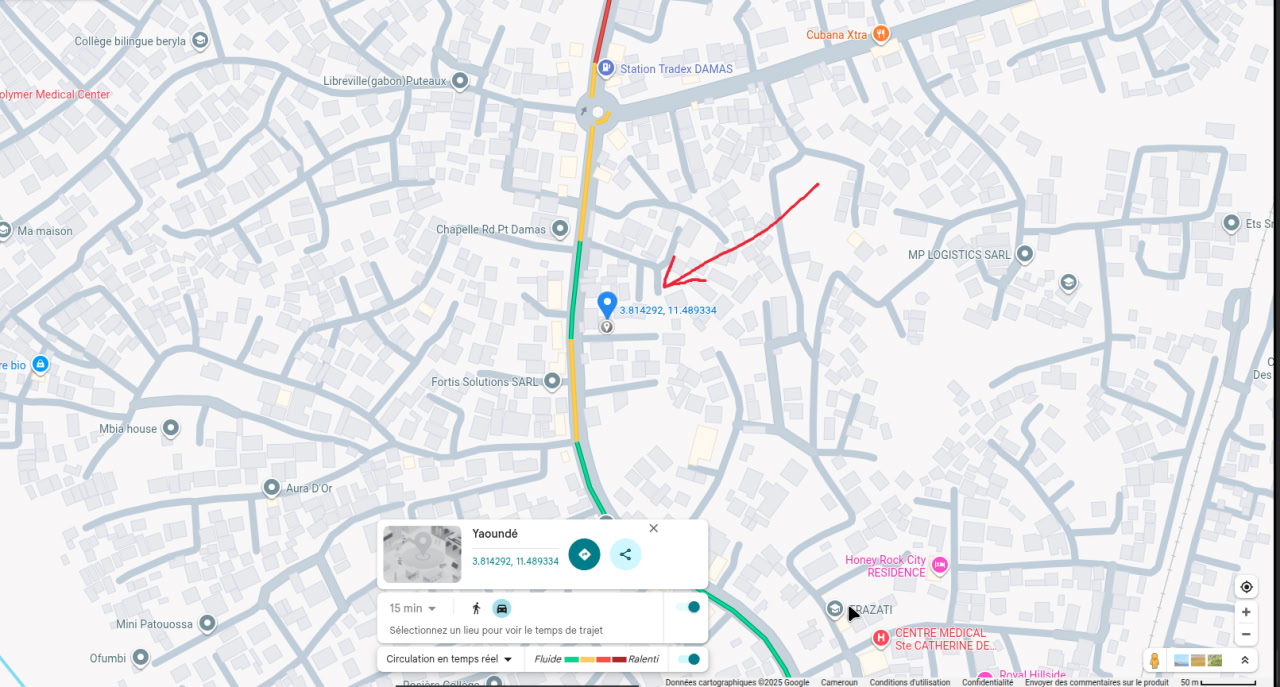
\includegraphics[width=0.68\textwidth, height=6.8cm]{images/localisation.jpg}
    \caption{Localisation géographique de Access Finance \& RH SARL}
    \label{fig:localisation}
\end{figure}

\subsection{Mission et vision}

\textbf{Mission :} Access Finance \& RH SARL analyse les besoins de ses clients, propose des solutions numériques adaptées et pilote leur déploiement dans le respect des délais, de la qualité et des coûts.

\textbf{Vision :} Devenir le partenaire de référence des organisations dans leur transformation numérique et l'optimisation de leurs processus métier.

\subsection{Domaines d'activité}

Access Finance \& RH SARL structure son offre autour de trois axes. Le \textbf{développement d'applications sur mesure} conduit les clients du cahier des charges à la mise en production : applications web, plateformes métier et systèmes d'information adaptés à chaque organisation. Le \textbf{conseil et l'audit numérique} portent sur l'évaluation des systèmes existants et la formulation de recommandations d'optimisation. Enfin, la \textbf{maintenance et le support} garantissent, par contrat, la continuité de service et l'évolution des solutions déployées.

\subsection{Organigramme}

Access Finance \& RH SARL fonctionne avec une structure resserrée, caractéristique des entreprises de services numériques à taille humaine : les circuits de décision sont courts et chaque intervenant couvre un périmètre large. L'organisation s'articule autour des rôles suivants :

\begin{itemize}
    \item \textbf{Direction générale}, assurée par la dirigeante de l'entreprise : orientation stratégique, relation avec les clients institutionnels et arbitrages d'engagement sur les projets.
    \item \textbf{Direction technique (CTO)} : définition des choix d'architecture et de technologies, garantie de la qualité des livrables et encadrement de l'équipe de production.
    \item \textbf{Tech Lead}, chargé du pilotage technique au quotidien : découpage des tâches, revues de code, accompagnement des développeurs et interface avec la direction technique.
    \item \textbf{Équipe de développement} : un développeur senior, référent sur les projets les plus complexes, et les développeurs chargés de l'implémentation des solutions.
    \item \textbf{Design UX/UI} : maquettage des écrans, ergonomie des parcours et cohérence visuelle des interfaces livrées.
    \item \textbf{Équipe commerciale} : prospection, réponse aux consultations et suivi de la relation client.
\end{itemize}

Le présent stage s'est déroulé au sein de l'\textbf{équipe de développement}, sous la supervision de l'encadreur professionnel, avec des points réguliers auprès du Tech Lead pour les choix de conception.

\begin{figure}[H]
    \centering
    \centerline{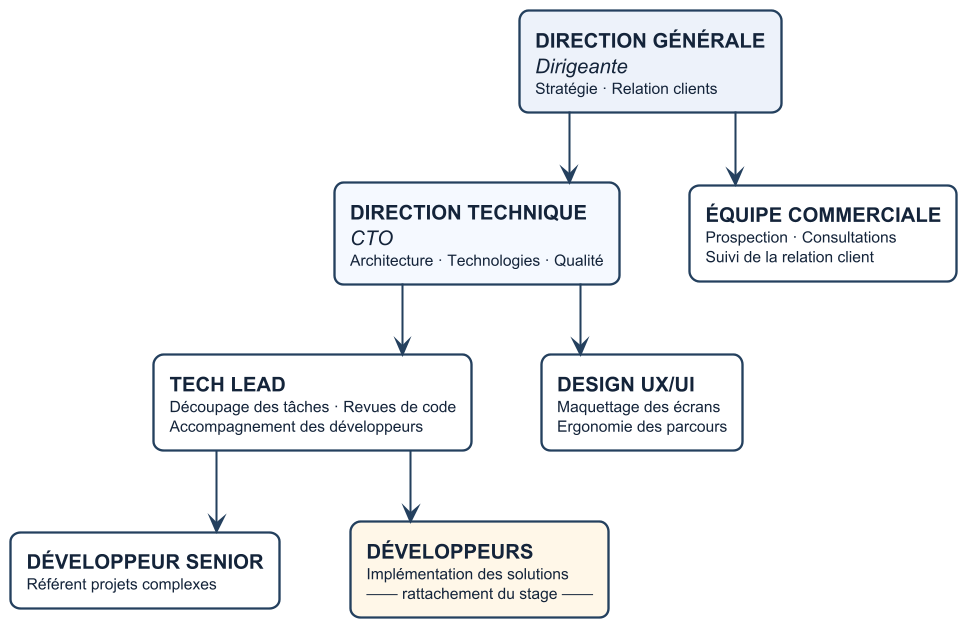
\includegraphics[width=0.80\linewidth]{diagrammes/organigramme_klivar.png}}
    \caption{Organigramme de l'entreprise Access Finance \& RH SARL}
    \label{fig:organigramme}
\end{figure}

\section{Analyse de la situation existante}

Cette section retrace d'abord le déroulement de la mission, puis restitue la procédure de dépôt et de traitement des plaintes telle que l'audit de terrain l'a documentée, avant d'en relever les difficultés.

\subsection{Déroulement du stage et missions effectuées}

Mon intégration au sein de Access Finance \& RH SARL s'est déroulée de manière progressive. Dès les premiers jours, j'ai été présenté aux différents pôles de l'entreprise. Mon maître de stage, M.~\textbf{NDJON MBOG THIERRY}, a encadré l'ensemble de la mission avec rigueur et disponibilité.

La mission s'est déroulée en cinq phases sur les six mois du stage. Les \textbf{deux premières semaines} ont été consacrées à l'audit et à l'analyse de l'existant : observation de la procédure aux commissariats de Ngoa-Ekélé et de Mimboman, entretiens avec les personnels et identification des points de friction. Les \textbf{deux semaines suivantes} ont porté sur la conception de la solution, avec la définition de l'architecture, la modélisation UML et le maquettage des interfaces. Du \textbf{deuxième au quatrième mois} s'est étendu le développement de PlainteCam, couvrant l'implémentation du frontend, celle du backend et l'intégration de l'intelligence artificielle. Le \textbf{cinquième mois} a été réservé aux tests et à la validation : recette fonctionnelle, corrections et validation par les parties prenantes. Le \textbf{sixième et dernier mois} a été employé à la documentation et à la rédaction du présent mémoire.

\subsection{Description de la procédure manuelle actuelle}

L'audit a été conduit dans deux commissariats de Yaoundé, celui de \textbf{Ngoa-Ekélé} et celui de \textbf{Mimboman}, selon une approche qualitative semi-directive : des entretiens avec des fonctionnaires de police de ces unités, menés sur guide structuré et anonymisés pour favoriser la franchise des réponses, complétés par l'observation directe du flux de travail sur place : réception des plaignants, circulation des dossiers papier, gestion des parafeurs. Le recours à deux unités distinctes permettait de distinguer ce qui relève de la procédure commune de ce qui tient aux habitudes propres à un service. La procédure reconstituée ci-dessous s'articule en quatre temps.

\subsubsection*{Réception et enregistrement}

Le plaignant se présente au commissariat \textbf{territorialement compétent}, c'est-à-dire celui du secteur où réside le mis en cause ou celui où les faits ont eu lieu, le maillage des unités étant fixé par l'organisation de la Sûreté nationale. Sa plainte doit obligatoirement comporter la date, ses nom et adresse, l'objet de la plainte, l'identité du mis en cause et la destination de l'acte, commissaire ou procureur. Le secrétariat enregistre la plainte et la transmet au chef d'unité. Une \textbf{attestation de dépôt} est délivrée au plaignant et jointe au dossier : elle constitue la preuve officielle qu'il a bien porté plainte.

\subsubsection*{Cotation à un enquêteur}

Le chef d'unité \textbf{cote} ensuite la plainte à un enquêteur, lequel reçoit un \textbf{parafeur} regroupant l'ensemble des dossiers dont il a la charge. Le critère retenu est la compétence de l'enquêteur sur le type d'affaire concerné, mais \textbf{aucune procédure n'est formalisée} : l'arbitrage repose sur la connaissance qu'a le chef d'unité de son équipe. En cas d'indisponibilité de l'enquêteur désigné, le dossier est transféré à un autre.

\subsubsection*{Auditions et procès-verbaux}

Le plaignant est convoqué puis auditionné, et un \textbf{procès-verbal} est dressé. Le mis en cause est convoqué à son tour et auditionné, donnant lieu à un second procès-verbal. Lorsqu'il est identifié, il est convoqué \textbf{au minimum trois fois} ; en cas d'absence répétée et injustifiée, le dossier est transmis au procureur.

La rédaction des procès-verbaux est \textbf{entièrement manuscrite}. L'enquêteur transcrit à la main les déclarations en suivant un \textbf{template institutionnel} normalisé : en-tête (commissariat, date, heure, numéro de dossier), identité complète de la personne auditionnée, corps de la déclaration, questions et réponses le cas échéant, clôture et mentions légales.

\subsubsection*{Convocation et suivi}

Un point particulier est apparu déterminant lors de l'entretien : c'est \textbf{en principe le plaignant lui-même qui remet la convocation au mis en cause}. Un policier ne l'assiste que s'il redoute des représailles. Quant au suivi, il n'existe \textbf{aucun dispositif} : pour connaître l'état d'avancement de son dossier, le plaignant doit se déplacer au commissariat.

\begin{figure}[H]
    \centering
    
\includegraphics[width=0.72\textwidth]{images/problematique_flux.png}
    \caption{Flux de traitement manuel : points de friction identifiés}
    \label{fig:flux_manuel}
\end{figure}

Cette procédure ne laisse \textbf{aucune trace numérique}. Il en découle une conséquence que l'audit a jugée centrale : le délai qui sépare le dépôt de la cotation, comme celui du traitement complet d'une affaire, \textbf{n'est mesuré nulle part}. Il varie selon l'affluence, la nature des faits et la disponibilité des enquêteurs, et seul le commissariat en a une appréciation empirique. Ce n'est donc pas la longueur des délais qui constitue le problème documenté, mais l'\textbf{impossibilité de les connaître}, et par conséquent de les piloter.

\subsection{Difficultés et limites identifiées lors de l'audit}

L'entretien a permis de recenser quatre difficultés récurrentes, qui tiennent moins à l'organisation du service qu'aux situations concrètes rencontrées au guichet et en salle d'audition.

La première tient à l'\textbf{analphabétisme d'une partie des plaignants}, qui ne savent ni lire ni écrire et doivent être assistés par une personne de leur choix. La procédure s'en trouve ralentie, le plaignant devient dépendant d'un tiers, et la confidentialité de sa déclaration s'en trouve fragilisée.

La deuxième tient à la \textbf{difficulté d'exposer les faits de façon claire et ordonnée}. Beaucoup de plaignants racontent par fragments, dans le désordre, en omettant des éléments qu'ils jugent secondaires. Il en résulte un dossier incomplet et un procès-verbal lacunaire.

La troisième, et l'entretien l'a présentée comme la plus contentieuse, est le \textbf{refus du mis en cause de signer le procès-verbal} dont il conteste la fidélité. Elle ouvre un contentieux procédural et fait peser un risque de vice de forme sur la suite de l'affaire.

La quatrième tient à la \textbf{rédaction manuscrite des procès-verbaux}, longue et répétitive. Elle représente une charge administrative lourde, et ce temps est directement soustrait au travail d'enquête proprement dit.

À ces difficultés s'ajoutent trois limites structurelles relevées par l'observation : le \textbf{déplacement obligatoire} pour déposer comme pour s'informer, l'\textbf{absence de traçabilité} interdisant tout audit et toute mesure, et la \textbf{remise de la convocation par le plaignant lui-même}, qui fait peser sur la victime une démarche potentiellement risquée.

Il est notable que trois de ces quatre difficultés, les points 1 à 3, concernent la \textbf{qualité et la valeur juridique de la déclaration} plutôt que la lenteur du circuit. Ce constat a orienté la conception : la solution devait d'abord fiabiliser le recueil des faits, et non se contenter d'accélérer la circulation des dossiers.

\section{Ce qui existe ailleurs}

Avant d'envisager un développement, il fallait vérifier qu'aucune solution existante ne répondait déjà au besoin. Trois dispositifs comparables ont été examinés.

En \textbf{France}, le dispositif de pré-plainte a laissé place, en octobre 2024, à une \textbf{plainte en ligne} de plein exercice, doublée d'un service de visioconférence dénommé \textit{Visioplainte}~\cite{france-visioplainte}. Le plaignant y dépose sa plainte sans se déplacer, s'entretient à distance avec un officier, puis reçoit le procès-verbal par voie électronique et le confirme avant signature par l'agent. Ce dispositif demeure toutefois réservé aux \textbf{atteintes aux biens dont l'auteur est inconnu} : les faits commis contre les personnes, comme ceux dont l'auteur est identifié, en restent exclus, au motif qu'ils peuvent justifier une intervention immédiate.

Au \textbf{Sénégal}, la police nationale a mis en service en février 2026 une \textbf{plateforme de signalement des infractions cybercriminelles}~\cite{senegal-psic}. Elle permet de dénoncer en ligne, de manière sécurisée et confidentielle, les escroqueries commises sur internet, le cyberharcèlement, l'usurpation d'identité ou les atteintes aux données personnelles. Son périmètre est donc \textbf{thématique} : il ne couvre que la délinquance numérique, et le dispositif s'arrête au signalement, sans prendre en charge l'instruction qui doit suivre.

Au \textbf{Cameroun} enfin, la Délégation générale à la sûreté nationale a engagé en 2022, avec l'appui de la coopération allemande, un projet de plateforme numérique destinée au traitement automatisé des plaintes des usagers~\cite{cameroun-dgsngiz}. Son objet est cependant \textbf{distinct du nôtre} : il s'agit de recueillir les plaintes \emph{dirigées contre la police}, dans une logique de contrôle interne, et non de permettre à une victime de déposer une plainte pénale. Le numéro vert qui remplissait auparavant cette fonction était du reste jugé peu efficace par le public.

Deux enseignements se dégagent de cette comparaison. D'abord, les dispositifs existants sont \textbf{restreints} : soit par la nature des faits (atteintes aux biens, cyberinfractions), soit par la qualité de l'auteur, qui doit demeurer inconnu. Ensuite, ils s'arrêtent au \textbf{dépôt} ou au signalement : aucun ne prend en charge la suite de la chaîne, c'est-à-dire la cotation à un enquêteur, la conduite des auditions, la rédaction des procès-verbaux et l'émission des convocations.

Aucun de ces dispositifs ne traite les difficultés relevées lors de notre audit : un plaignant qui ne sait ni lire ni écrire, une convocation remise par la victime elle-même, une cotation sans procédure formalisée. Ces constats justifient le développement d'une solution propre plutôt que la reprise d'un outil existant.

Le dispositif français mérite toutefois d'être retenu comme \textbf{piste d'évolution} : en faisant dialoguer la victime avec un officier par visioconférence, il apporte au problème de l'illettrisme une réponse que PlainteCam traite autrement, par la dictée vocale et le questionnaire guidé. Les deux approches sont complémentaires plutôt que concurrentes.

\section{Analyse SWOT liée à la mission}

Le service observé ne part pas de rien. Ses \textbf{forces} ne sont d'ailleurs ni techniques ni matérielles : elles sont humaines et juridiques. Il dispose de personnels formés, rompus à la conduite des auditions et à la qualification juridique des faits ; d'une connaissance fine du terrain, que les entretiens menés dans les deux commissariats ont confirmée ; d'un maillage territorial d'unités déjà établi et connu des habitants ; enfin d'un cadre de procédure stable, qui désigne sans ambiguïté qui peut dresser un procès-verbal et dans quelles formes.

Ses \textbf{faiblesses} tiennent au support de la procédure, non aux personnes qui l'appliquent. Le dossier circule sur papier, aucun système d'information ne le suit, et l'absence de trace numérique interdit non seulement l'audit mais toute mesure : ni le délai de cotation ni celui du traitement complet ne sont connus. La hiérarchie ne dispose donc d'aucun élément objectif pour répartir la charge entre ses enquêteurs, ni pour rendre compte de l'activité de son unité.

Deux évolutions extérieures constituent aujourd'hui des \textbf{opportunités} qui n'existaient pas hier : la maturité des technologies web, qui permet de livrer un service utilisable depuis un terminal modeste et une connexion instable, et l'accessibilité de l'intelligence artificielle générative, dont certains modèles s'obtiennent désormais sans engagement financier. S'y ajoute le taux d'équipement mobile des citoyens, sans lequel un dépôt en ligne resterait une hypothèse d'école.

Les \textbf{menaces} sont de deux ordres. Les premières pèsent sur le service tel qu'il fonctionne : la perte de confiance de citoyens lassés de se déplacer sans obtenir d'information, et l'égarement ou l'altération de dossiers que rien ne duplique. Les secondes naîtraient du projet lui-même : la résistance au changement de personnels attachés à des pratiques éprouvées, et surtout la contestation de la valeur probante d'un dossier constitué par voie numérique.

C'est le \textbf{croisement} de ces facteurs qui a orienté la conception, davantage que leur inventaire. Le cadre juridique stable, porté au rang des forces, est précisément ce qui désarme la menace la plus sérieuse : un dossier numérique demeure défendable tant que le procès-verbal reste l'acte de l'officier de police judiciaire, ce qui exclut toute validation automatique. La faiblesse la plus lourde, des délais que personne ne mesure, trouve dans la maturité des technologies web une réponse immédiate, l'horodatage de chaque transition. Quant au maillage territorial, il cesse d'être un simple actif pour devenir le socle du rattachement automatique au commissariat compétent : la cascade géographique ne fait que rendre calculable une organisation déjà en place.

\section{Identification du besoin}

Les constats qui précèdent convergent vers une même conclusion, qu'il reste à formuler explicitement avant d'aborder la conception.

\subsection{Pourquoi les méthodes actuelles ne suffisent plus}

L'analyse de l'existant a mis en évidence quatre problèmes fondamentaux qui rendent la procédure actuelle insuffisante :

\textbf{Un problème d'accessibilité :} Le déplacement au commissariat constitue une barrière significative, en particulier pour les personnes éloignées, à mobilité réduite ou craignant de se présenter en personne. Il réduit le nombre de plaintes effectivement déposées et alourdit inutilement le parcours du citoyen.

\textbf{Un problème de fiabilité du recueil :} La qualité du dossier dépend de la capacité du plaignant à exposer les faits et de la retranscription qu'en fait l'agent. Un plaignant illettré, intimidé ou peu à l'aise à l'oral produit une déclaration lacunaire, que la rédaction manuscrite du procès-verbal ne permet ni de compléter ni de contrôler méthodiquement.

\textbf{Un problème de sécurité pour le plaignant :} La remise de la convocation au mis en cause incombe en principe à la victime elle-même. Cette exposition directe, dans une affaire où l'auteur présumé est souvent un proche ou un voisin, peut dissuader de poursuivre la procédure, voire de la déclencher.

\textbf{Un problème de traçabilité :} L'absence de système d'information centralisé empêche tout suivi par le plaignant, tout audit a posteriori et toute mesure de l'activité du service. Faute d'horodatage, le commissariat ne dispose d'aucun élément objectif pour arbitrer l'affectation de ses moyens ni pour rendre compte de son activité.

Trois contraintes encadrent la réponse à apporter. La première est juridique : le procès-verbal demeure un acte de l'officier de police judiciaire, et aucun dispositif automatique ne peut s'y substituer~\cite{cameroun-cpp}. La deuxième tient à la confidentialité : un dossier de plainte n'est consultable que par son plaignant, l'enquêteur qui en a la charge et sa hiérarchie. La troisième est matérielle : la plateforme doit rester utilisable depuis un terminal mobile d'entrée de gamme et une connexion instable.

Enfin, une réserve de périmètre doit être posée d'emblée : la contestation par le mis en cause du contenu de son procès-verbal relève de la procédure, non du logiciel. La plateforme peut en conserver la trace horodatée, elle ne peut pas l'empêcher. Il ne sera donc pas prétendu qu'elle résout cette difficulté.
   % Chapitre 1
% CHAPITRE 2 — Conception de la plateforme PlainteCam

\chapter{Conception de la plateforme PlainteCam}
\label{ch:conception}

Le chapitre précédent a établi ce que la procédure manuelle ne permet pas de faire. Le présent chapitre répond à la question inverse : que doit faire la plateforme, et comment doit-elle être organisée pour le faire ?

Il progresse du besoin vers la structure. La première section décrit les fonctionnalités attendues, les cas d'utilisation majeurs, puis les besoins fonctionnels et non fonctionnels qui en découlent, avant de les formaliser dans un diagramme de cas d'utilisation. La deuxième expose la démarche retenue pour conduire le projet. La troisième présente l'architecture de la solution, d'abord sous son angle fonctionnel puis sous son angle modulaire. La quatrième complète cette vue par la modélisation UML des données et des échanges.

Aucun outil ni aucune technologie n'est nommé dans ce chapitre : la conception y est tenue indépendante des moyens de sa réalisation, de sorte qu'elle reste valable si ces moyens changent. Le choix des technologies et la mise en œuvre effective font l'objet du chapitre~\ref{ch:realisation}.

\section{Conception fonctionnelle}

Concevoir la plateforme suppose d'abord de dire ce qu'elle fait, pour qui et sous quelles contraintes. Cette section procède en quatre temps : l'inventaire des fonctionnalités, les cas d'utilisation qui les mobilisent, les besoins fonctionnels qui en découlent, et leur formalisation graphique.

\subsection{Description des fonctionnalités}

PlainteCam s'organise en quatre espaces, un par profil d'utilisateur. Chacun ne donne accès qu'aux fonctions relevant de son rôle, ce cloisonnement étant une exigence et non une commodité : un plaignant ne doit en aucun cas apercevoir le dossier d'un autre.

L'\textbf{espace citoyen} permet au plaignant de déposer sa plainte au terme d'un parcours guidé en cinq écrans, d'y joindre les pièces dont il dispose, de télécharger son récépissé et de suivre en ligne l'avancement de son dossier sans se déplacer. Pendant la rédaction des faits, un indicateur de complétude lui signale les éléments encore absents de sa déclaration.

L'\textbf{espace commissaire} donne au chef d'unité la vue d'ensemble dont la procédure papier le privait. Il y cote les dossiers entrants à un enquêteur en fixant leur priorité, consulte le tableau de bord et les statistiques de son commissariat, gère les comptes de ses agents et accède au journal d'audit.

L'\textbf{espace enquêteur} regroupe les actes d'instruction. L'enquêteur y consulte les dossiers qui lui ont été cotés, consigne les auditions, obtient une proposition de procès-verbal qu'il révise et valide, émet les convocations et fait progresser le statut du dossier jusqu'à sa clôture.

L'\textbf{espace administrateur} se limite à l'administration technique : création et désactivation des comptes, tenue du référentiel des commissariats et de leur ressort territorial. Il n'ouvre aucun accès au contenu des plaintes.

\subsection{Cas d'utilisation majeurs}

Quatre cas d'utilisation structurent le fonctionnement de la plateforme. Ils correspondent aux quatre moments où un acteur agit sur le dossier et en modifie l'état.

Le \textbf{dépôt d'une plainte} est le point d'entrée. Le plaignant déclare la nature de l'infraction et le lieu des faits, à partir duquel la plateforme détermine le commissariat territorialement compétent. Il rédige ensuite son récit, renseigne l'identité du mis en cause lorsqu'elle est connue, répond aux questions complémentaires que la plateforme lui pose, puis signe et confirme. Un récépissé numéroté lui est délivré immédiatement.

La \textbf{cotation d'un dossier} est l'acte du commissaire. Il examine les plaintes reçues par son unité, désigne l'enquêteur chargé de l'affaire et fixe la priorité du dossier. Cette opération fait basculer le dossier de l'attente vers l'instruction et déclenche la notification de l'enquêteur.

L'\textbf{instruction d'un dossier} couvre le travail de l'enquêteur. Il convoque les parties, tient les auditions et en dresse les procès-verbaux, en s'appuyant sur une proposition rédigée automatiquement à partir de la déclaration du plaignant. Il reste seul responsable du contenu : rien n'est enregistré sans sa validation explicite.

Le \textbf{suivi du dossier} est le cas d'utilisation transverse. Le plaignant consulte à tout moment l'état de sa procédure depuis son espace, tandis que le commissaire en suit l'avancement consolidé sur son tableau de bord. Ce suivi n'existait sous aucune forme dans la procédure papier.

\subsection{Besoins fonctionnels}

De ces cas d'utilisation découlent les besoins fonctionnels que la plateforme doit satisfaire, c'est-à-dire les services qu'elle doit rendre. Ils sont énumérés ci-dessous et serviront de référence à la recette présentée au chapitre~\ref{ch:realisation}.

\begin{itemize}
    \item \textbf{BF1. Dépôt en ligne.} Permettre le dépôt intégral d'une plainte sans déplacement au commissariat, au terme d'un parcours compréhensible par un public non juriste.
    \item \textbf{BF2. Rattachement territorial automatique.} Déterminer le commissariat compétent à partir du lieu des faits, sans que le plaignant ait à le connaître.
    \item \textbf{BF3. Assistance à la déclaration.} Signaler au plaignant les éléments manquants de son récit et lui poser les questions complémentaires propres à la nature d'infraction déclarée.
    \item \textbf{BF4. Cotation.} Permettre au commissaire de désigner un enquêteur et de fixer une priorité, et notifier l'agent désigné.
    \item \textbf{BF5. Rédaction assistée du procès-verbal.} Produire une proposition de procès-verbal à partir de la déclaration, systématiquement soumise à la révision et à la validation de l'enquêteur.
    \item \textbf{BF6. Suivi par le plaignant.} Rendre l'état d'avancement du dossier consultable en ligne à tout moment, et notifier chaque changement de statut.
    \item \textbf{BF7. Production des pièces.} Générer le récépissé, les procès-verbaux et les convocations au format imprimable, munis d'un identifiant vérifiable.
    \item \textbf{BF8. Pilotage.} Fournir au commissaire des indicateurs consolidés sur le volume, la répartition et la charge des enquêteurs de son ressort.
\end{itemize}

\subsection{Besoins non fonctionnels}

Les besoins précédents disent ce que la plateforme doit faire. Ceux qui suivent disent sous quelles conditions elle doit le faire, et ils pèsent ici plus lourd que dans une application ordinaire : une plainte est un acte de procédure, dont la valeur dépend autant de la manière dont il est conservé que de son contenu.

\begin{itemize}
    \item \textbf{BNF1. Confidentialité et cloisonnement.} Restreindre la visibilité des dossiers selon le rôle : le plaignant aux siens, l'enquêteur à ceux qui lui sont cotés, le commissaire à ceux de son unité. Le cloisonnement doit résister à une requête mal formée, et pas seulement aux parcours prévus par l'interface.
    \item \textbf{BNF2. Traçabilité et auditabilité.} Horodater chaque acte de procédure et le rattacher à son auteur dans un journal consultable et non modifiable, y compris par un administrateur. C'est la condition pour reconstituer une procédure a posteriori.
    \item \textbf{BNF3. Intégrité et valeur probante.} Garantir qu'aucune pièce produite ne puisse être altérée après signature, et qu'un procès-verbal ne soit jamais enregistré sans validation explicite de l'officier de police judiciaire, seul habilité à le dresser.
    \item \textbf{BNF4. Accessibilité.} Rester utilisable par un plaignant sans culture juridique ni aisance informatique. Le vocabulaire des écrans doit éviter les termes de procédure, et le parcours doit tolérer qu'une tierce personne assiste un plaignant qui ne sait ni lire ni écrire.
    \item \textbf{BNF5. Temps de réponse.} Maintenir un délai d'affichage compatible avec les connexions disponibles localement, et borner l'attente de la proposition de procès-verbal, dont la génération dépend d'un service externe.
    \item \textbf{BNF6. Portabilité.} Fonctionner sur les navigateurs courants, sur poste comme sur téléphone, sans installation préalable : le plaignant ne doit rien avoir à installer pour déposer.
    \item \textbf{BNF7. Maintenabilité.} Isoler les éléments appelés à changer, en particulier le référentiel des commissariats et les libellés des pièces, afin qu'une évolution du maillage territorial ou de la réglementation n'impose pas de reprendre le code.
\end{itemize}

La suite du chapitre décrit les conceptions retenues pour couvrir ces deux séries de besoins.

\subsection{Diagramme de cas d'utilisation}

La figure~\ref{fig:usecase} formalise ces cas d'utilisation et les répartit entre \textbf{quatre acteurs}. Le \textbf{plaignant} dépose sa plainte, suit l'avancement de son dossier et télécharge son récépissé. Le \textbf{commissaire} cote les dossiers entrants, consulte le tableau de bord de son unité, gère ses agents et accède au journal d'audit. L'\textbf{enquêteur} instruit les dossiers qui lui sont cotés, émet les convocations, dresse les procès-verbaux et fait progresser le statut. L'\textbf{administrateur} n'intervient que sur les comptes et le référentiel des commissariats.

\begin{figure}[H]
    \centering
    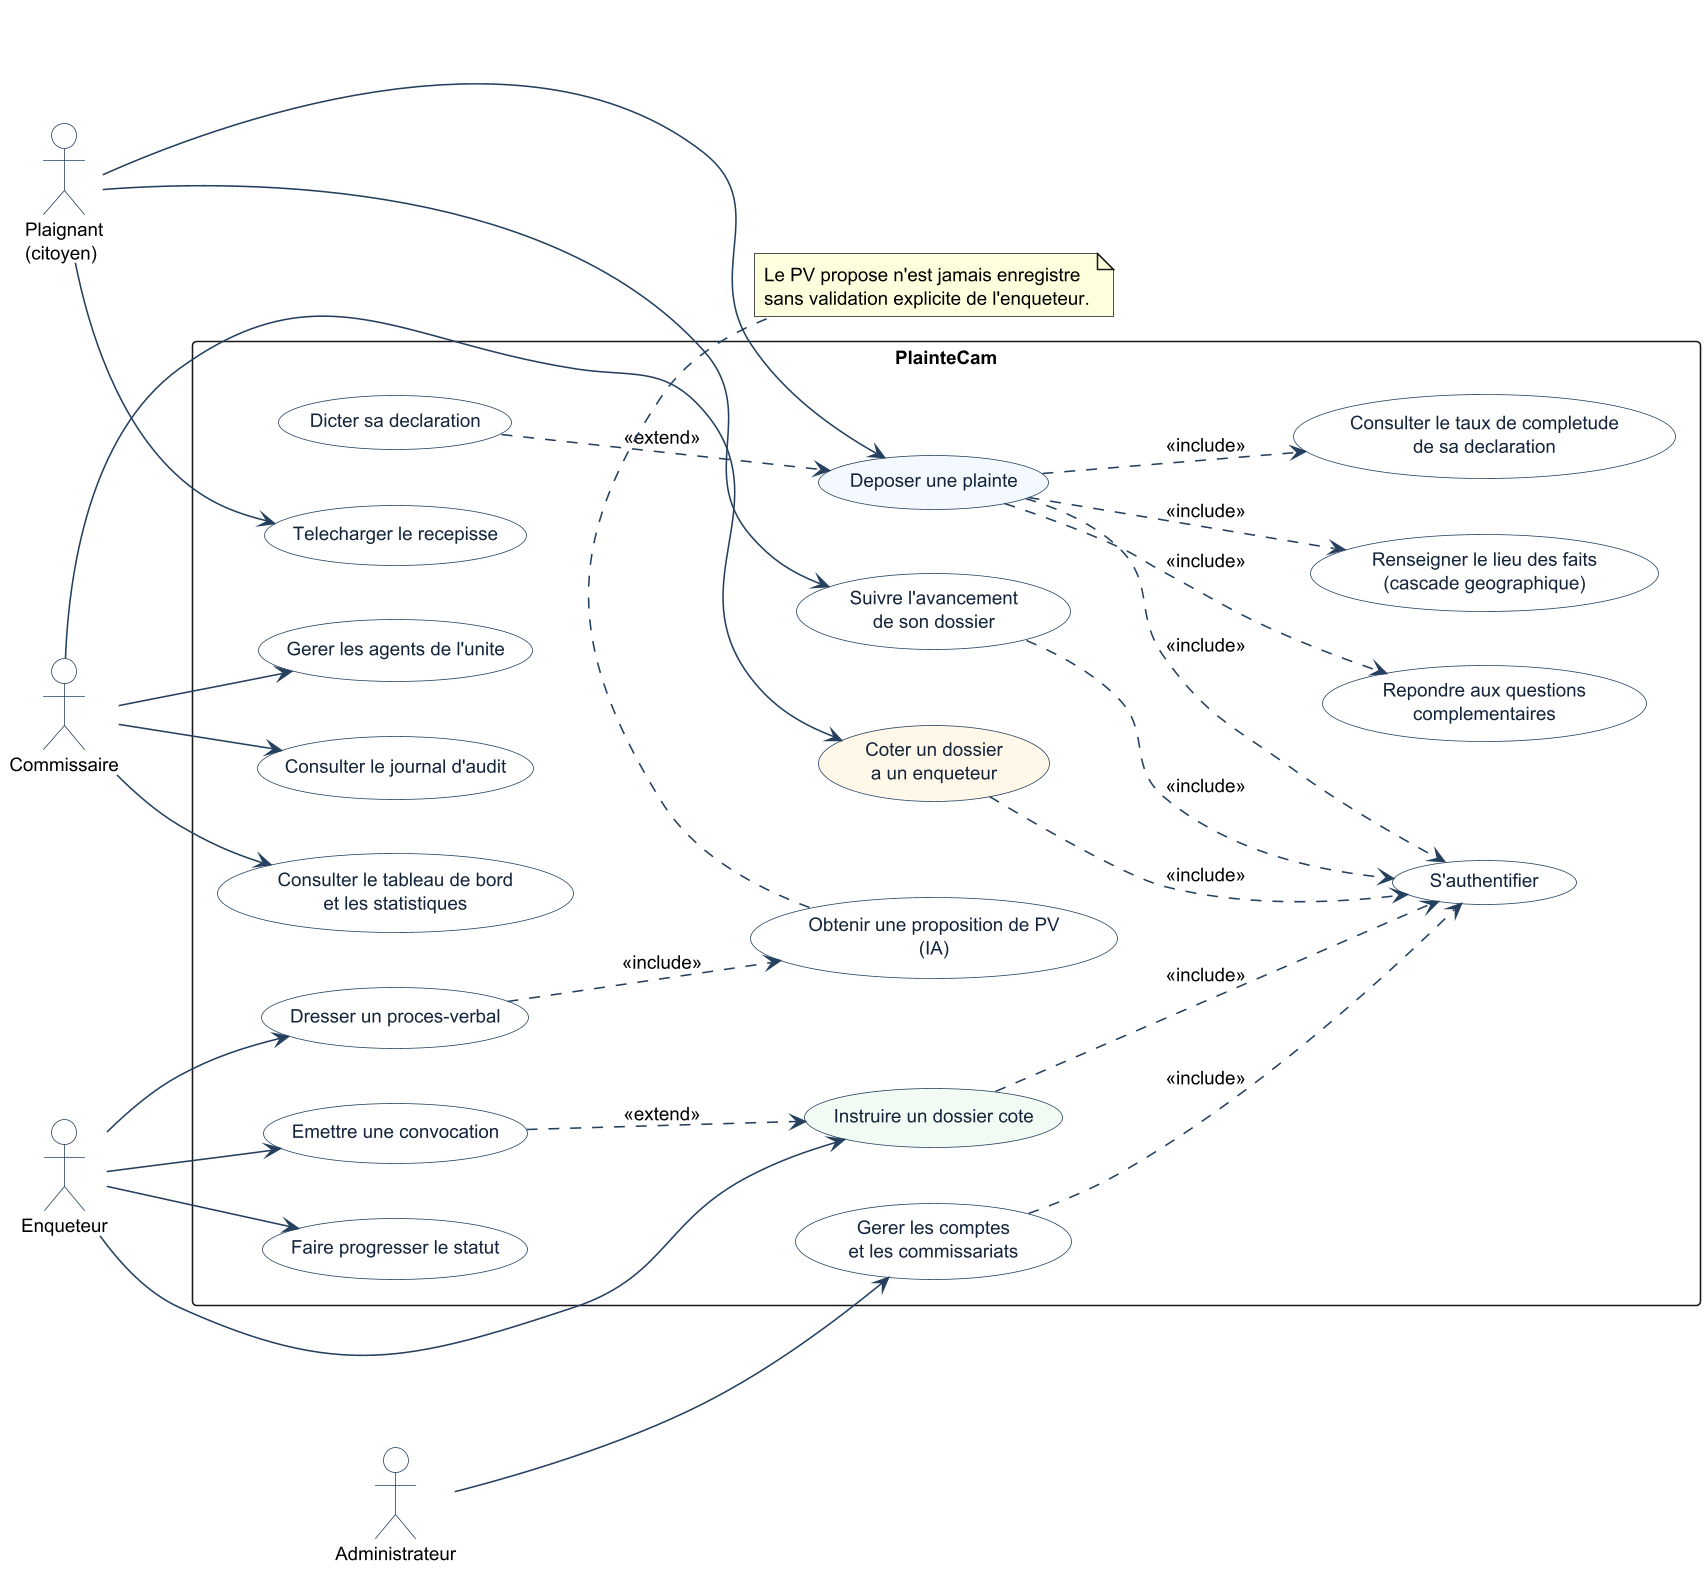
\includegraphics[width=\linewidth]{diagrammes/usecase.png}
    \caption{Diagramme de cas d'utilisation de PlainteCam}
    \label{fig:usecase}
\end{figure}

Deux relations méritent l'attention, car elles portent des règles métier et non de simples commodités d'écriture. La cascade géographique, le calcul du taux de complétude et les questions complémentaires sont des cas \textbf{inclus} dans « déposer une plainte » : ils ne s'exécutent jamais séparément, et le dépôt ne peut aboutir sans eux. De la même façon, « obtenir une proposition de procès-verbal » est inclus dans « dresser un procès-verbal », et non offert comme cas autonome. Le modèle traduit ainsi le principe selon lequel l'intelligence artificielle n'intervient qu'à l'intérieur d'un acte dont l'enquêteur reste responsable. Seule la dictée vocale constitue une \textbf{extension} : elle enrichit le dépôt sans lui être nécessaire.

\section{Démarche adoptée}

Les besoins étant posés, reste à décrire la manière dont le projet a été conduit pour y répondre.

\subsection{Méthodologie de gestion de projet : Agile / Scrum}

Face à la complexité et à l'évolutivité du projet, la méthodologie \textbf{Agile Scrum}~\cite{agile-manifesto} a été adoptée. Cette approche itérative et incrémentale permet de livrer des fonctionnalités en continu, de s'adapter aux retours des parties prenantes et de maîtriser les risques tout au long du développement. Six sprints de trois à quatre semaines ont structuré les six mois de mission.

Le premier sprint a posé les fondations : authentification par jeton, gestion des profils et navigation par rôle. Le deuxième a livré le dépôt de plainte, avec son formulaire en cinq étapes, sa cascade géographique et ses pièces jointes. Le troisième a introduit l'assistance à la déclaration, c'est-à-dire les questions complémentaires, la dictée vocale et la rédaction assistée du procès-verbal. Le quatrième a ouvert l'espace enquêteur, avec les procès-verbaux d'audition et les convocations. Le cinquième a construit l'espace commissaire, sa cotation, ses statistiques et le suivi offert au plaignant. Le sixième et dernier sprint a été consacré à la consolidation : journal d'audit, production des pièces PDF, recette et corrections.

\section{Architecture de la solution}

L'architecture de PlainteCam est présentée sous deux angles complémentaires : ce que la plateforme fait, puis comment elle se découpe en modules. La traduction de ces modules en technologies est traitée au chapitre suivant, car elle relève de la réalisation et non de la conception.

\subsection{Architecture fonctionnelle}

La figure~\ref{fig:archi_fonctionnelle} donne la vue d'ensemble des fonctions de la plateforme. Le cycle de vie d'une plainte s'y lit de gauche à droite en cinq temps, chacun rattaché à l'acteur qui en a la charge : le plaignant \textbf{dépose} sa déclaration, la plateforme \textbf{oriente} le dossier vers le commissariat territorialement compétent, le commissaire le \textbf{cote} à un enquêteur, celui-ci \textbf{instruit} l'affaire puis la \textbf{clôture}.

\begin{figure}[H]
    \centering
    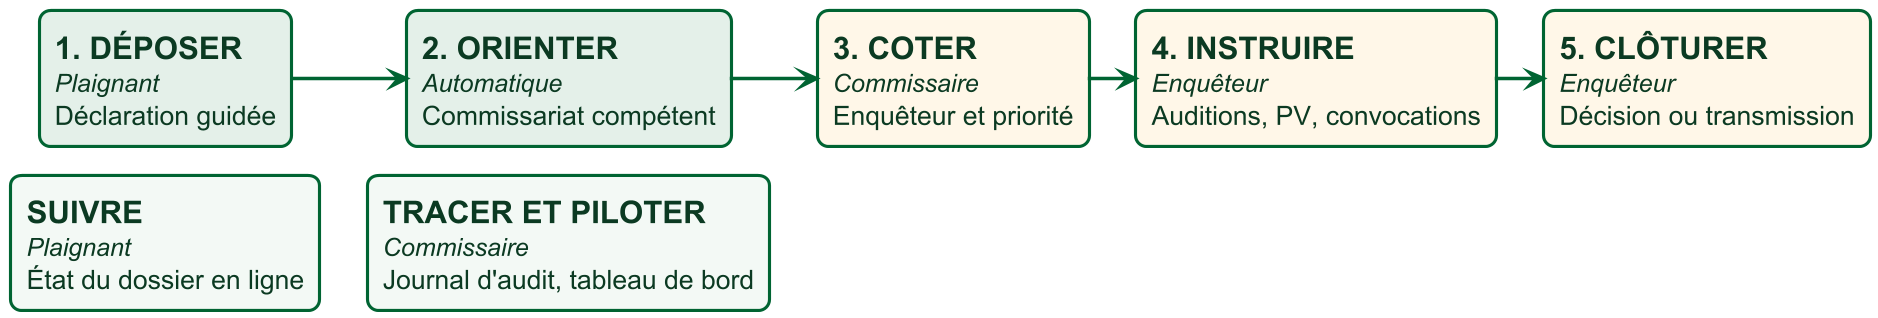
\includegraphics[width=\linewidth]{diagrammes/architecture_fonctionnelle.png}
    \caption{Architecture fonctionnelle : les grandes fonctions de PlainteCam}
    \label{fig:archi_fonctionnelle}
\end{figure}

Deux fonctions échappent à cette séquence parce qu'elles la traversent de bout en bout. Le \textbf{suivi} rend chaque transition visible du plaignant, sans qu'il ait à se déplacer. La \textbf{traçabilité} inscrit ces mêmes transitions au journal d'audit et alimente le tableau de bord du commissaire. Elles ne constituent pas une étape du cycle mais une propriété de l'ensemble, et c'est à ce titre qu'elles figurent à part sur le schéma.

\subsection{Architecture de conception}

La figure~\ref{fig:archi_conception} décompose la solution en modules, indépendamment de toute technologie. Trois ensembles se dégagent autour d'un noyau.

\begin{figure}[H]
    \centering
    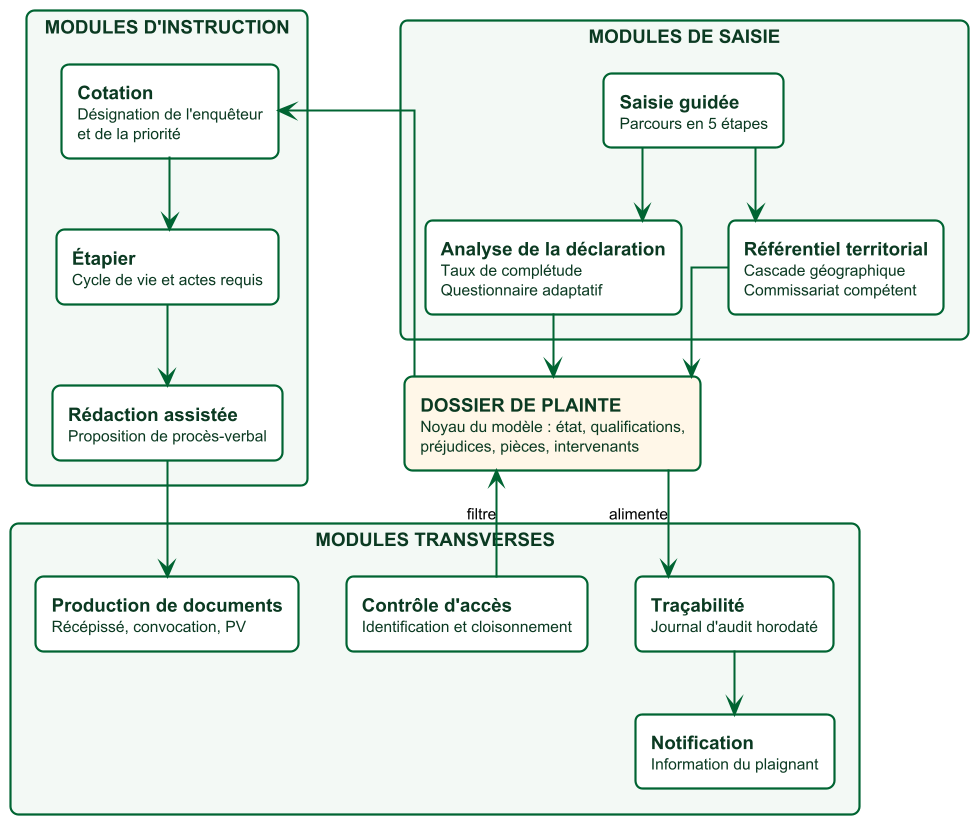
\includegraphics[width=0.86\linewidth]{diagrammes/architecture_conception.png}
    \caption{Architecture de conception : modules et connexions}
    \label{fig:archi_conception}
\end{figure}

Les \textbf{modules de saisie} recueillent la déclaration : le parcours guidé, l'analyse qui en déduit le taux de complétude et les questions à poser, et le référentiel territorial qui détermine l'unité compétente. Les \textbf{modules d'instruction} prennent le relais après le dépôt, avec la cotation, l'étapier qui contraint le cycle de vie, et la rédaction assistée du procès-verbal. Les \textbf{modules transverses} servent les deux précédents : contrôle d'accès, production des documents, traçabilité et notification.

Au centre, le \textbf{dossier de plainte} concentre l'état, les qualifications, les préjudices, les pièces et les intervenants. Tous les modules s'y rattachent, aucun ne dialogue directement avec un autre groupe. Ce choix évite qu'une évolution du parcours de saisie n'affecte l'instruction, et réciproquement.

\section{Modélisation UML}

Les deux diagrammes qui suivent précisent la conception en descendant d'un niveau : le premier décrit les entités manipulées, le second l'enchaînement des échanges entre acteurs et composants.

\subsection{Diagramme de classes}

Le diagramme de classes constitue l'élément central de la modélisation orientée objet. Il décrit comment les entités du domaine interagissent pour concrétiser les différents cas d'utilisation.

\begin{figure}[H]
    \centering
    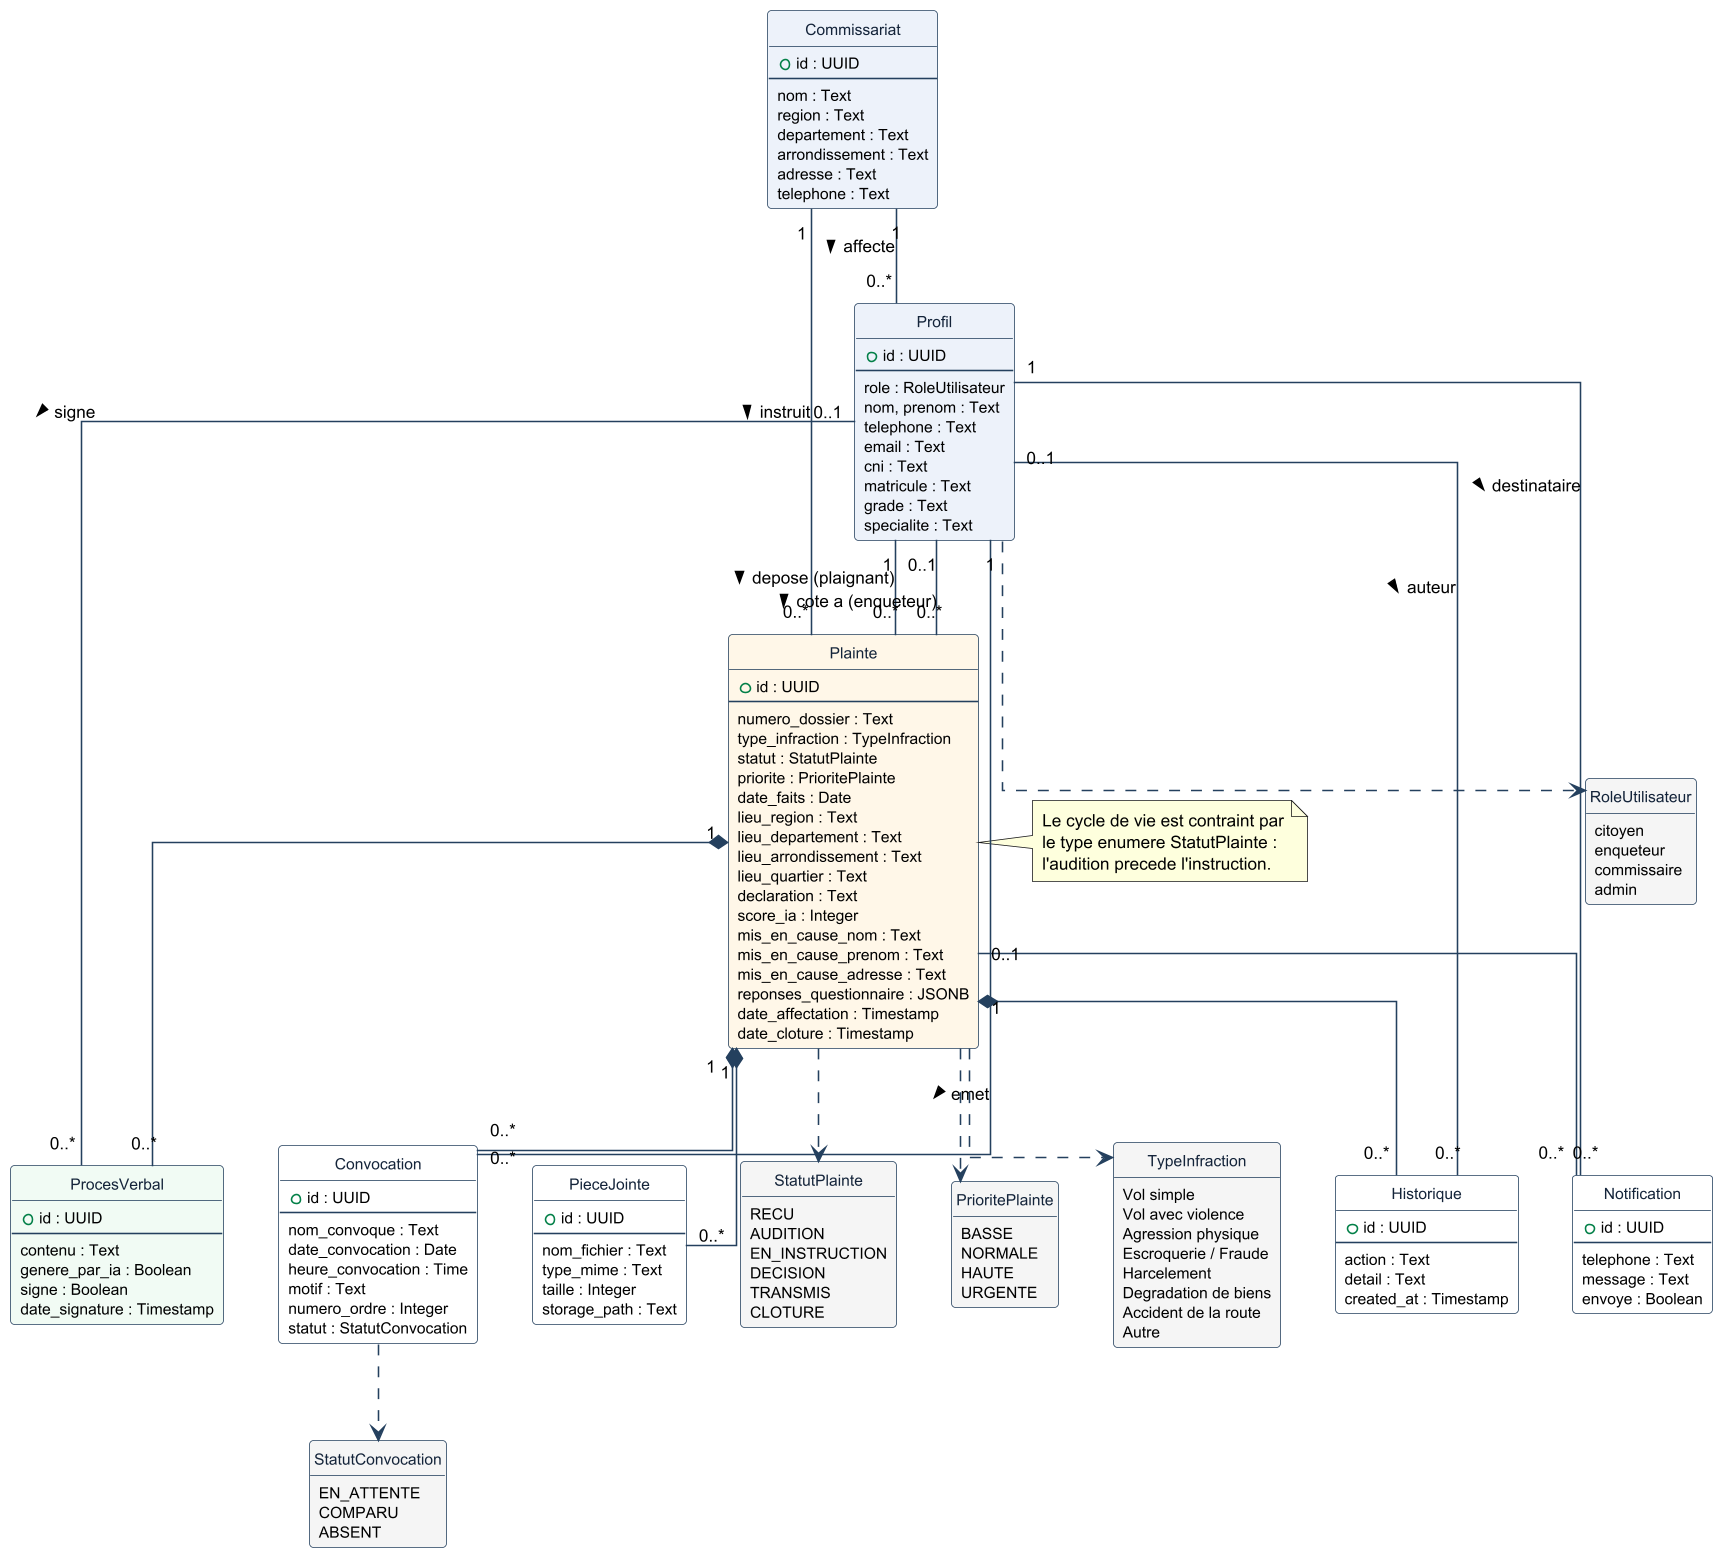
\includegraphics[width=\linewidth]{diagrammes/classe.png}
    \caption{Diagramme de classes : modèle conceptuel de PlainteCam}
    \label{fig:classe}
\end{figure}

\subsection{Diagramme de séquence}

La figure~\ref{fig:sequence} illustre la séquence du dépôt d'une plainte, depuis la saisie guidée jusqu'à la rédaction assistée du procès-verbal.

\begin{figure}[H]
    \centering
    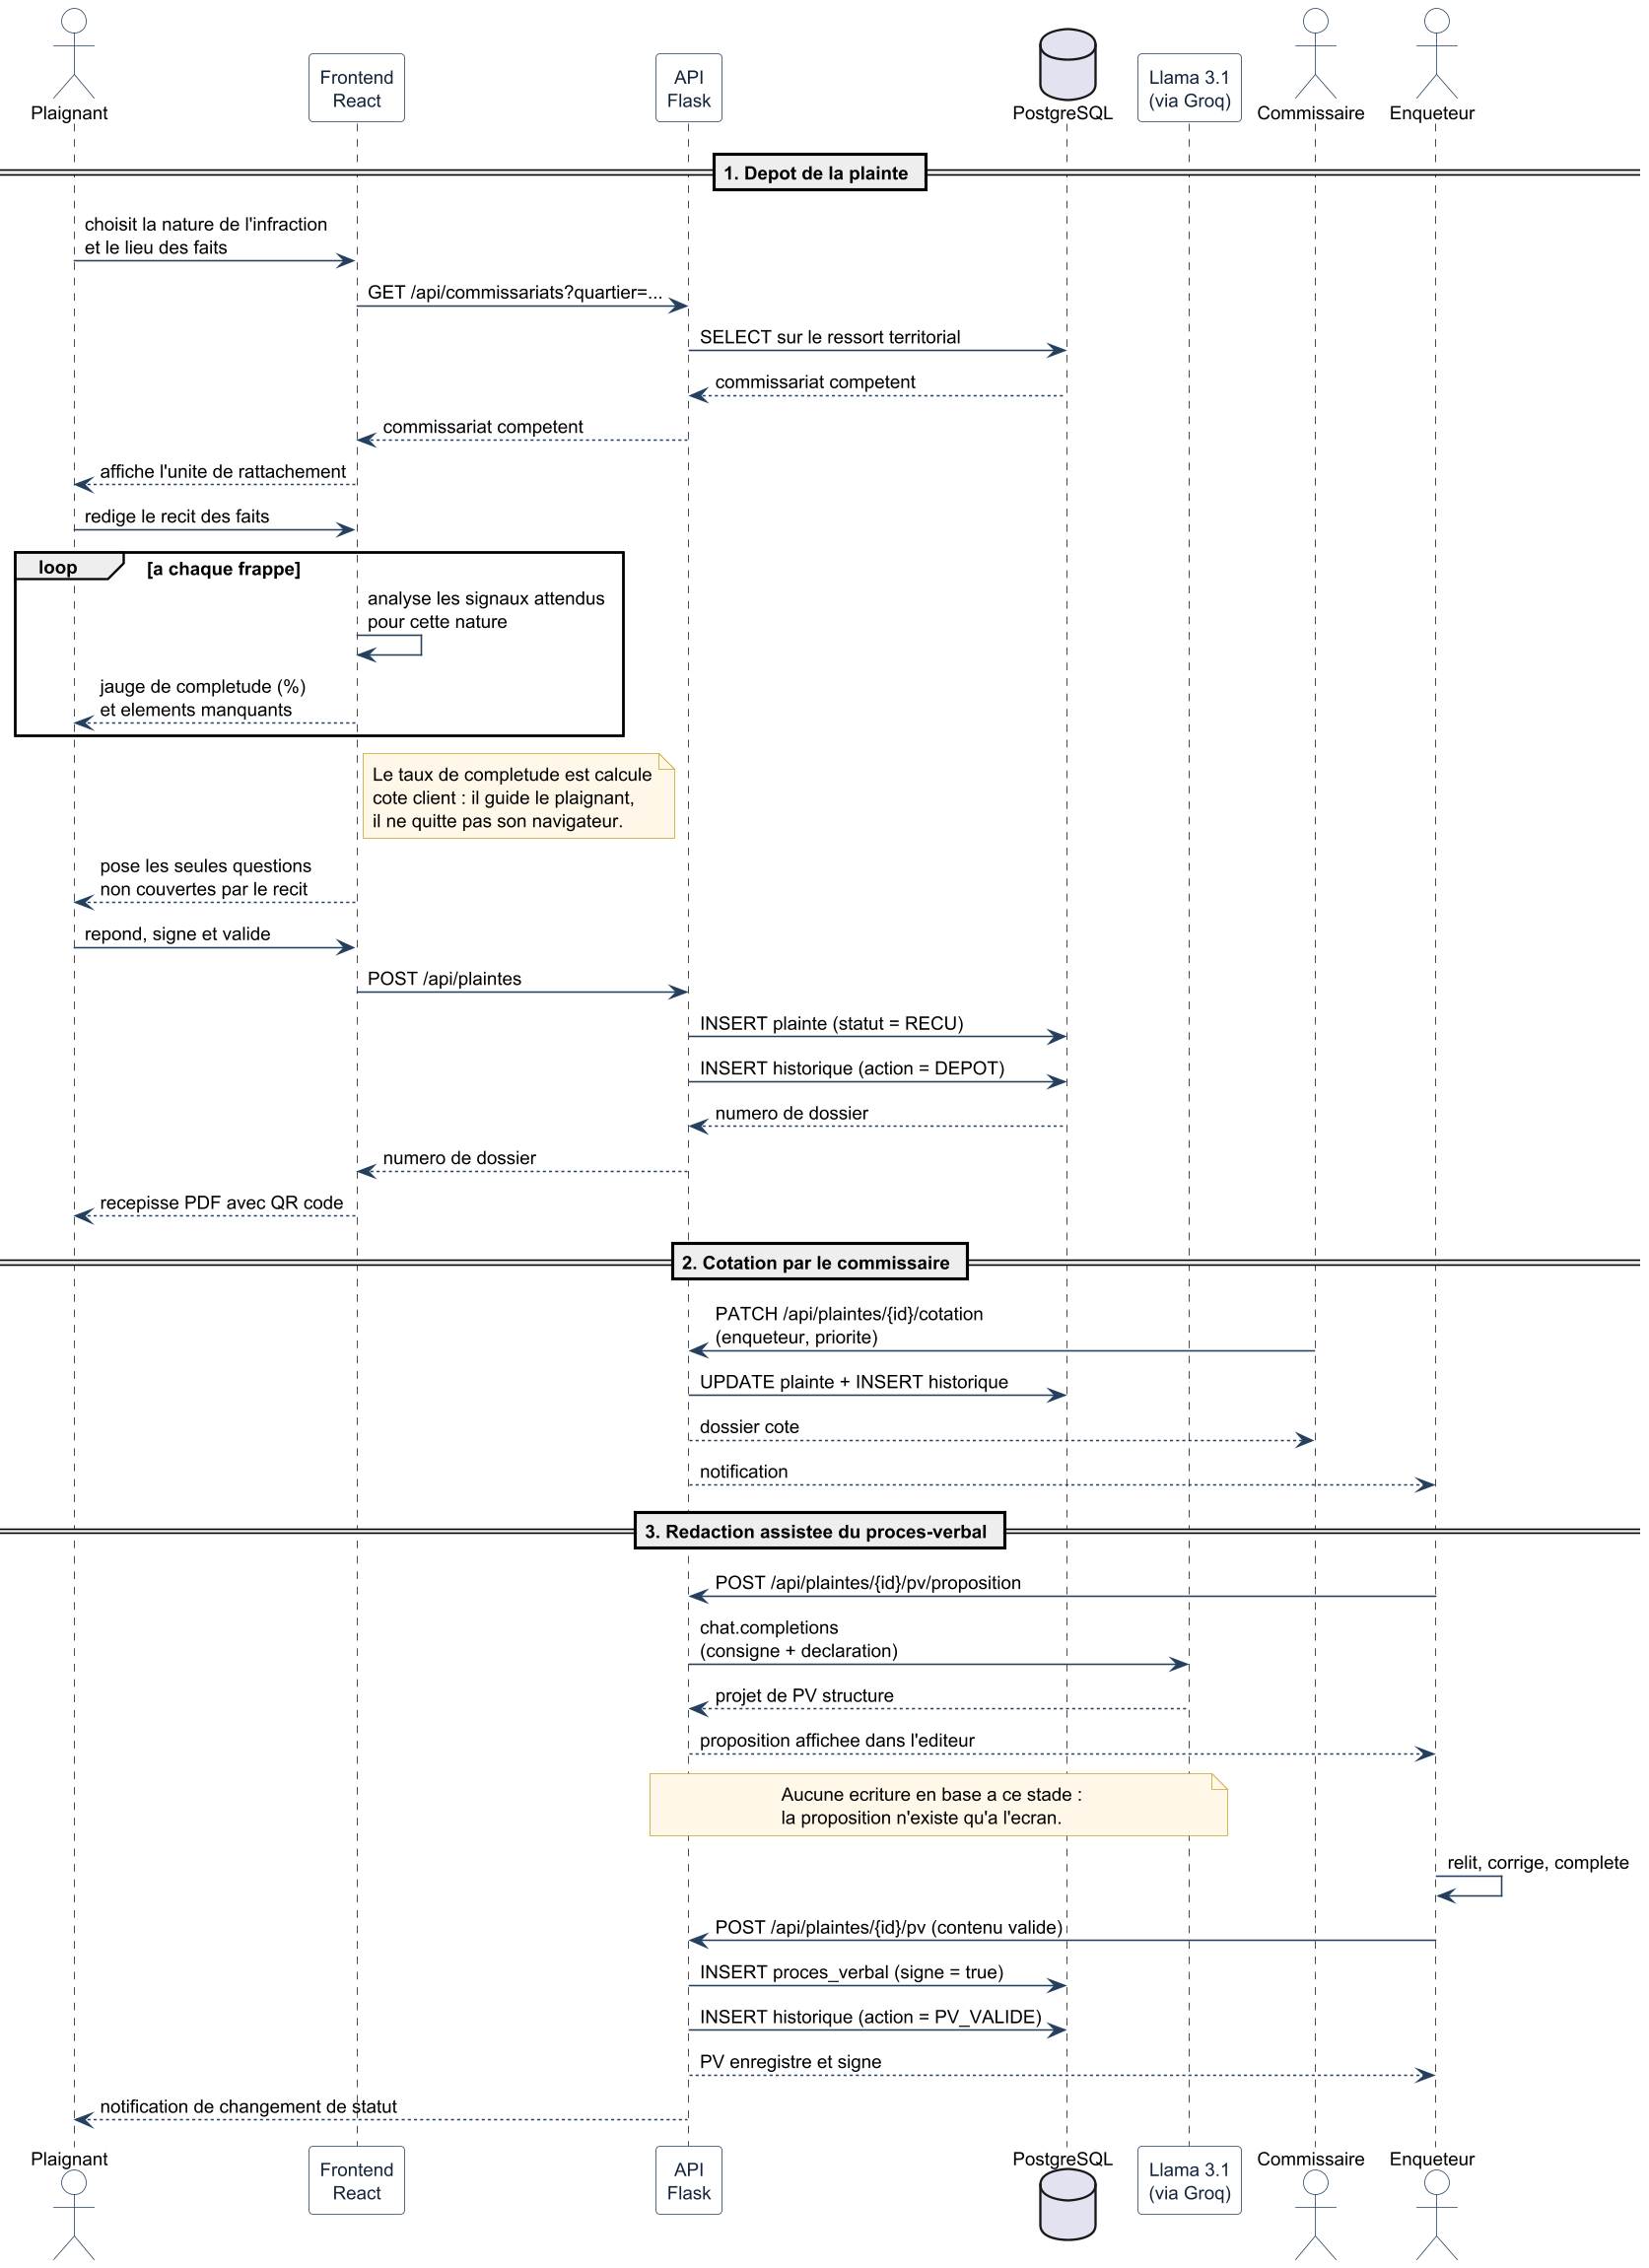
\includegraphics[width=\linewidth]{diagrammes/sequence.png}
    \caption{Diagramme de séquence : dépôt et instruction d'une plainte}
    \label{fig:sequence}
\end{figure}

La conception étant arrêtée, le chapitre suivant en présente la réalisation effective.
  % Chapitre 2
% CHAPITRE 3 — Réalisation de la plateforme PlainteCam

\chapter{Réalisation de la plateforme PlainteCam}
\label{ch:realisation}
\label{ch:bilan}

Le chapitre précédent a fixé ce que la plateforme doit faire et comment elle s'organise. Celui-ci rend compte de sa réalisation effective, puis de ce qu'elle vaut une fois construite.

Il s'ouvre sur le choix des outils et des technologies retenus pour porter la conception, puis sur l'architecture d'implémentation, qui montre comment ces technologies s'assemblent et communiquent. Il détaille ensuite la mise en œuvre de la solution, du parcours de dépôt jusqu'aux tests de recette. Il analyse alors les résultats obtenus en précisant la portée exacte des mesures, expose les apports pour l'organisation, formule les préconisations de pérennisation et dresse le bilan critique de la mission. Il se referme sur la présentation des interfaces effectivement livrées, qui donne à voir l'application réalisée.

\section{Choix des outils et technologies}

Réaliser la conception arrêtée au chapitre~\ref{ch:conception} supposait d'abord de choisir les technologies qui la porteraient. Ce choix a été guidé par trois contraintes issues du diagnostic : un public non technicien, une intégration d'intelligence artificielle sans friction, et un coût d'exploitation compatible avec les moyens d'une administration.

\subsection{Frontend : React.js}

Pour le frontend, React.js a été sélectionné après évaluation comparative des technologies d'interface utilisateur web les plus répandues. Vue.js offre une courbe d'apprentissage plus douce mais un écosystème plus restreint, tandis qu'Angular impose une structure complète dont la rigidité ne se justifiait pas à l'échelle du projet.

React a été retenu parce que ses composants permettent aux quatre espaces de partager les mêmes briques d'interface sans duplication, et parce que sa gestion d'état convient au formulaire de dépôt en cinq étapes, dont la saisie doit survivre à la navigation entre écrans.

\begin{figure}[H]
    \centering
    
\includegraphics[width=0.22\textwidth]{images/react.png}
    \caption{React.js, bibliothèque frontend}
    \label{fig:react}
\end{figure}

\subsection{Backend : Flask}

\textbf{Flask} a été retenu pour l'exposition des API et l'orchestration de la logique métier côté serveur. Ce micro-framework Python suit la spécification \textbf{WSGI} et laisse au développeur le choix de ses composants plutôt que d'imposer une pile complète, à la différence de Django dont les conventions nombreuses auraient alourdi un périmètre maîtrisé.

Flask a été retenu d'abord pour la \textbf{continuité de langage avec l'intelligence artificielle} : le client Python de Groq s'intègre au backend sans passerelle ni service intermédiaire, et c'est le critère qui a tranché. Il l'a été ensuite parce qu'un périmètre fonctionnel maîtrisé permet de choisir explicitement chaque brique plutôt que d'en hériter d'une pile imposée, avec SQLAlchemy pour la persistance et Flask-JWT-Extended pour l'authentification, pour une empreinte et un coût d'exploitation réduits derrière un serveur WSGI de production.

% La figure s'affiche automatiquement dès que images/flask.png existe.
\IfFileExists{images/flask.png}{%
\begin{figure}[H]
    \centering
    
\includegraphics[width=0.28\textwidth]{images/flask.png}
    \caption{Flask, micro-framework backend Python}
    \label{fig:flask}
\end{figure}
}{}

\subsection{Persistance : PostgreSQL et Supabase Storage}

Le \textbf{SGBD PostgreSQL} assure la persistance des données structurées. Son typage fort, ses types énumérés natifs pour les statuts, les priorités et les natures d'infraction, ainsi que son moteur transactionnel garantissent la cohérence des dossiers tout au long de l'enquête.

Les \textbf{pièces jointes} sont en revanche confiées à \textbf{Supabase Storage}, la base ne conservant que leurs métadonnées et le chemin de l'objet. Le dépôt est un \textbf{bucket privé} réservé aux utilisateurs authentifiés : aucune pièce n'est accessible par une URL publique, ce qui serait inacceptable pour un certificat médical ou l'identité d'un mis en cause. Ce choix répond directement au besoin de confidentialité (BNF1).

\subsection{Intelligence artificielle : Llama 3.1 servi par Groq}

La rédaction assistée des procès-verbaux s'appuie sur le modèle \textbf{Llama 3.1} de Meta, exploité via la plateforme d'inférence \textbf{Groq}, à ne pas confondre avec \textit{Grok}, le modèle de la société xAI. Son \textbf{palier gratuit} couvre les besoins du projet, son inférence rapide rend la proposition quasi instantanée, les poids ouverts de Llama autorisent un réhébergement ultérieur sur infrastructure maîtrisée, et l'appel reste exclusivement côté serveur : la clé d'API n'est jamais exposée au navigateur.

Le procès-verbal produit reste une \textbf{proposition}. Il est présenté à l'enquêteur dans un éditeur, qui le corrige et le valide avant signature. L'intelligence artificielle assiste la rédaction, elle ne se substitue pas à l'officier de police judiciaire, seul habilité à dresser le procès-verbal au sens du Code de procédure pénale~\cite{cameroun-cpp}. C'est la traduction technique du besoin de valeur probante (BNF3).

\begin{figure}[H]
    \centering
    
\includegraphics[width=0.34\textwidth]{images/grok_ai.png}
    \caption{Intelligence artificielle générative intégrée à PlainteCam}
    \label{fig:ia}
\end{figure}

\subsection{Environnement de développement}

Le développement s'est effectué sous \textbf{Windows 10}, avec \textbf{Visual Studio Code} pour l'édition du frontend React et du backend Python. Le versionnement est assuré par \textbf{Git} et \textbf{GitHub}. \textbf{Docker} conteneurise l'API et le SGBD : le backend Python et PostgreSQL s'exécutent ainsi dans un environnement Linux identique à celui visé en production, ce qui neutralise les écarts entre le poste de développement Windows et le serveur cible, qu'il s'agisse des chemins de fichiers, des fins de ligne ou des dépendances système. Enfin, \textbf{Postman} a servi à la recette des endpoints REST avant leur intégration au frontend.

\section{Architecture d'implémentation}

Ces technologies étant arrêtées, il reste à montrer comment elles s'assemblent et par quels protocoles elles communiquent.

La figure~\ref{fig:archi_implementation} traduit la conception en technologies. La plateforme suit une architecture \textbf{trois-tiers découplée} : le frontend React.js communique exclusivement avec le backend Flask via des API REST sécurisées par jeton. Le backend orchestre la logique métier, la persistance des données et les appels au service d'intelligence artificielle générative.

\begin{figure}[H]
    \centering
    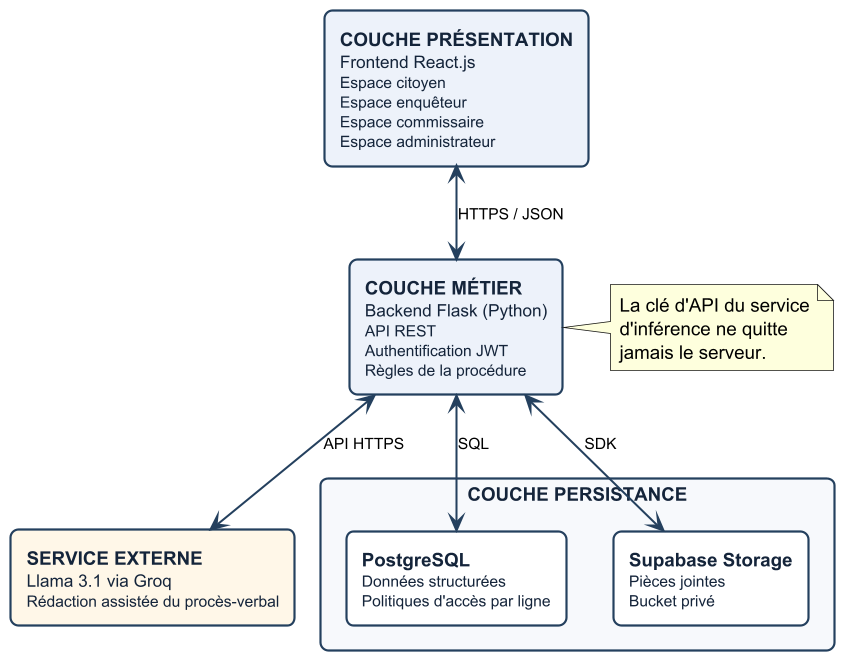
\includegraphics[width=0.78\textwidth]{diagrammes/architecture.png}
    \caption{Architecture d'implémentation : technologies et communications}
    \label{fig:archi_implementation}
\end{figure}

Les échanges portent chacun leur protocole : \textbf{HTTPS} et \textbf{JSON} entre la présentation et le métier, \textbf{SQL} vers PostgreSQL, un \textbf{SDK} vers le dépôt d'objets, et un appel \textbf{HTTPS} vers le service d'inférence. Cette dernière liaison n'existe qu'entre le backend et Groq, jamais depuis le navigateur. C'est ce qui garantit que la clé d'API ne quitte pas le serveur.

\section{Mise en œuvre de la solution}

Cette section décrit comment les besoins fonctionnels et non fonctionnels énoncés au chapitre précédent ont été effectivement implémentés, en partant du parcours le plus visible pour l'utilisateur pour aller vers les mécanismes qui le soutiennent.

\subsection{Parcours de dépôt du plaignant}

Le dépôt de plainte est implémenté comme un \textbf{formulaire séquentiel} en cinq écrans enchaînés :

\begin{enumerate}
    \item \textbf{Nature de l'infraction.} Choix parmi les natures gérées : vol simple, vol avec violence, agression physique, escroquerie, harcèlement, dégradation de biens, accident de la route, autre. Le \textbf{cumul est possible}, une même affaire pouvant relever de plusieurs qualifications, par exemple une escroquerie doublée d'un abus de confiance. Suit la cascade géographique Région, Département, Arrondissement, Quartier, dont le \textbf{commissariat compétent} est déduit automatiquement.
    \item \textbf{Déclaration des faits.} Récit libre du plaignant, avec dictée vocale optionnelle s'appuyant sur la Web Speech API du navigateur.
    \item \textbf{Identité du mis en cause.} Renseignée lorsqu'elle est connue, facultative dans le cas contraire.
    \item \textbf{Questions complémentaires.} Un jeu de questions propre à la nature de l'infraction est proposé. Celles dont la réponse figure déjà dans le récit des faits sont automatiquement écartées, afin de ne pas faire répéter le plaignant.
    \item \textbf{Aperçu et confirmation.} Récapitulatif de la déclaration, signature puis dépôt définitif, avec délivrance d'un \textbf{récépissé} portant le numéro de dossier.
\end{enumerate}

\paragraph{Analyse en direct de la déclaration.} Pendant que le plaignant rédige son récit, un bloc d'analyse affiche en continu un \textbf{taux de complétude} : la part des éléments attendus pour la nature d'infraction déclarée, à savoir l'objet concerné, le moment des faits, la description du suspect, les témoins et le justificatif, effectivement repérés dans le texte. Chaque élément apparaît sous forme d'étiquette, verte s'il est présent, rouge s'il manque, et une jauge situe le niveau atteint : rouge en dessous de 50~\%, orange de 50 à 80~\%, vert au-delà.

Ce pourcentage n'a qu'une seule fonction : \textbf{montrer au plaignant ce qui manque encore à sa déclaration}, afin qu'il le complète de lui-même avant de poursuivre. Il ne mesure ni la gravité des faits, ni l'avancement du dossier. Les éléments restés non détectés deviennent précisément les questions posées à l'étape 4, ce qui évite d'interroger le plaignant sur ce qu'il a déjà écrit.

\paragraph{Choix retenu pour la compétence territoriale.} L'audit a établi que le commissariat compétent peut être celui du lieu des faits \textbf{ou} celui du secteur de résidence du mis en cause. La plateforme retient le \textbf{lieu des faits}, seul critère systématiquement connu du plaignant au moment du dépôt, l'identité du mis en cause et a fortiori son adresse étant fréquemment ignorées. Ce choix ne ferme aucune option : le commissariat destinataire conserve la faculté de se dessaisir au profit d'une autre unité, le transfert étant alors inscrit au journal d'audit.

\subsection{Du dépôt à la clôture : le cycle de vie du dossier}

Une fois la plainte déposée, le dossier est rattaché au commissariat compétent et apparaît dans le tableau de bord du \textbf{commissaire}. Celui-ci procède à la \textbf{cotation} : il désigne l'\textbf{enquêteur} chargé de l'affaire et fixe la priorité du dossier.

L'enquêteur conduit ensuite l'instruction. Il convoque le plaignant et le mis en cause, tient les \textbf{auditions} et dresse les \textbf{procès-verbaux} correspondants. Chaque changement d'état est inscrit au journal d'audit. Le statut du dossier suit un cycle contraint par un type énuméré : \textit{Reçu}, \textit{Audition}, \textit{En instruction}, \textit{Décision}, \textit{Transmis}, \textit{Clôturé}. Le plaignant suit cette progression depuis son espace, sans avoir à se déplacer ni à téléphoner.

L'\textbf{avancement du dossier} est calculé comme la part de la procédure réellement accomplie : les étapes franchies, plus la fraction des actes déjà réalisés au sein de l'étape en cours. Un dossier transmis au parquet ou clôturé est à 100~\%. Cette valeur ne se saisit jamais à la main, de sorte qu'un dossier ne peut pas être déclaré avancé sans que les actes correspondants figurent effectivement au dossier. L'enquêteur la retrouve détaillée dans son \textbf{étapier}, une frise qui énumère pour chaque étape les actes requis et barre ceux qui sont accomplis ; le commissaire en suit la moyenne sur son tableau de bord.

Ces deux pourcentages ne mesurent donc pas la même chose et ne s'adressent pas aux mêmes personnes. La \textbf{complétude} qualifie la \textit{déclaration} et regarde le citoyen pendant qu'il rédige ; l'\textbf{avancement} qualifie la \textit{procédure} et regarde le commissaire qui supervise. Les confondre conduirait à présenter comme avancé un dossier simplement bien raconté, alors que rien n'y aurait encore été fait.

\subsection{Modèle de données}

Le schéma relationnel compte huit entités, dont le rôle est décrit ci-dessous.

\begin{itemize}
    \item \textbf{Commissariat.} Référentiel des commissariats et de leur ressort territorial, en lecture publique puisqu'il sert la cascade géographique du dépôt.
    \item \textbf{Profil.} Citoyens et personnels, porteurs du rôle applicatif qui détermine leurs droits.
    \item \textbf{Plainte.} Dossiers déposés et leur cycle de vie complet. Une plainte porte une ou plusieurs qualifications et un ou plusieurs préjudices, et n'est accessible qu'au plaignant et au commissariat saisi.
    \item \textbf{Pièce jointe.} Métadonnées des documents et photos, le fichier lui-même résidant dans le dépôt d'objets. L'accès est restreint au dossier de rattachement.
    \item \textbf{Procès-verbal.} Procès-verbaux d'audition proposés par l'intelligence artificielle puis validés par l'enquêteur, accessibles à ce dernier seul.
    \item \textbf{Convocation.} Convocations émises et suites données, visibles du commissariat émetteur.
    \item \textbf{Historique.} Journal d'audit de toutes les transitions de statut, en lecture seule y compris pour les administrateurs.
    \item \textbf{Notification.} Messages adressés au plaignant et aux personnels, visibles de leur seul destinataire.
\end{itemize}

\subsection{Sécurité et contrôle d'accès}

L'authentification repose sur des jetons \textbf{JWT}~\cite{jwt-rfc} signés côté serveur. Le citoyen s'identifie par adresse électronique et code à usage unique ; les personnels par matricule et mot de passe. Chaque requête est ensuite autorisée selon le rôle porté par le jeton : un plaignant n'accède qu'à ses propres dossiers, un enquêteur à ceux qui lui ont été cotés, un commissaire à l'ensemble des dossiers de son commissariat. Ce cloisonnement est doublé au niveau du SGBD par des politiques d'accès par ligne, de sorte qu'une requête mal formée ne puisse pas contourner la règle métier. C'est ce double verrou, applicatif et base de données, qui satisfait le besoin de confidentialité (BNF1).

\subsection{Tests effectués}

La recette a été conduite manuellement sur un jeu de dossiers de test couvrant les huit natures d'infraction gérées. Elle a porté sur quatre familles de scénarios, dont le détail figure en annexe~C.

Les \textbf{tests fonctionnels} ont vérifié le dépôt complet d'une plainte sur les cinq étapes du parcours, la détermination du commissariat compétent par cascade géographique, et la cotation d'un dossier à un enquêteur avec fixation de la priorité. Les trois se sont révélés conformes.

Le \textbf{test d'intelligence artificielle} a porté sur la rédaction d'un procès-verbal à partir de la déclaration du plaignant. Le résultat est conforme, sous la réserve constante que la relecture de l'enquêteur reste requise.

Les \textbf{tests de sécurité} ont cherché à mettre le cloisonnement en défaut. La consultation d'un dossier tiers par un citoyen non plaignant a été refusée, de même que l'appel d'un point d'accès sans jeton valide, rejeté par un code HTTP 401. Dans les deux cas, c'est le refus qui constitue le succès du test.

Les \textbf{tests documentaires et de qualité} ont contrôlé la génération des PDF du récépissé et du procès-verbal ainsi que la validité du QR code, tous conformes. La fidélité de la transcription vocale, en revanche, n'est que partiellement satisfaisante et impose une relecture.

Deux limites sont assumées à ce stade. La dictée vocale fonctionne sur l'ensemble des navigateurs testés, mais la \textbf{fidélité de la transcription reste imparfaite} : le texte obtenu ne restitue pas toujours exactement les propos du plaignant, en particulier sur les noms propres, les toponymes et les tournures propres au français parlé localement. Une relecture à l'écran est donc indispensable avant de passer à l'étape suivante, et la dictée est présentée comme une aide à la saisie plutôt que comme un mode de déclaration autonome. Par ailleurs, aucun test de charge n'a été mené faute d'environnement de production représentatif. Ces deux points figurent dans les préconisations formulées plus loin.

\section{Analyse des résultats}

La plateforme étant réalisée et testée, reste à établir ce qu'elle change effectivement, et avec quel degré de certitude.

\subsection{Méthode de mesure}

Les résultats présentés ci-dessous ont été relevés en \textbf{recette}, sur un jeu de dossiers de test couvrant les huit natures d'infraction gérées, et non en exploitation réelle. Les valeurs « avant » décrivent la procédure telle que l'audit l'a documentée ; les valeurs « après » ont été relevées sur la plateforme.

Une précision de méthode s'impose ici. Le mémoire \textbf{n'avance aucun chiffre sur la durée de cotation d'un dossier ni sur celle de traitement d'une affaire}. Ces durées relèvent de la connaissance interne du commissariat, varient fortement selon l'affluence, la nature des faits et la disponibilité des enquêteurs, et aucune source ne permettait de les établir : c'est précisément l'absence de traçabilité qui les rend inconnaissables. Les avancer aurait été une extrapolation. Le tableau ne compare donc que ce qui a pu être constaté de part et d'autre, et signale explicitement, en dernière ligne, ce que la plateforme rend désormais \textbf{mesurable} sans prétendre en connaître la valeur.

\begin{table}[H]
    \centering
    \begin{tabularx}{\textwidth}{|>{\raggedright\arraybackslash}X|>{\raggedright\arraybackslash}p{2.4cm}|>{\raggedright\arraybackslash}p{2.9cm}|>{\raggedright\arraybackslash}p{2.2cm}|}
        \hline
        \textbf{Indicateur} & \textbf{Avant} & \textbf{Après} & \textbf{Nature} \\
        \hline
        Déplacement pour déposer plainte & Obligatoire & Supprimé & Mesuré \\
        \hline
        Saisie de la déclaration par le plaignant & Au guichet, tributaire de l'affluence & $<$ 8 min en ligne & Mesuré \\
        \hline
        Détermination du commissariat compétent & Oralement au guichet & Automatique, par le lieu des faits & Mesuré \\
        \hline
        Mise en forme d'un procès-verbal & Manuscrite, sur template papier & Proposition structurée en $<$ 2 min, à réviser & Mesuré \\
        \hline
        Complétude de la déclaration & Variable selon l'aisance du plaignant & Questions ciblées et score de complétude & Mesuré \\
        \hline
        Traçabilité des actes de procédure & Registre papier & 100\% horodatée & Mesuré \\
        \hline
        Suivi du dossier par le plaignant & Déplacement nécessaire & Disponible en ligne & Mesuré \\
        \hline
        Remise de la convocation au mis en cause & À la charge du plaignant & Notification par la plateforme & Mesuré \\
        \hline
        Délai entre dépôt et cotation & \textbf{Non mesurable} & Horodaté, donc mesurable & Nouvelle capacité \\
        \hline
        Taux d'erreur dans les procès-verbaux & Non mesuré & Non mesuré & À instrumenter \\
        \hline
    \end{tabularx}
    \caption{Comparaison des indicateurs avant et après PlainteCam}
    \label{tab:resultats}
\end{table}

\subsection{Portée et limites des mesures}

Trois réserves doivent accompagner la lecture de ce tableau. D'abord, les durées « après » sont celles d'un utilisateur accompagné en recette, non celles d'un citoyen livré à lui-même ; l'écart réel sera plus élevé. Ensuite, la proposition de procès-verbal produite en moins de deux minutes doit encore être relue et corrigée par l'enquêteur : le gain porte sur la mise en forme et la structuration, non sur l'appréciation juridique des faits. Enfin, aucun test de charge n'a été mené, faute d'environnement de production représentatif ; les temps de réponse observés ne préjugent pas du comportement de la plateforme en usage réel.

Il faut ajouter que la plateforme n'agit pas sur ce que l'audit a identifié comme la principale source de contentieux : le refus, par le mis en cause, de signer un procès-verbal dont il conteste la fidélité. La plateforme en conserve la trace horodatée, mais la situation reste entière. Annoncer une réduction des délais de traitement serait donc doublement infondé, faute de mesure initiale, et parce que ce facteur de blocage échappe à l'outil.

\section{Apports pour l'organisation}

Les mesures qui précèdent se traduisent, pour le commissariat, par quatre gains de nature différente.

\textbf{Gain de temps :} La suppression du déplacement et le rattachement automatique au commissariat compétent retirent de la chaîne les étapes de circulation physique qui précédaient toute action d'enquête. La rédaction assistée libère par ailleurs l'enquêteur d'une part importante du travail de mise en forme. L'ampleur de ce gain reste à établir en exploitation : elle dépend de la charge du service, que seul le commissariat connaît.

\textbf{Gain de qualité :} Le questionnaire complémentaire garantit qu'aucune information déterminante pour la nature d'infraction déclarée n'est omise au dépôt, là où la retranscription orale dépendait de la disponibilité et de l'expérience de l'agent de permanence.

\textbf{Gain de visibilité :} Le commissaire dispose pour la première fois d'indicateurs consolidés, qu'il s'agisse des volumes, des répartitions ou de la charge par enquêteur, pour piloter l'activité de son unité.

\textbf{Gain de traçabilité :} Chaque acte étant horodaté et attribué, la reconstitution d'une procédure devient immédiate, ce qui sert autant l'audit interne que la réponse aux demandes de l'autorité judiciaire.

\section{Préconisations}

Pour pérenniser et faire évoluer PlainteCam après la fin du stage, les préconisations suivantes sont formulées :

\begin{itemize}
    \item \textbf{Instrumenter la plateforme avant le déploiement :} enregistrer les durées réelles de dépôt, de cotation et de clôture afin de disposer d'indicateurs mesurés en exploitation, et non plus estimés en recette. C'est la condition pour objectiver le gain auprès de la hiérarchie.
    \item \textbf{Conduire un test de charge} représentatif du volume d'un commissariat urbain avant la mise en service.
    \item \textbf{Former les personnels}, en insistant sur la révision des procès-verbaux proposés par l'intelligence artificielle : le risque principal est la validation sans relecture d'un texte plausible mais inexact.
    \item \textbf{Améliorer la fidélité de la transcription vocale}, aujourd'hui inégale sur les noms propres et les toponymes. Une transcription côté serveur, entraînée ou adaptée au français parlé au Cameroun, corrigerait ce défaut. Tant qu'il subsiste, la relecture du texte dicté doit rester obligatoire avant validation.
    \item \textbf{Vérifier les quotas du service d'inférence avant la mise en service :} le projet fonctionne sur le palier gratuit de Groq, dont les limites de requêtes conviennent à un pilote, mais pas nécessairement au volume d'un commissariat urbain. Deux issues sont possibles selon l'arbitrage budgétaire, souscrire une offre payante ou réhéberger Llama sur un serveur de l'institution, ce que ses poids ouverts autorisent.
    \item \textbf{Désigner un référent technique interne} chargé des mises à jour, de la correction des anomalies et de l'évolution de la plateforme.
    \item \textbf{Déployer progressivement}, en commençant par un commissariat pilote, avant extension au reste du ressort.
\end{itemize}

\section{Bilan critique de la mission}

Au-delà des résultats mesurés, la conduite du projet appelle un retour réflexif sur ce qui a facilité le travail et ce qui l'a entravé.

\subsection{Ce qui a fonctionné}

Quatre choix se sont révélés payants au fil de la mission.

\begin{itemize}
    \item La méthodologie Agile a permis de livrer des fonctionnalités utilisables dès le deuxième sprint, facilitant les retours précoces des parties prenantes.
    \item Le choix de Python pour le backend a supprimé toute friction dans l'intégration de l'intelligence artificielle générative, qui s'est faite plus vite que prévu.
    \item L'architecture découplée entre frontend et backend a permis un développement parallèle efficace des deux couches.
    \item Le questionnaire complémentaire, conçu avec les personnels du commissariat, s'est révélé mieux accepté que la génération automatique seule, parce qu'il laisse la main au plaignant.
\end{itemize}

\subsection{Ce qui a posé des défis}

Quatre difficultés ont en revanche pesé sur le déroulement du projet.

\begin{itemize}
    \item La modélisation géographique en cascade a demandé plus de temps que prévu, les données de référence des quartiers étant incomplètes et hétérogènes.
    \item La gestion des droits d'accès par rôle a nécessité plusieurs itérations avant d'atteindre un niveau de cloisonnement satisfaisant entre plaignant, enquêteur et commissaire.
    \item La question de la valeur probante du dossier numérique a été sous-estimée au départ : elle relève autant du juridique que de la technique et aurait mérité d'être instruite dès la conception.
    \item La conduite du changement auprès des personnels a demandé un effort de formation et de communication plus important que planifié.
\end{itemize}

\subsection{Enseignements tirés}

Cette mission a confirmé l'importance d'impliquer les utilisateurs finaux dès la phase de conception pour éviter les allers-retours coûteux en fin de projet. Elle a également montré qu'un projet de dématérialisation dans un contexte régalien ne se réduit pas à un problème technique : les dimensions juridiques et organisationnelles conditionnent l'adoption autant que la qualité du logiciel. Enfin, elle a mis en évidence la nécessité d'instrumenter une plateforme dès sa conception, faute de quoi la démonstration de sa valeur repose sur des estimations plutôt que sur des mesures.

\section{Résultats : interfaces de la plateforme}

Cette dernière section donne à voir le produit fini. Chaque interface y est rapportée au besoin fonctionnel qu'elle satisfait.

\subsection{Tableau de bord du commissaire}

\begin{figure}[H]
    \centering
    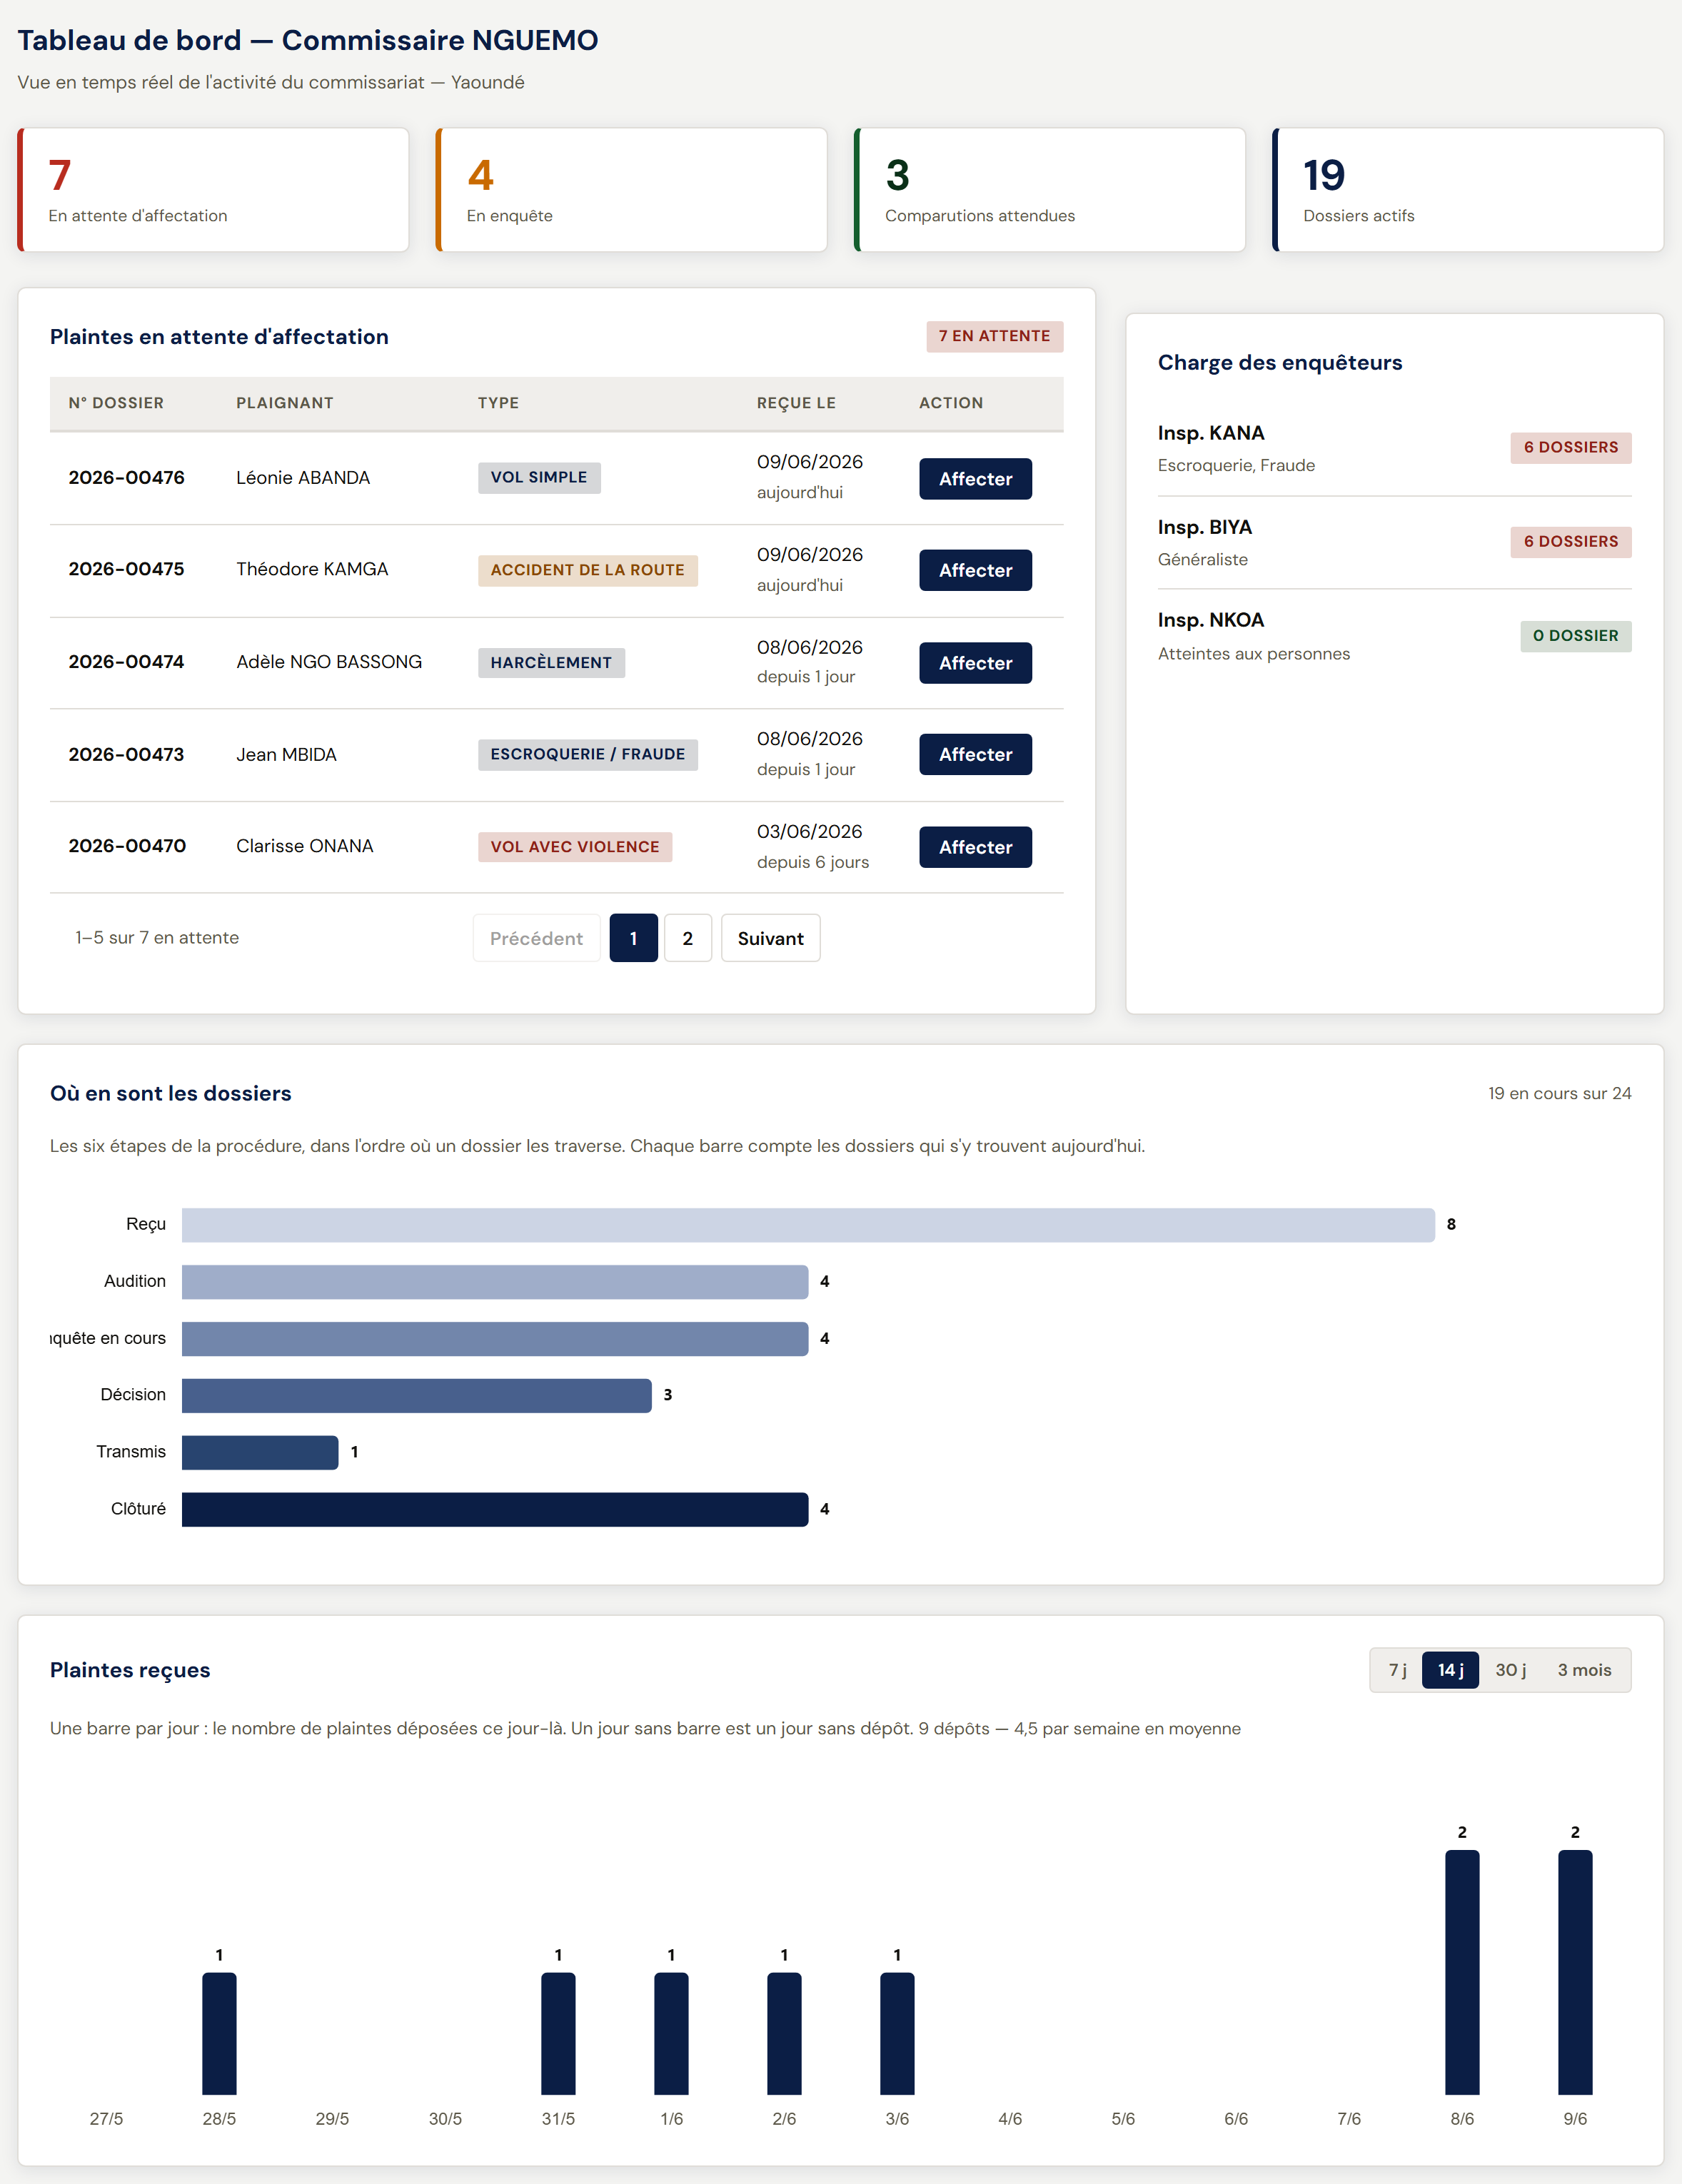
\includegraphics[width=0.58\textwidth]{images/dashboard.png}
    \caption{Tableau de bord du commissaire, vue générale}
    \label{fig:dashboard}
\end{figure}

Le tableau de bord réunit quatre indicateurs, à savoir les plaintes enregistrées, les dossiers achevés, le délai moyen de traitement et l'\textbf{avancement moyen des dossiers}, ainsi que la liste des dossiers récents et l'accès direct à la cotation. Le commissaire y trouve la vision d'ensemble de son unité que la procédure papier ne permettait pas sans dépouillement manuel du registre (BF8).

\subsection{Dépôt d'une plainte}

\begin{figure}[H]
    \centering
    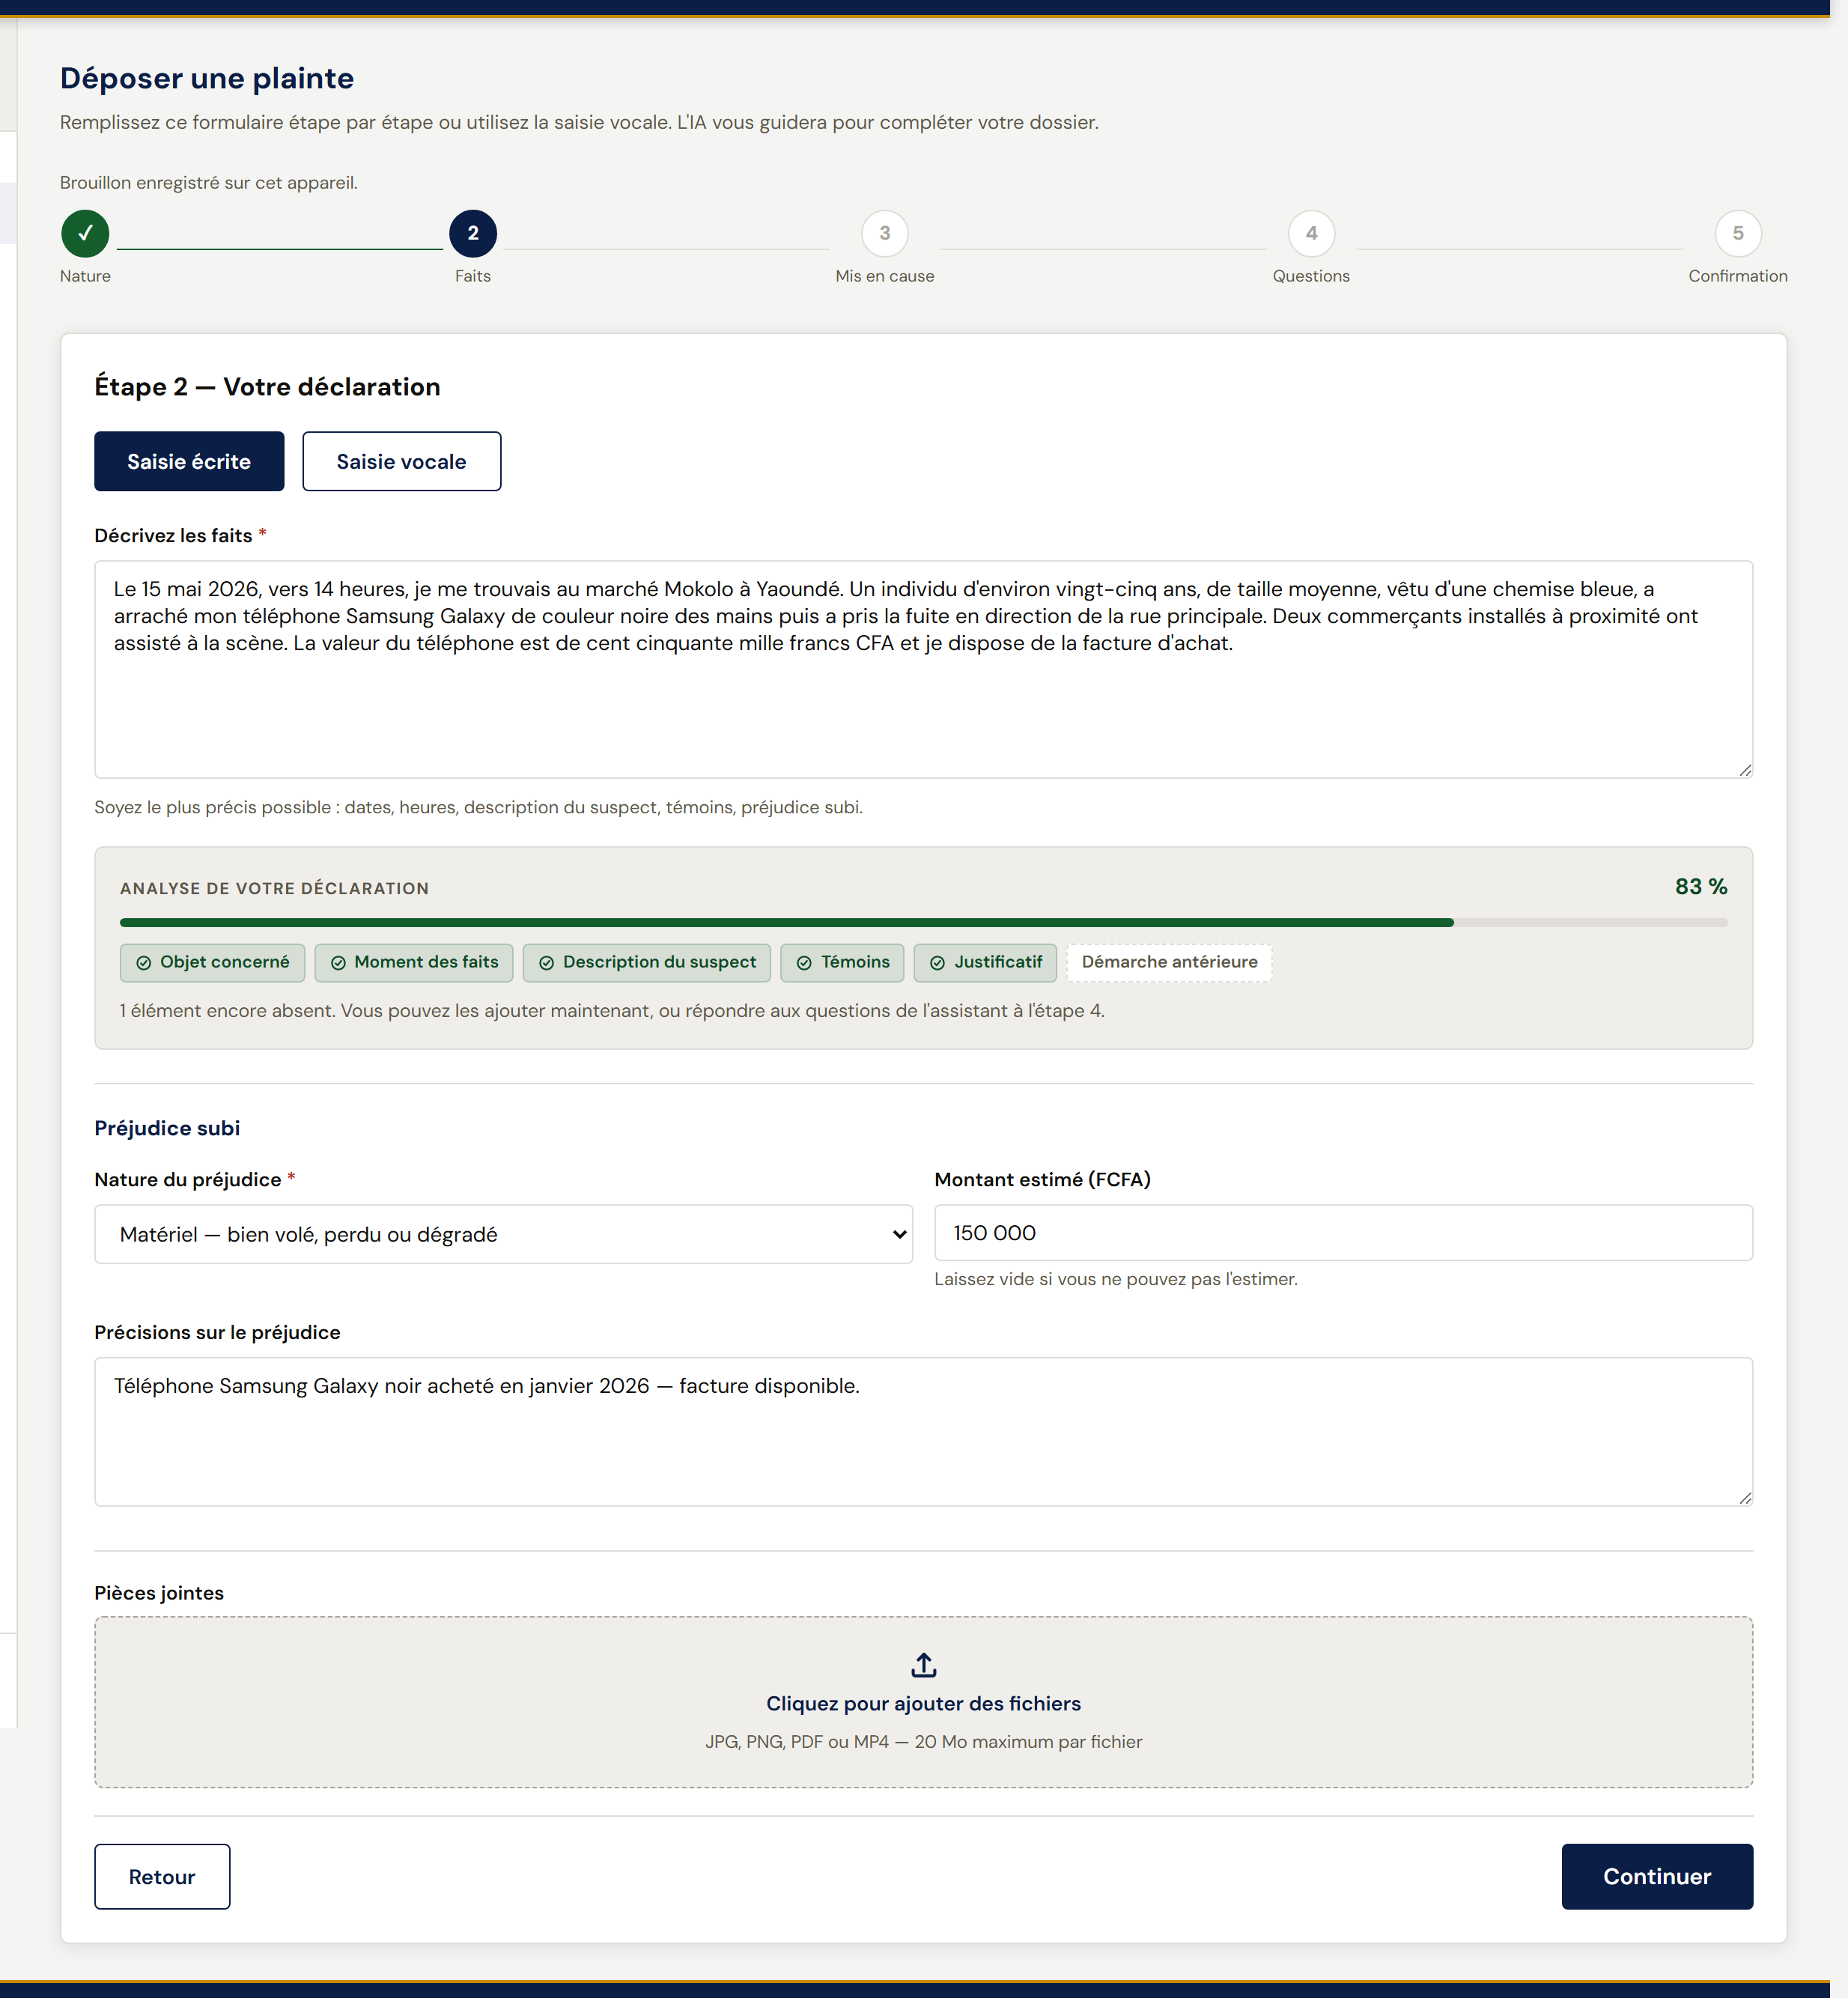
\includegraphics[width=0.58\textwidth]{images/modelisation.png}
    \caption{Parcours de dépôt guidé, formulaire en 5 étapes}
    \label{fig:soumission}
\end{figure}

Le parcours enchaîne le choix de la nature de l'infraction, la cascade géographique qui détermine le commissariat compétent, le récit libre des faits avec dictée vocale optionnelle, l'identité du mis en cause et les questions complémentaires. Une plainte peut ainsi être déposée intégralement en ligne, par un public non technicien et sans déplacement (BF1 et BF2).

\subsection{Instruction du dossier par l'enquêteur}

\begin{figure}[H]
    \centering
    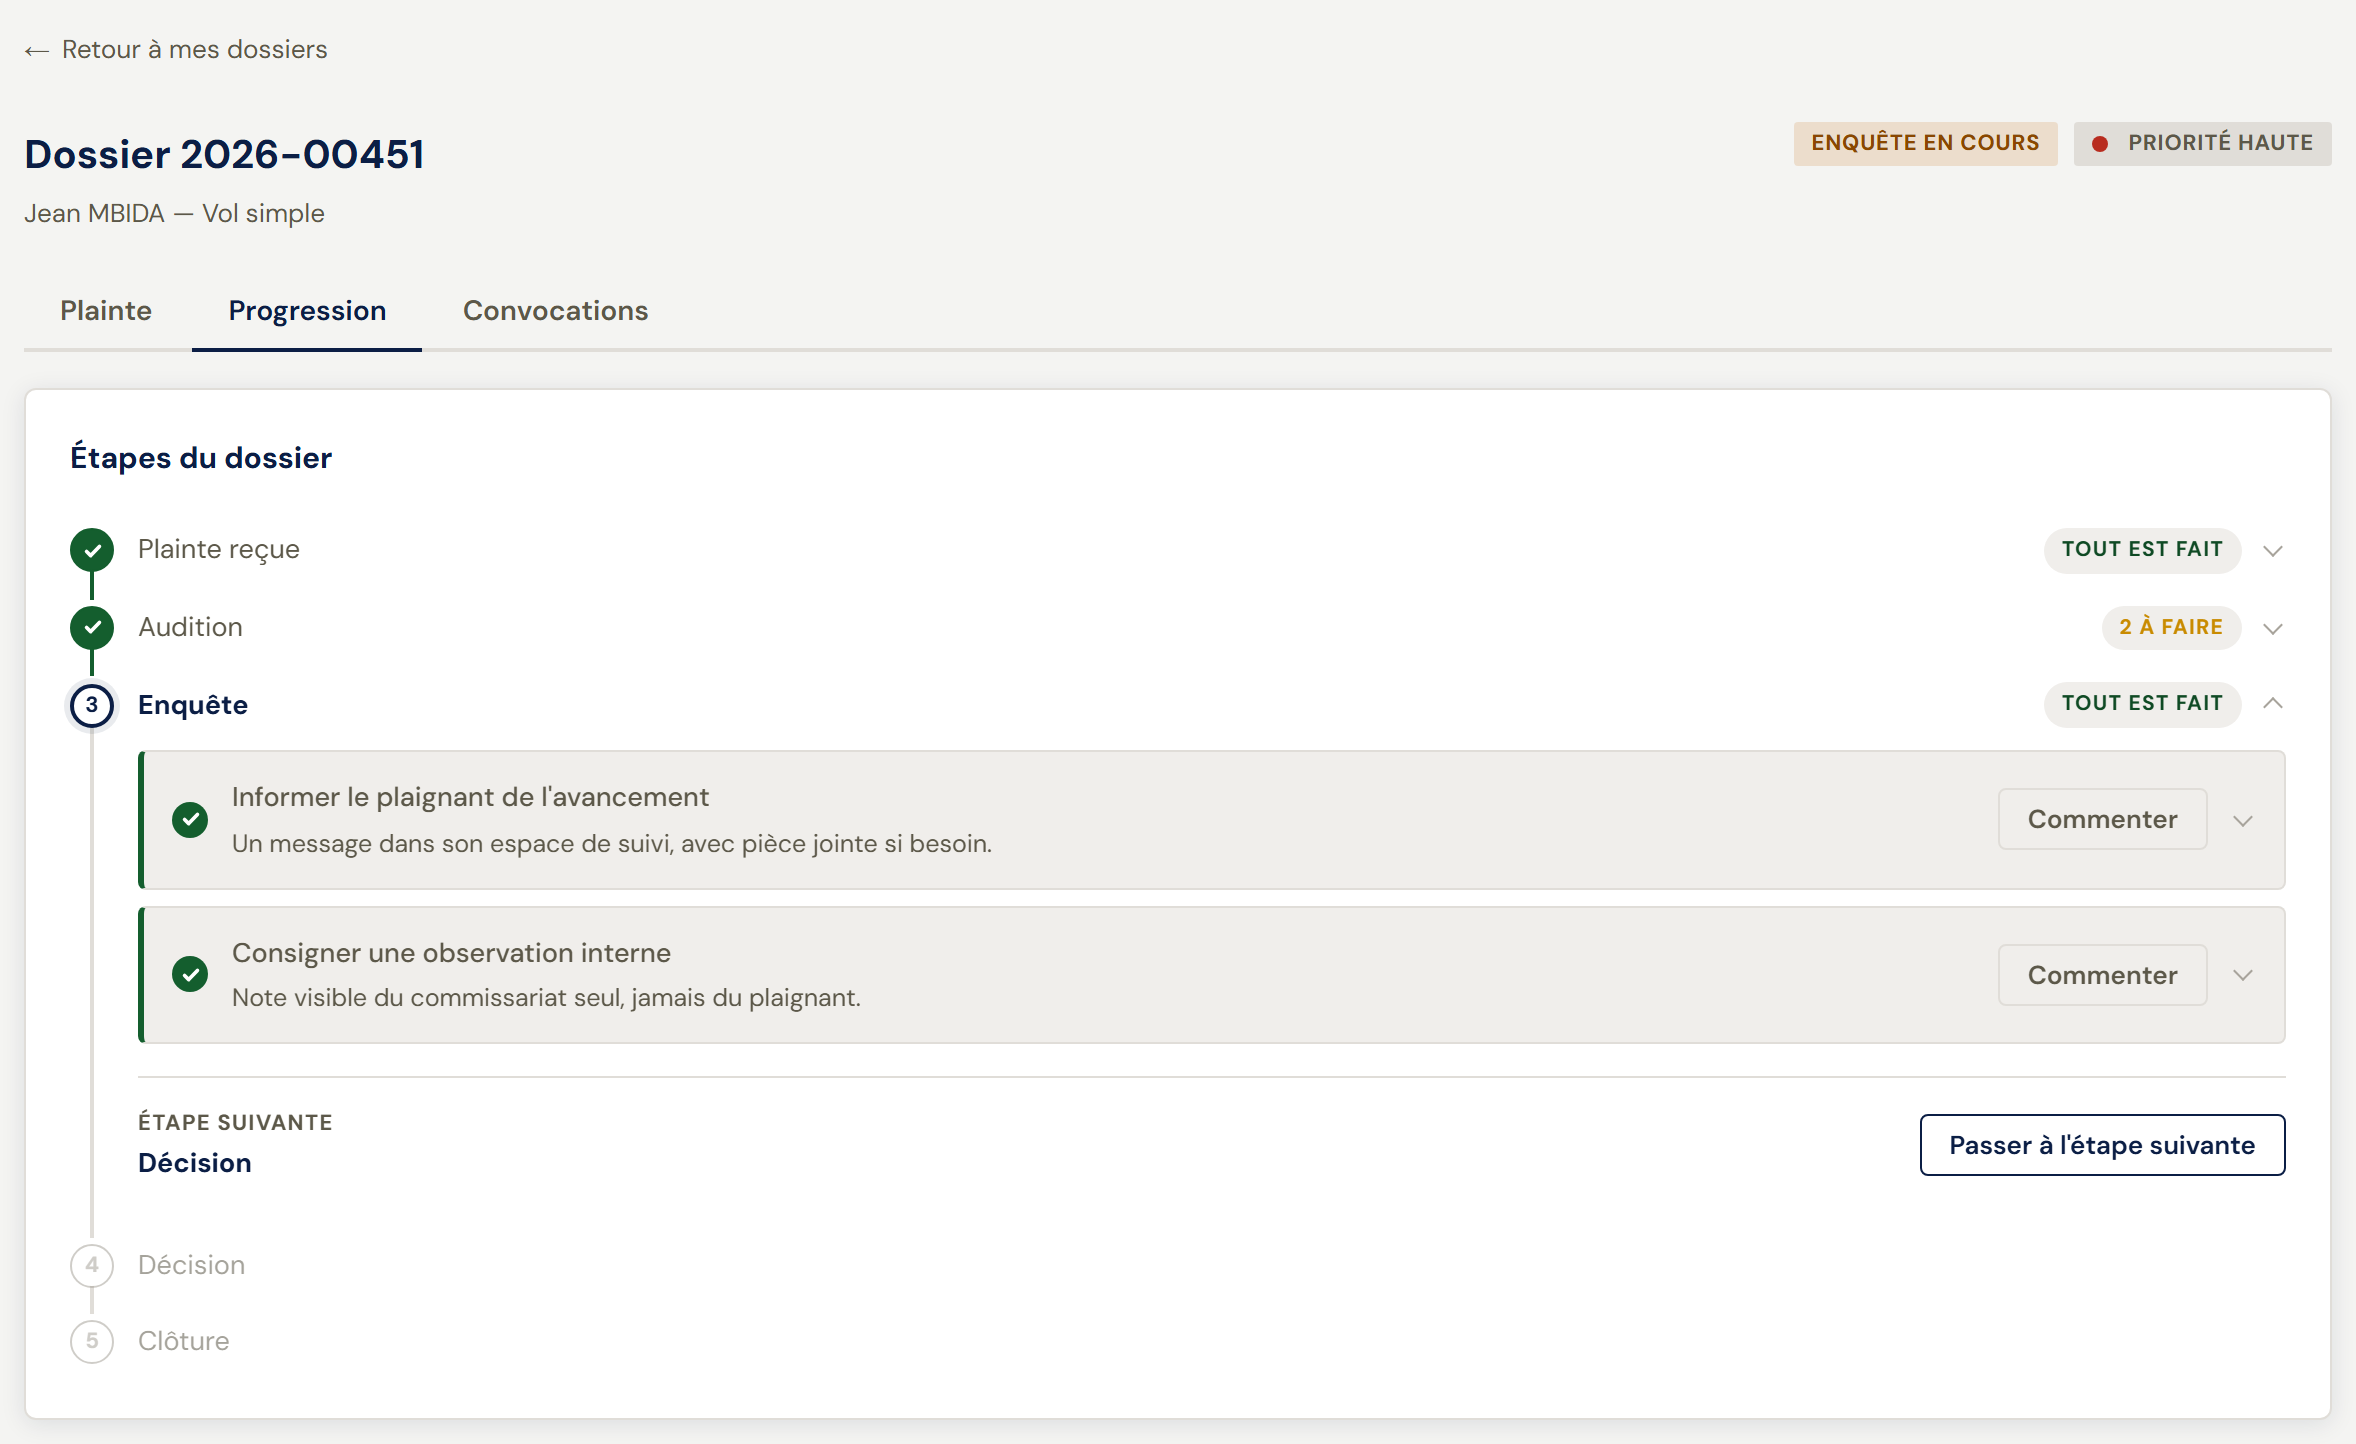
\includegraphics[width=0.58\textwidth]{images/configuration.png}
    \caption{Espace enquêteur, instruction d'un dossier et procès-verbal}
    \label{fig:configuration}
\end{figure}

L'enquêteur consulte le dossier coté, révise dans un éditeur le procès-verbal d'audition pré-rédigé, le valide, le signe et émet la convocation. Il part d'un document déjà structuré à partir de la déclaration du plaignant plutôt que d'une page blanche, sans que sa responsabilité en soit entamée : aucun procès-verbal n'est enregistré sans sa validation explicite (BF5).

\subsection{Gestion des dossiers cotés}

\begin{figure}[H]
    \centering
    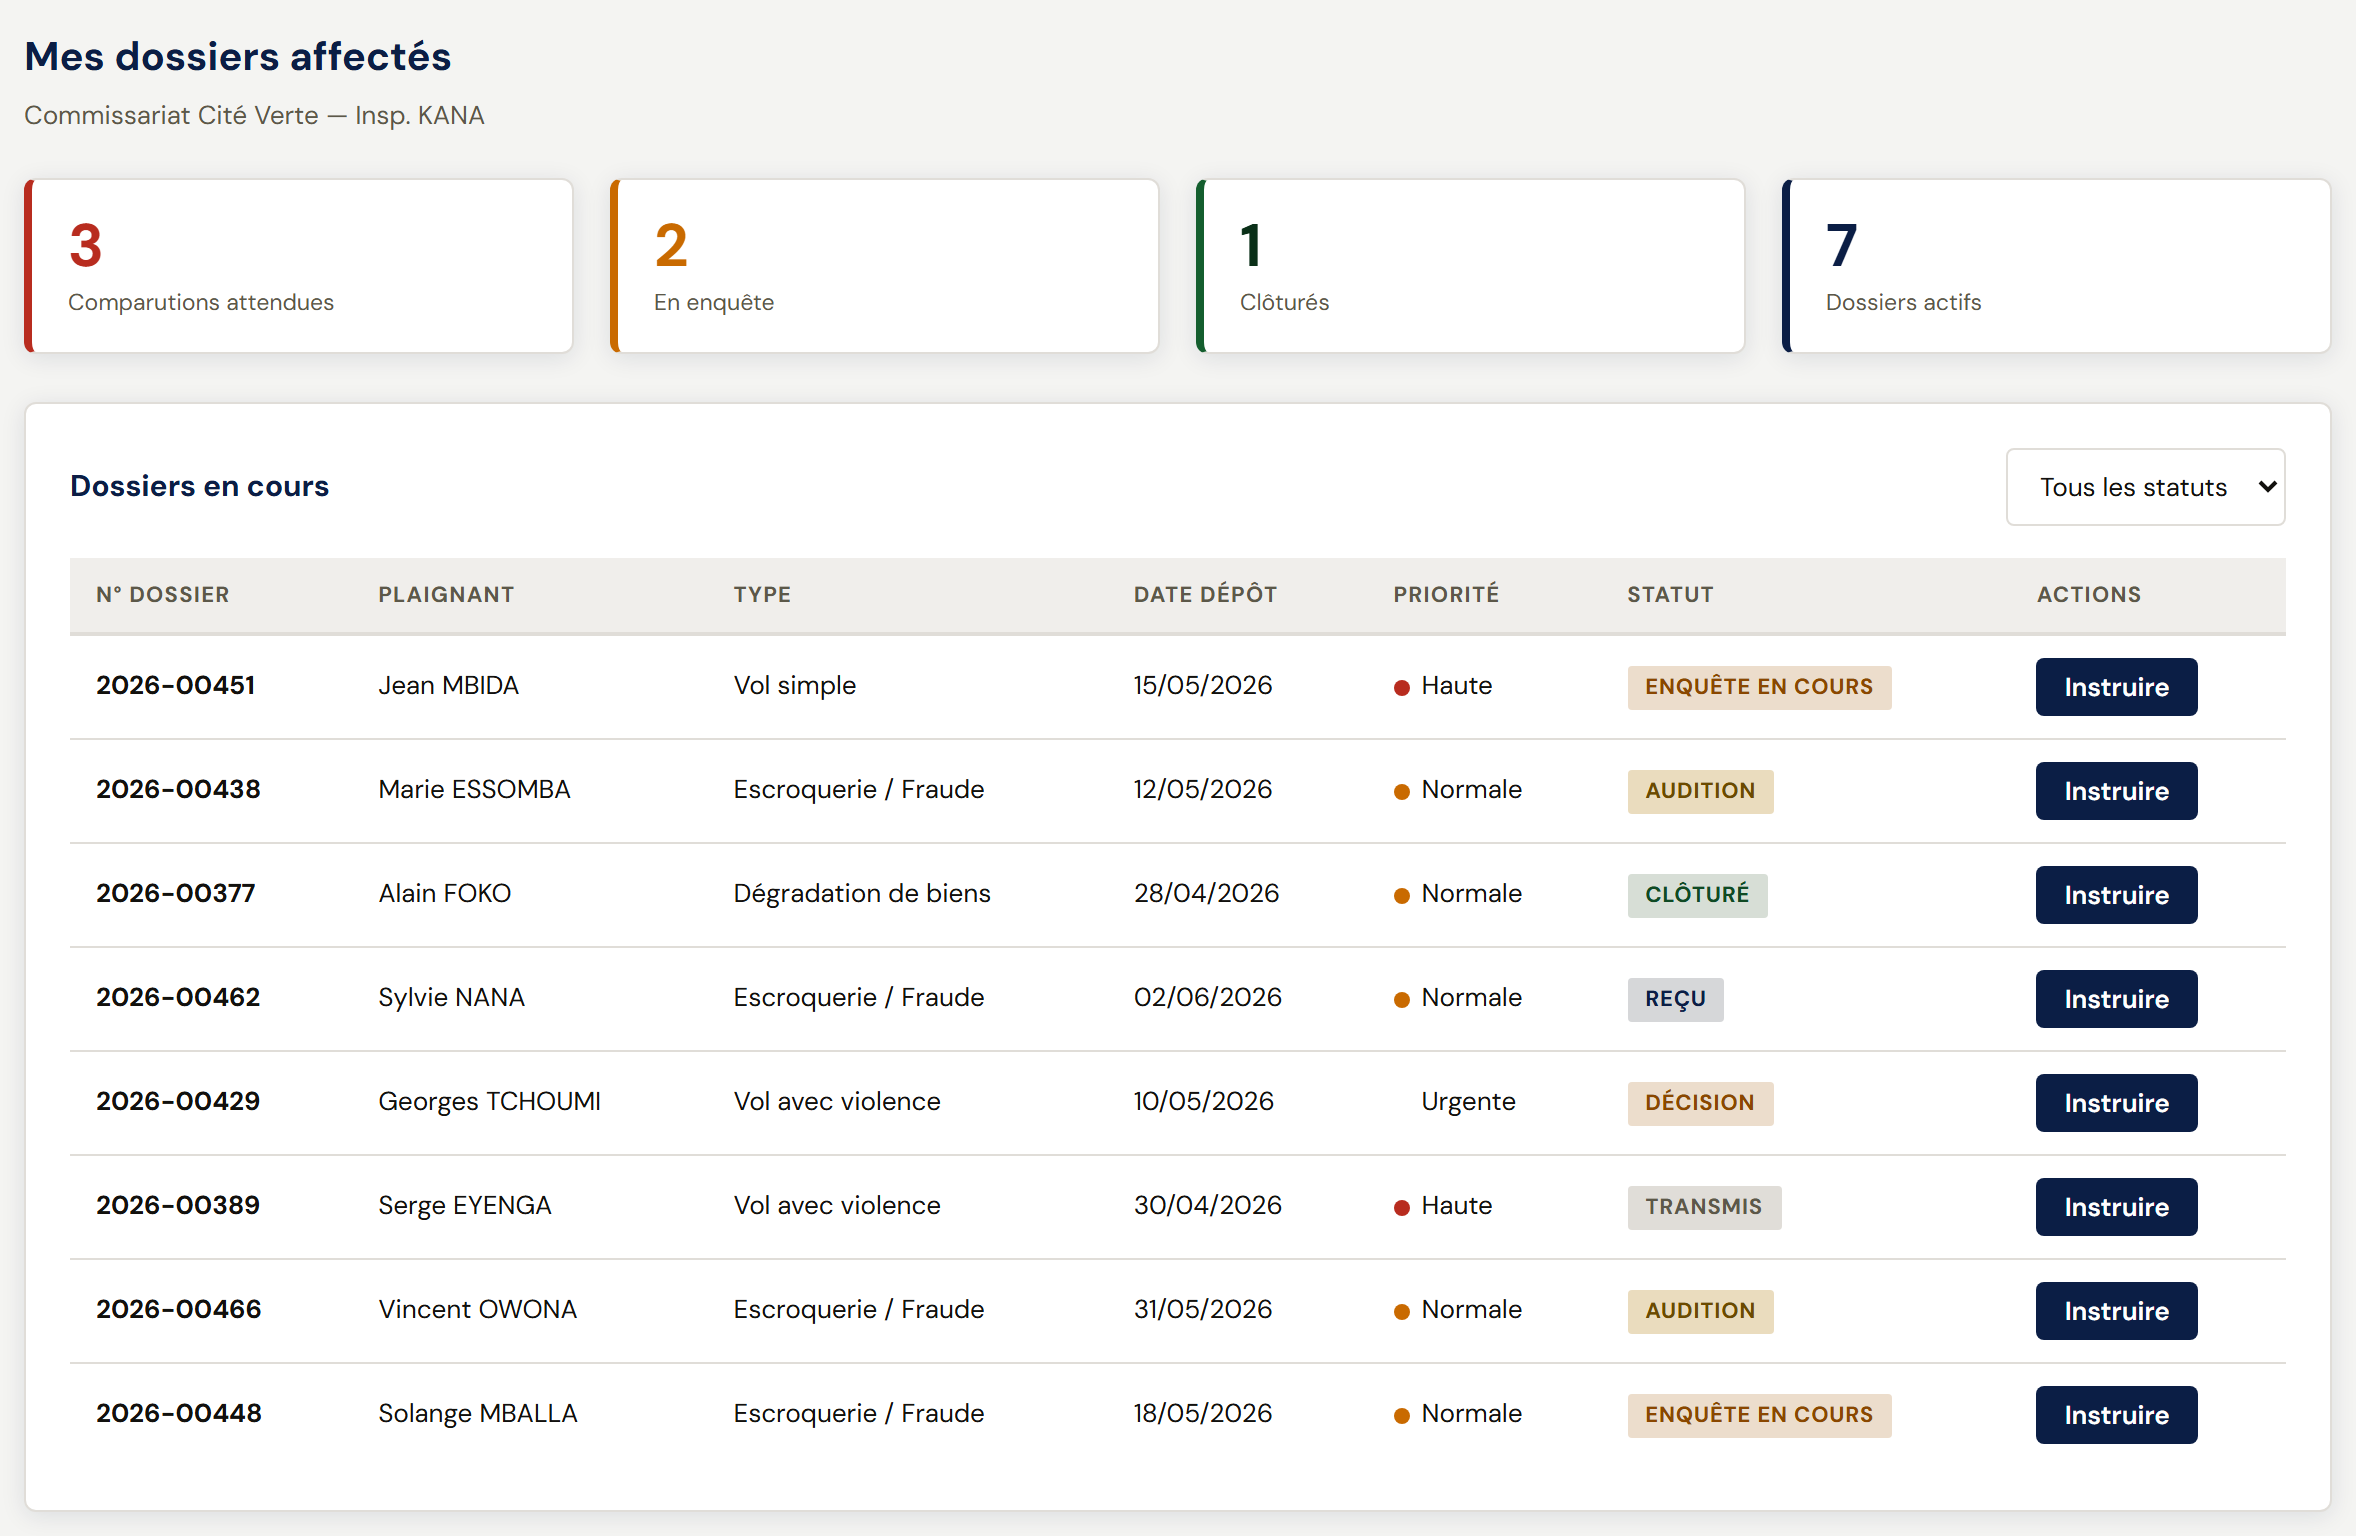
\includegraphics[width=0.58\textwidth]{images/task.png}
    \caption{Liste des dossiers cotés à l'enquêteur}
    \label{fig:taches}
\end{figure}

Chaque enquêteur dispose de son portefeuille de dossiers, classés par statut, filtrables par priorité et assortis d'actions rapides. Cette information était auparavant dispersée entre le registre et les chemises papier (BF4).

\subsection{Notifications}

\begin{figure}[H]
    \centering
    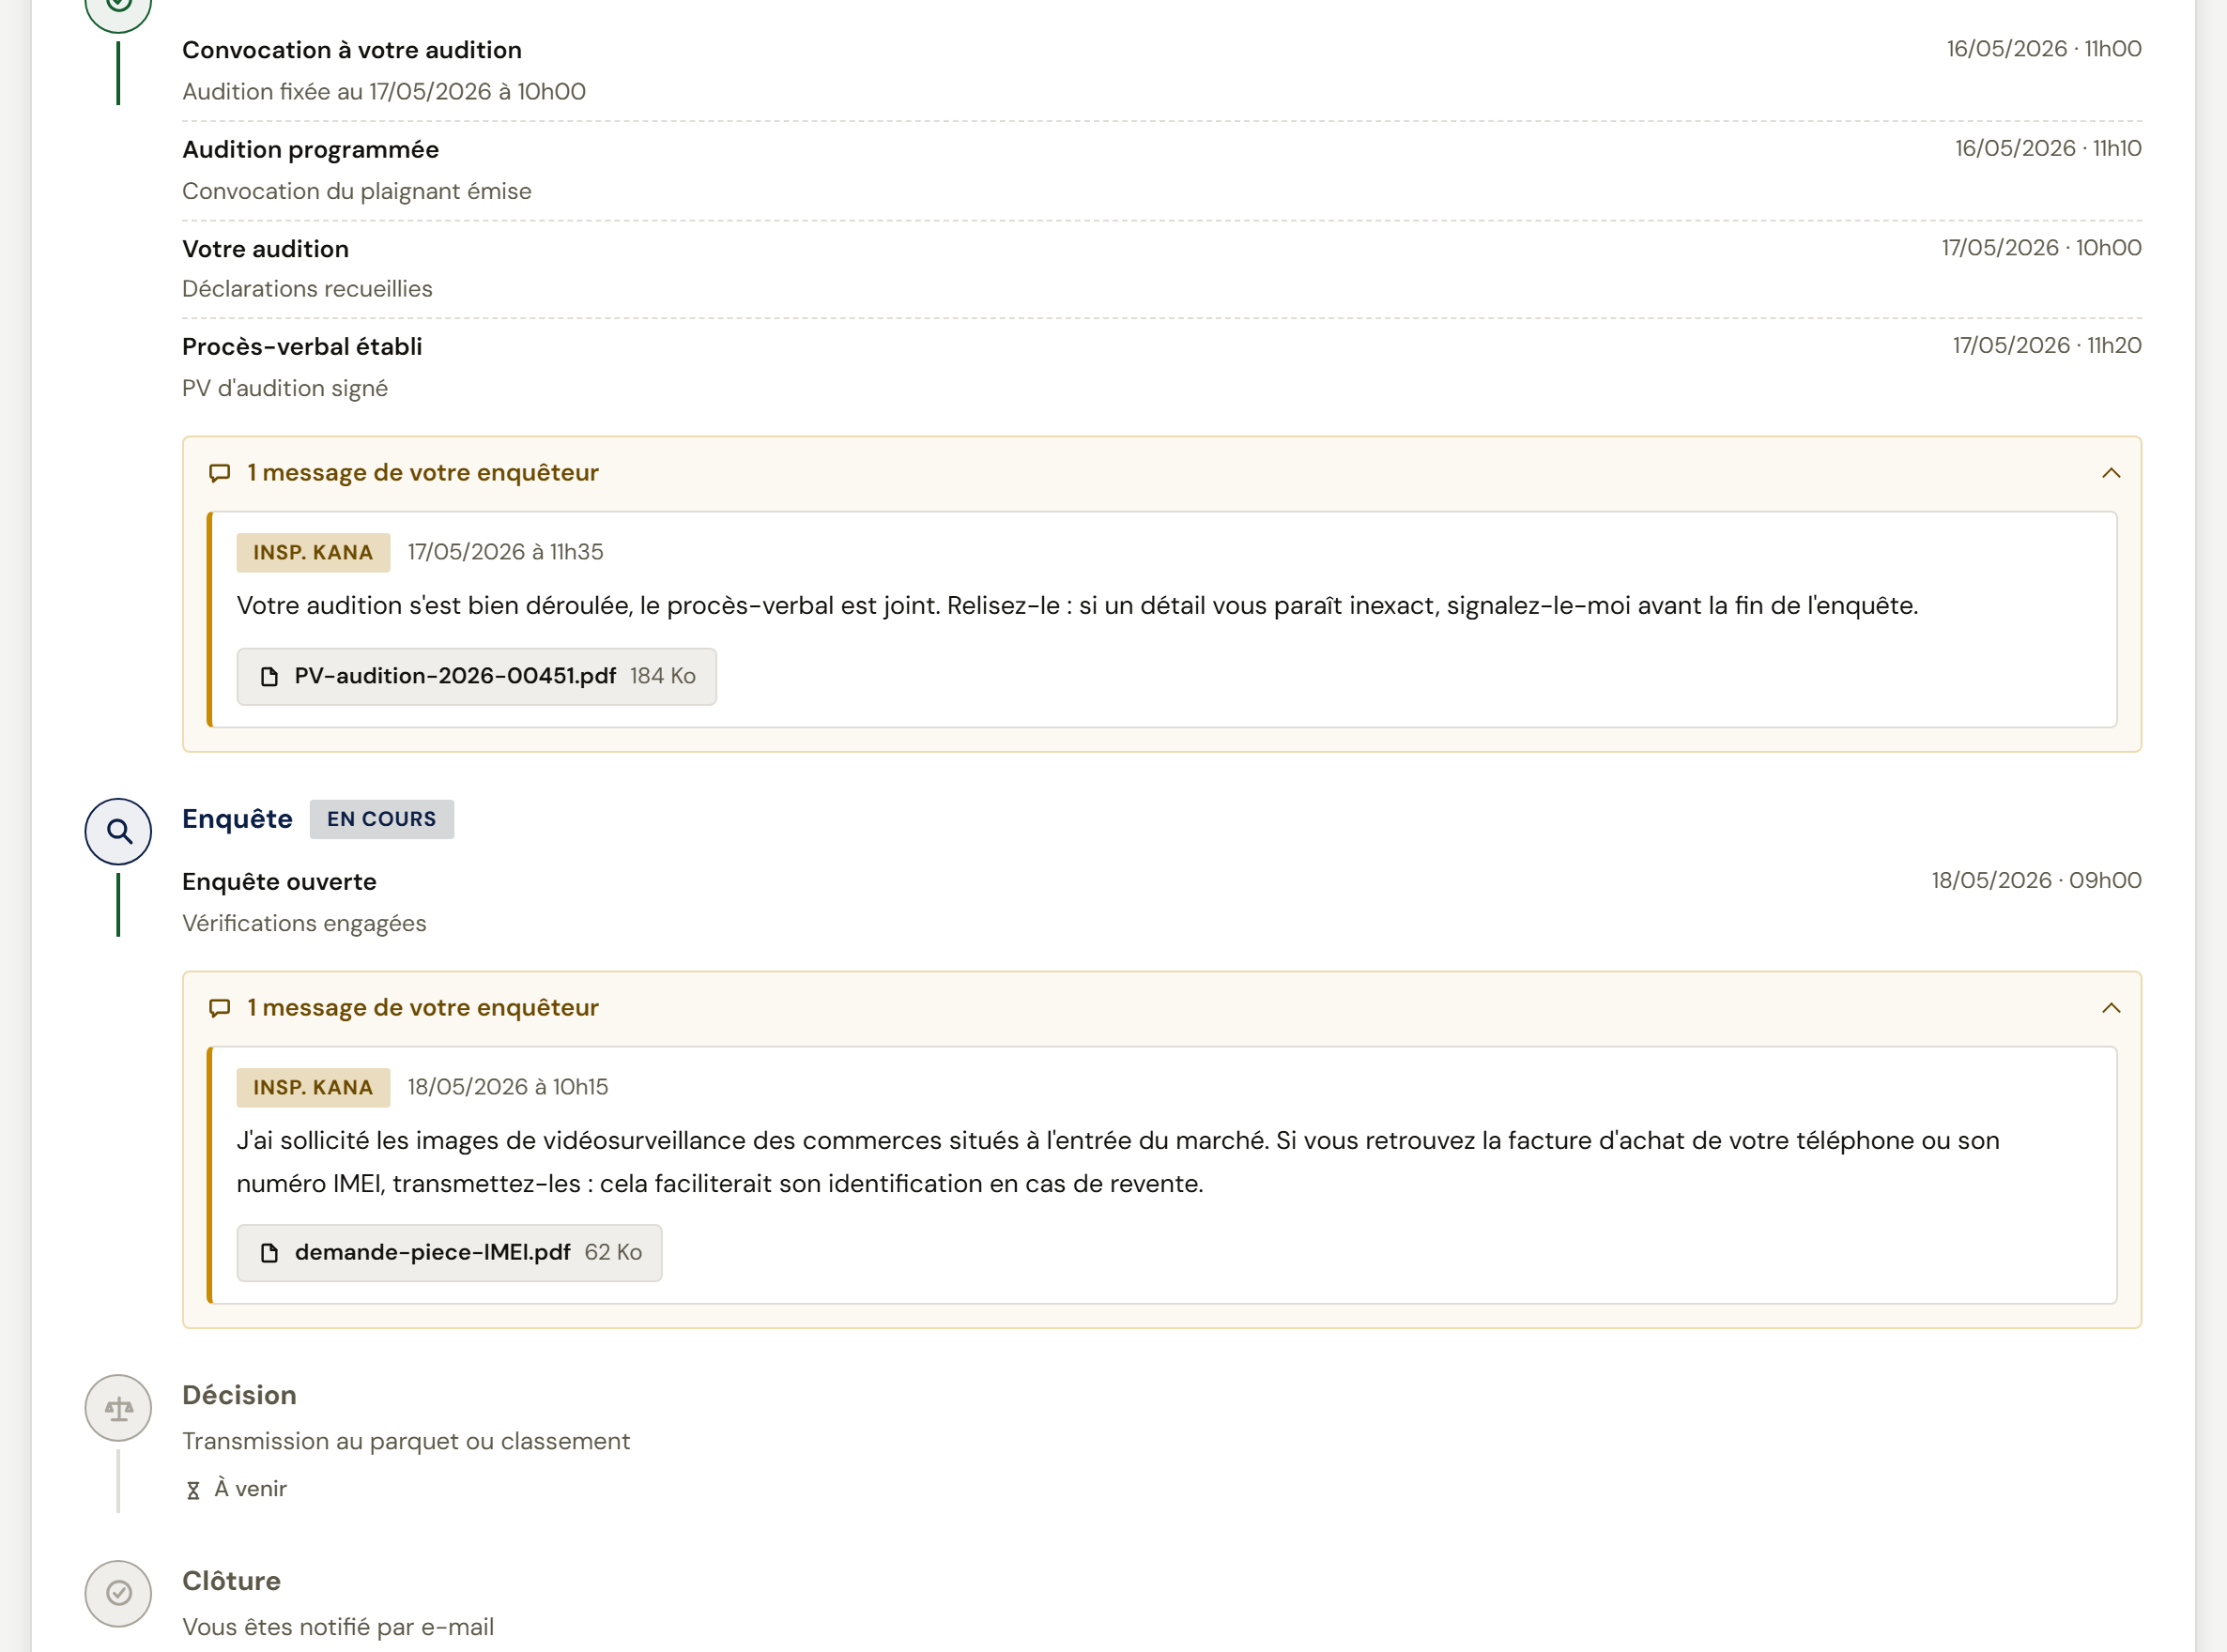
\includegraphics[width=0.58\textwidth]{images/notification.png}
    \caption{Centre de notifications}
    \label{fig:notifications}
\end{figure}

Changement de statut, convocation émise ou demande de pièce complémentaire : chaque notification porte un lien direct vers le dossier concerné. Le plaignant est informé de l'avancement de sa procédure sans se déplacer ni téléphoner au commissariat (BF6).

\subsection{Historique et traçabilité}

\begin{figure}[H]
    \centering
    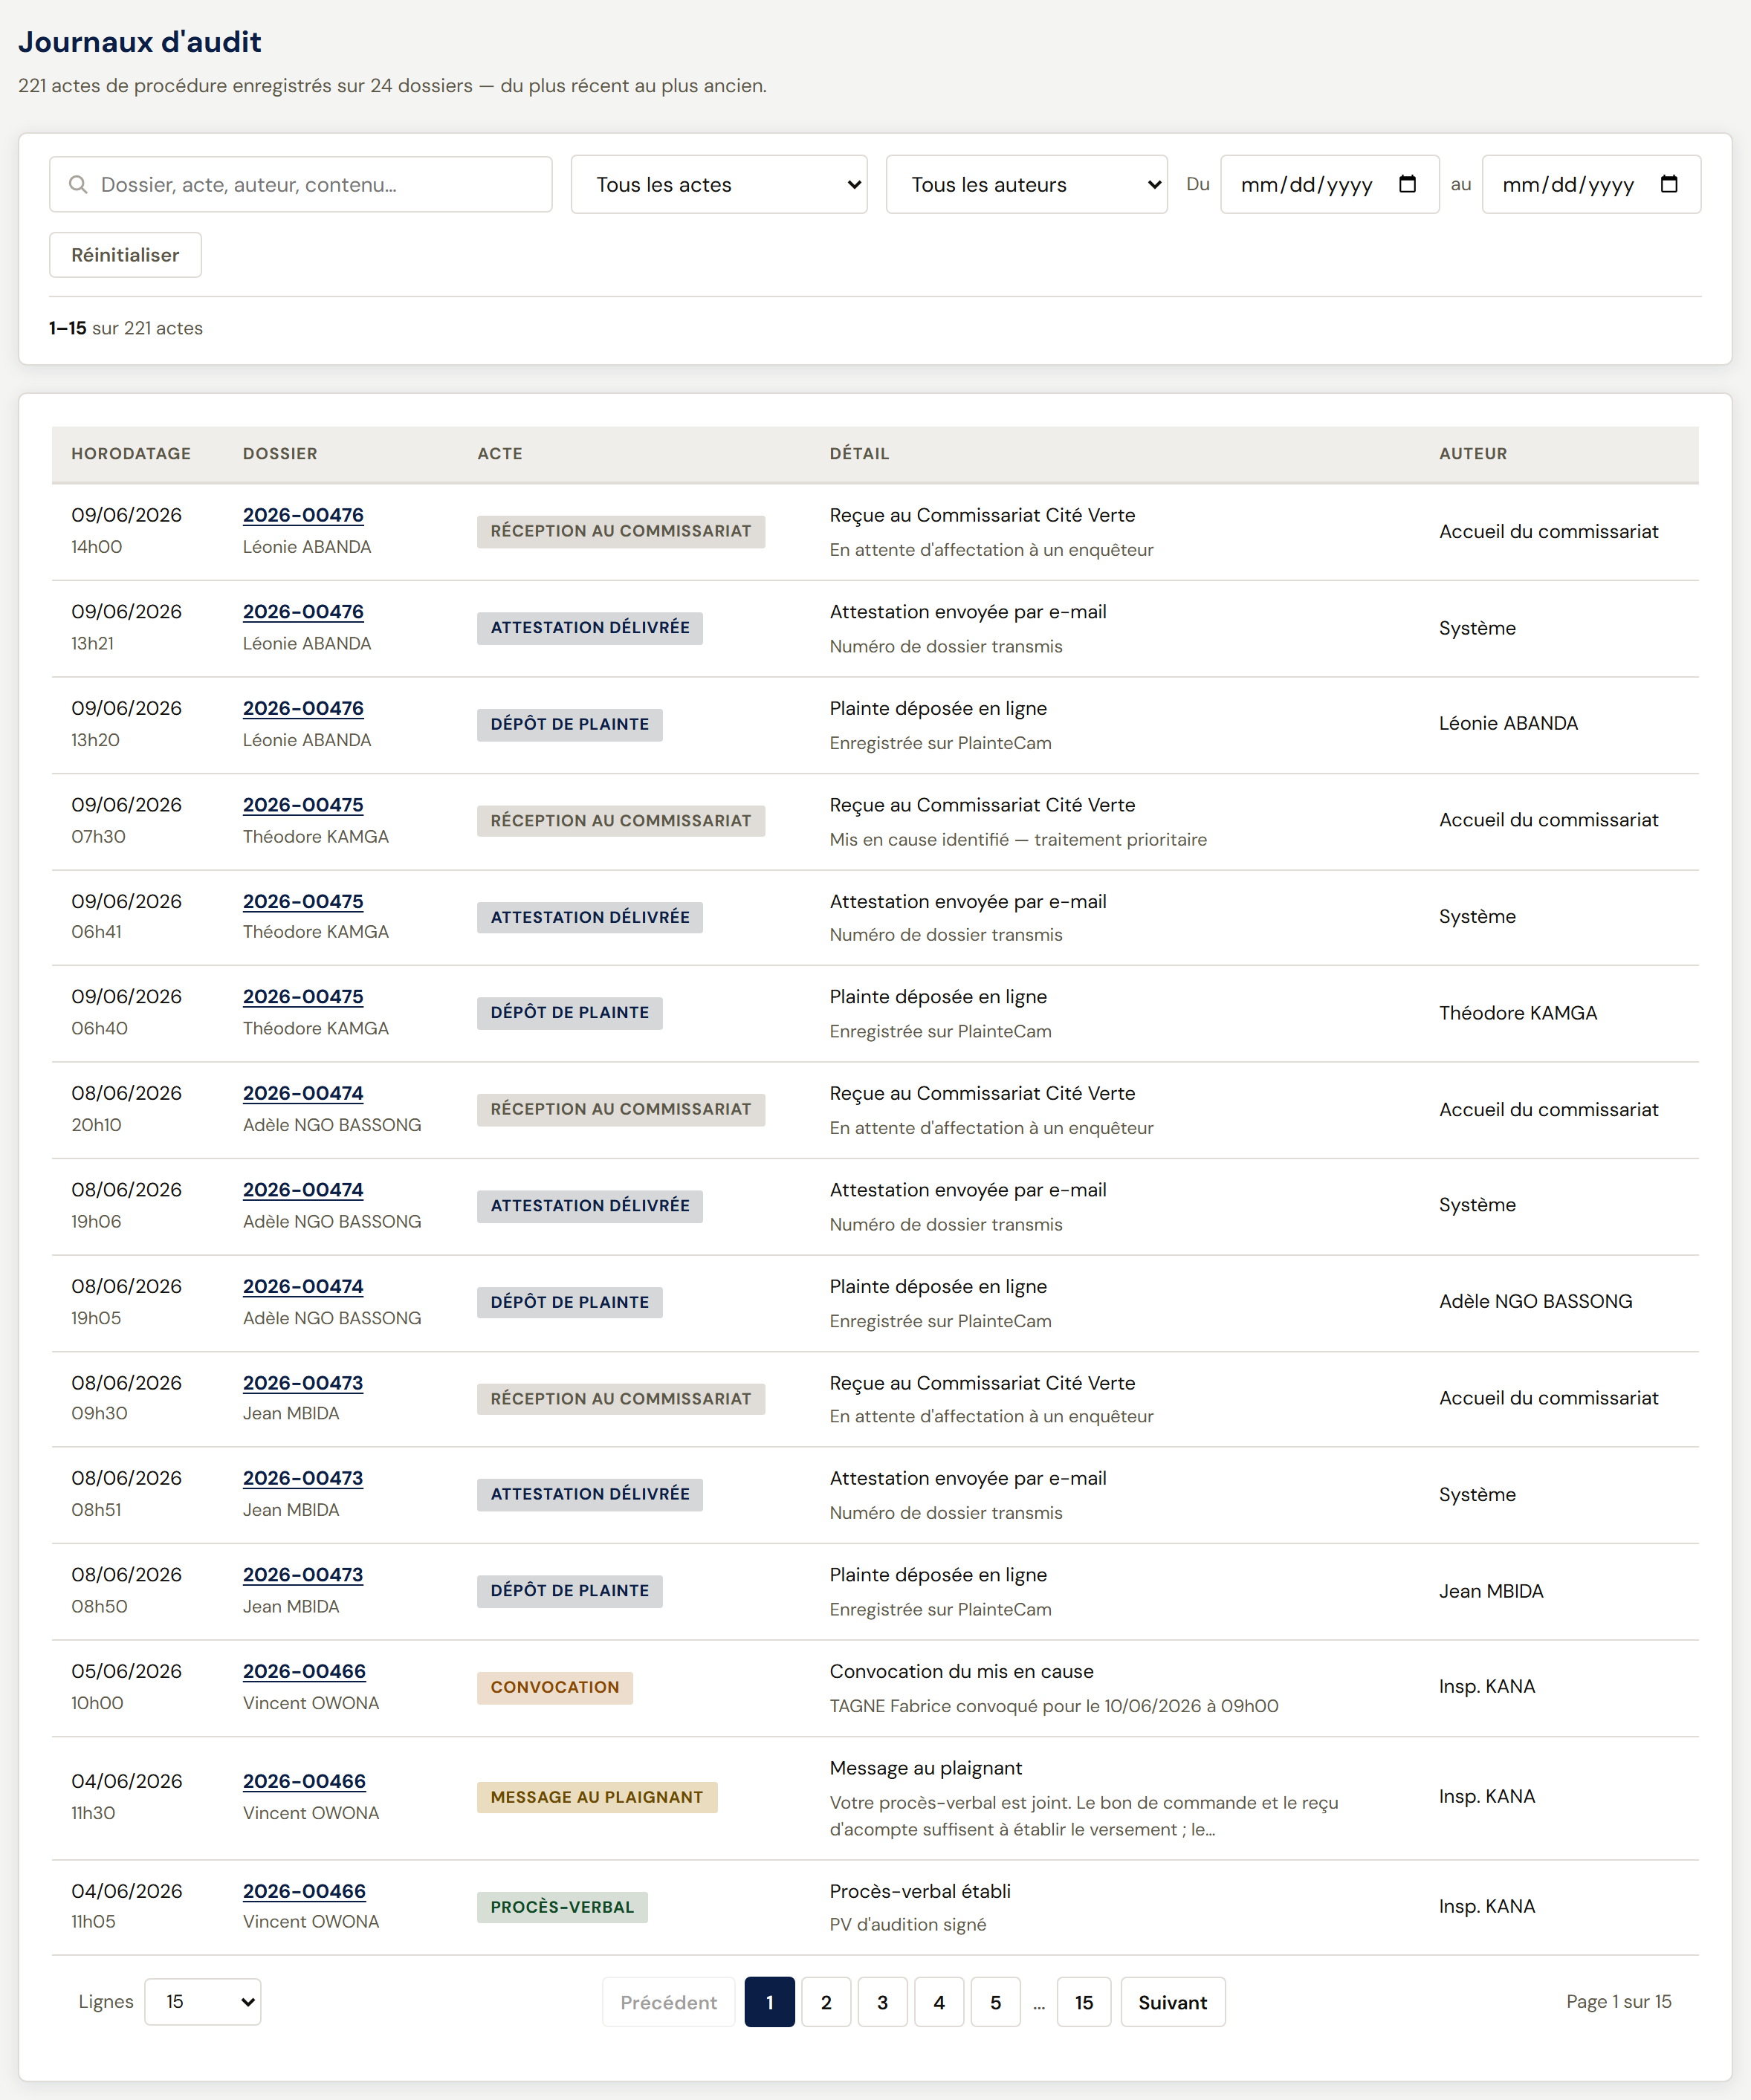
\includegraphics[width=0.58\textwidth]{images/historique.png}
    \caption{Journal d'audit, traçabilité de la procédure}
    \label{fig:historique}
\end{figure}

Chaque transition de statut, cotation, audition et validation de procès-verbal est horodatée et rattachée à son auteur. Ce journal constitue la contrepartie numérique du registre de main courante et fonde autant la conformité que le pilotage (BNF2).

\subsection{Statistiques et pilotage}

\begin{figure}[H]
    \centering
    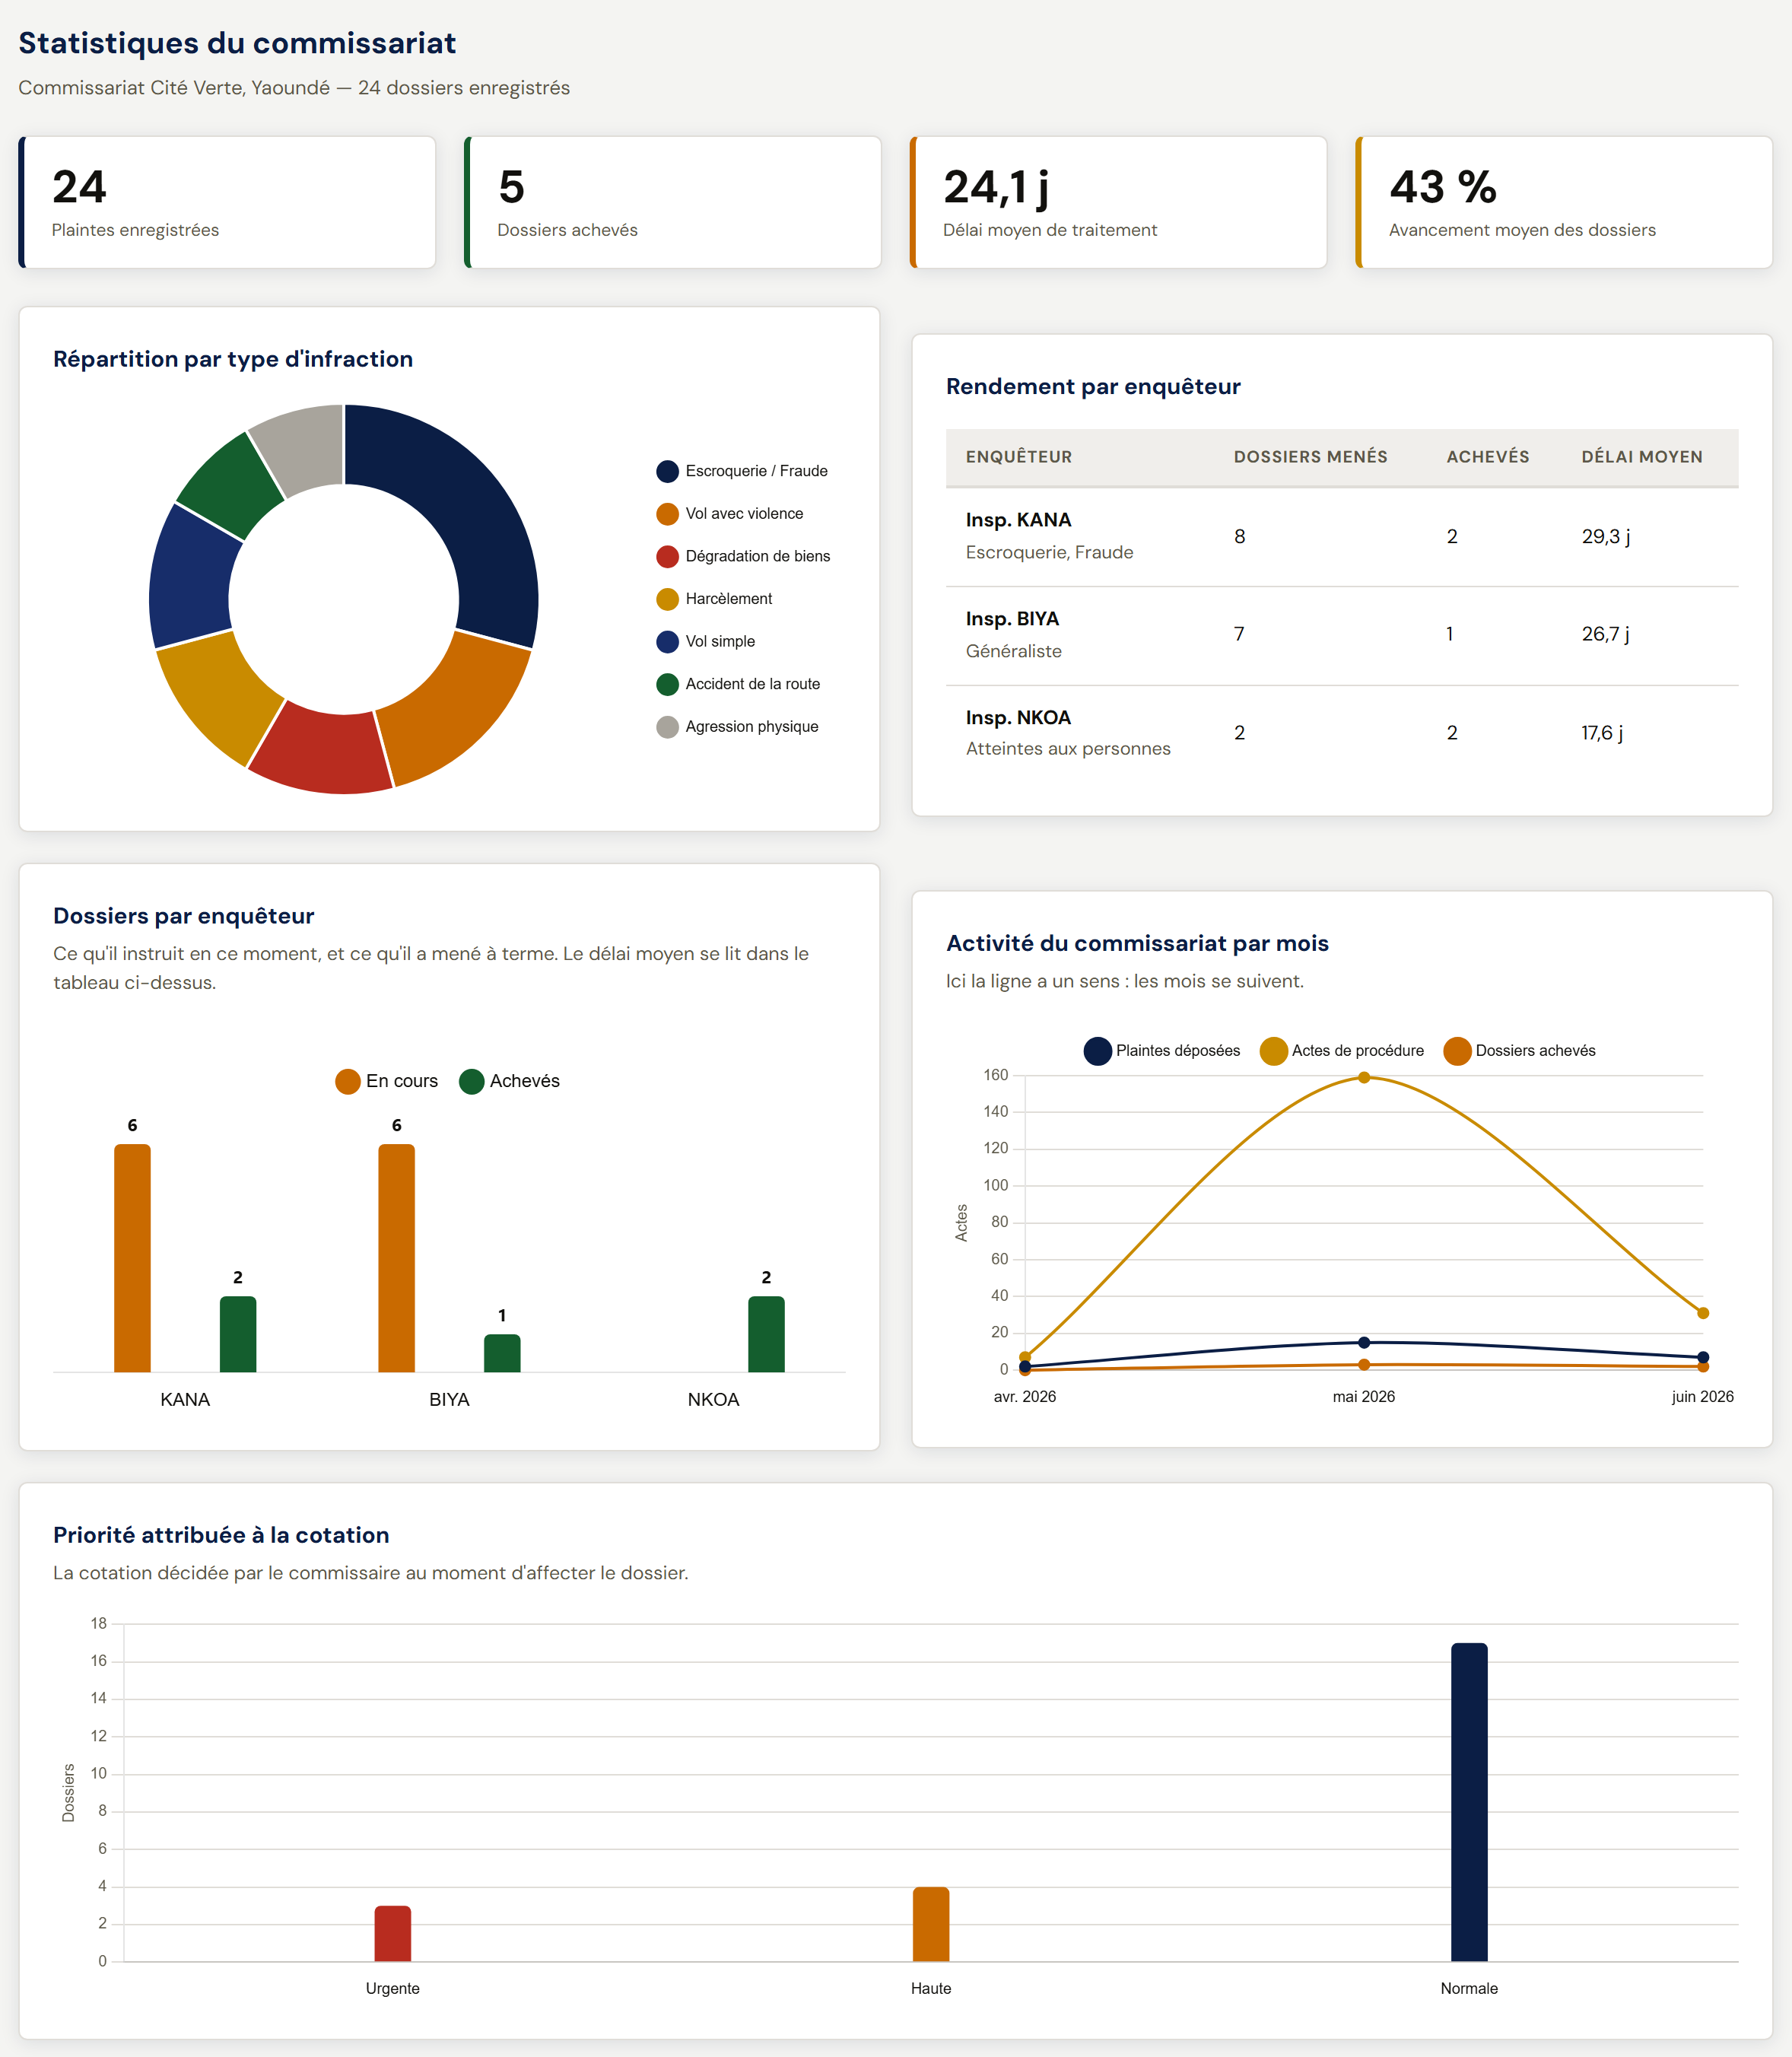
\includegraphics[width=0.58\textwidth]{images/avancee.png}
    \caption{Module de statistiques, répartitions et indicateurs}
    \label{fig:analyse}
\end{figure}

Répartition des plaintes par statut, par nature d'infraction et par priorité, charge par enquêteur : le commissaire dispose d'indicateurs objectifs pour répartir le travail et identifier les infractions dominantes sur son ressort.
        % Chapitre 3
% CONCLUSION GÉNÉRALE (2 pages)

\chapter*{CONCLUSION GÉNÉRALE}
\addcontentsline{toc}{chapter}{Conclusion Générale}
\label{ch:conclusion}

\section*{Synthèse des missions}
\addcontentsline{toc}{section}{Synthèse des missions}

Ce stage de six mois au sein de \textbf{KLIVAR} avait pour objectif de répondre à un défi concret : dématérialiser le dépôt et le traitement des plaintes citoyennes, qui reposaient jusqu'alors entièrement sur des échanges physiques et des pièces papier.

La solution développée, \textbf{PlainteCam}, est une plateforme web full-stack intégrant un frontend React.js, un backend Flask exposant une API REST, et le modèle génératif Llama 3.1 servi par la plateforme d'inférence Groq. Elle couvre l'ensemble du cycle de vie d'un dossier : dépôt guidé par le citoyen, rattachement automatique au commissariat compétent, cotation de l'enquête par le commissaire, rédaction assistée du procès-verbal par l'enquêteur, convocation, suivi en ligne par le plaignant et clôture.

Les objectifs fixés au départ ont été atteints sur le périmètre de la recette :

\begin{itemize}
    \item Suppression du déplacement obligatoire pour porter plainte
    \item Rattachement automatique du dossier au commissariat territorialement compétent dès la saisie du lieu des faits, sans circulation de pièces papier
    \item Procès-verbal proposé en moins de deux minutes, puis révisé et validé par l'enquêteur
    \item Traçabilité horodatée de \textbf{100\%} des transitions de statut
    \item Suivi du dossier accessible en ligne au plaignant
\end{itemize}

La confirmation de ces gains en exploitation réelle suppose toutefois un déploiement instrumenté, tel que recommandé au chapitre~\ref{ch:bilan}.

\section*{Bilan personnel}
\addcontentsline{toc}{section}{Bilan personnel}

Cette expérience professionnelle a été enrichissante à plusieurs niveaux.

\textbf{Compétences techniques (hard skills) acquises :}
\begin{itemize}
    \item Développement full-stack React.js / Flask en contexte professionnel
    \item Intégration d'une API d'intelligence artificielle générative dans une application métier, et conception des garde-fous qui l'encadrent
    \item Conception et modélisation d'architectures logicielles (UML, REST, modèle relationnel)
    \item Sécurisation d'une API par jeton et cloisonnement des accès par rôle
    \item Mise en place d'une démarche Agile Scrum avec livraisons itératives
\end{itemize}

\textbf{Compétences transversales (soft skills) développées :}
\begin{itemize}
    \item Capacité à reformuler un besoin métier réglementé en exigences techniques claires
    \item Conduite d'entretiens terrain avec des personnels de commissariat et restitution des constats
    \item Gestion de projet en autonomie avec reporting régulier au maître de stage
    \item Adaptabilité face aux imprévus et aux changements de priorité en cours de projet
    \item Esprit de synthèse pour la documentation et la rédaction du présent mémoire
\end{itemize}

\section*{Perspectives d'évolution}
\addcontentsline{toc}{section}{Perspectives d'évolution}

PlainteCam, dans sa version actuelle, constitue une base opérationnelle. Plusieurs axes d'évolution ont été identifiés pour la suite du projet :

\textbf{À court terme :} Instrumentation des indicateurs, test de charge, puis déploiement sur un commissariat pilote avec formation des personnels et dispositif de support.

\textbf{À moyen terme :} Transcription vocale côté serveur, afin d'affranchir la dictée des limites du navigateur et d'ouvrir la voie au traitement des langues nationales. Ajout de la géolocalisation du lieu des faits pour affiner le rattachement territorial.

\textbf{À long terme :} Analyse des données consolidées pour identifier les zones et les périodes de forte sinistralité et adapter l'allocation des effectifs. Interconnexion avec les systèmes d'information judiciaires pour la transmission dématérialisée des dossiers au parquet.

\medskip

En définitive, cette mission a montré qu'une technologie bien choisie peut transformer une procédure administrative lourde en un parcours lisible pour le citoyen, sans rien retirer aux garanties qui l'entourent. Elle a aussi rappelé qu'en matière régalienne, la valeur d'une plateforme se juge autant à la confiance qu'elle inspire qu'aux minutes qu'elle fait gagner. C'est cette double exigence qui a guidé l'ensemble du travail réalisé durant ce stage.


% ── POSTLIMINAIRES ───────────────────────────────────────────
\appendix
% ANNEXES

\chapter{Annexes}
\label{ch:annexes}

\section*{Annexe A — Manuel utilisateur (extrait)}

\subsection*{A.1 — Déposer une plainte (espace citoyen)}

\begin{enumerate}
    \item Se connecter à l'espace citoyen avec son adresse électronique. Un code à usage unique est envoyé par courriel ; il est valable dix minutes.
    \item Choisir \textbf{Déposer une plainte}, puis la \textbf{nature de l'infraction} dans la liste proposée.
    \item Renseigner le lieu des faits par la cascade \textbf{Région $\rightarrow$ Département $\rightarrow$ Arrondissement $\rightarrow$ Quartier}. Le commissariat compétent s'affiche automatiquement.
    \item Rédiger le \textbf{récit des faits}. Le bouton microphone permet de dicter la déclaration plutôt que de la saisir.
    \item Indiquer l'\textbf{identité du mis en cause} si elle est connue ; cette étape peut être passée.
    \item Répondre aux \textbf{questions complémentaires} propres à la nature déclarée. Les questions déjà couvertes par le récit ne sont pas posées.
    \item Vérifier l'\textbf{aperçu}, signer, puis valider. Le \textbf{récépissé} au format PDF, portant le numéro de dossier et un QR code de vérification, est téléchargeable immédiatement.
\end{enumerate}

\figopt{ecran_depot_nature.png}{0.58}{Étape 1 — nature de l'infraction et cascade de localisation}{fig:man_depot_nature}

\figopt{ecran_depot_apercu.png}{0.58}{Étape 5 — aperçu de la déclaration avant signature}{fig:man_depot_apercu}

\subsection*{A.2 — Suivre son dossier}

Depuis \textbf{Mes plaintes}, le plaignant consulte l'état de chacun de ses dossiers. Les statuts successifs sont : \textit{Reçu}, \textit{Audition}, \textit{En instruction}, \textit{Décision}, \textit{Transmis}, \textit{Clôturé}. Toute convocation reçue apparaît dans le dossier concerné.

\figopt{ecran_suivi.png}{0.58}{Espace citoyen — suivi de l'avancement d'un dossier}{fig:man_suivi}

\subsection*{A.3 — Coter un dossier (espace commissaire)}

Depuis le tableau de bord, sélectionner un dossier au statut \textit{Reçu}, cliquer sur \textbf{Coter}, désigner l'enquêteur destinataire et confirmer la priorité proposée. La cotation est inscrite au journal d'audit et notifiée à l'enquêteur.

\figopt{ecran_cotation.png}{0.58}{Espace commissaire — cotation d'un dossier à un enquêteur}{fig:man_cotation}

\subsection*{A.4 — Dresser un procès-verbal (espace enquêteur)}

Ouvrir un dossier coté, puis choisir \textbf{Nouveau PV} et sélectionner l'audition concernée. Une proposition rédigée à partir de la déclaration s'affiche dans l'éditeur. \textbf{La relecture est obligatoire} : corriger, compléter, puis valider et signer. Le PV n'est enregistré qu'après validation explicite.

\figopt{ecran_pv.png}{0.58}{Espace enquêteur — éditeur de procès-verbal, proposition révisable}{fig:man_pv}

\section*{Annexe B — Captures d'écran complémentaires}

\figopt{ecran_connexion.png}{0.58}{Écran de connexion — choix du rôle et authentification}{fig:cap_connexion}

\figopt{ecran_recepisse.png}{0.58}{Récépissé de dépôt de plainte généré au format PDF}{fig:cap_recepisse}

\figopt{ecran_convocation.png}{0.58}{Convocation émise par l'enquêteur}{fig:cap_convocation}

\figopt{ecran_qr.png}{0.58}{Vérification d'une pièce par son QR code}{fig:cap_qr}

\section*{Annexe C — Extraits de code}

\subsection*{C.1 — Dépôt d'une plainte et rattachement au commissariat}

\begin{lstlisting}[language=Python,caption={Endpoint Flask de dépôt d'une plainte},label={lst:depot}]
@app.route("/api/plaintes", methods=["POST"])
@jwt_required()
def deposer_plainte():
    """Enregistre une plainte et la rattache au commissariat competent."""
    donnees = PlainteSchema().load(request.get_json())
    citoyen_id = get_jwt_identity()

    # Le ressort territorial determine le commissariat : le quartier
    # des faits, et non le domicile du plaignant, fait autorite.
    commissariat = Commissariat.query.filter_by(
        quartier=donnees["quartier"]
    ).first_or_404(description="Aucun commissariat pour ce quartier")

    plainte = Plainte(
        citoyen_id=citoyen_id,
        commissariat_id=commissariat.id,
        nature=donnees["nature"],
        recit=donnees["recit"],
        statut=StatutPlainte.RECU,
        score_completude=calculer_score(donnees),
    )
    db.session.add(plainte)
    db.session.flush()          # obtient l'id avant l'ecriture du journal

    journaliser(plainte.id, "DEPOT", auteur=citoyen_id)
    db.session.commit()

    return jsonify(PlainteSchema().dump(plainte)), 201
\end{lstlisting}

\subsection*{C.2 — Rédaction assistée du procès-verbal}

\begin{lstlisting}[language=Python,caption={Appel au modèle génératif (Llama 3.1 via Groq), côté serveur},label={lst:ia}]
from groq import Groq

client = Groq(api_key=os.environ["GROQ_API_KEY"])   # jamais en dur

def proposer_proces_verbal(plainte):
    """Retourne une PROPOSITION de PV. La validation par l'enqueteur
    reste obligatoire : cette fonction n'ecrit rien en base."""
    consigne = (
        "Tu rediges un projet de proces-verbal d'audition a partir de la "
        "declaration ci-dessous. Style administratif, troisieme personne. "
        "N'invente aucun fait absent de la declaration : en cas de donnee "
        "manquante, ecris [A COMPLETER PAR L'ENQUETEUR]."
    )
    reponse = client.chat.completions.create(
        model="llama-3.1-8b-instant",
        messages=[
            {"role": "system",  "content": consigne},
            {"role": "user",    "content": f"Nature : {plainte.nature}\n"
                                           f"Declaration : {plainte.recit}"},
        ],
        temperature=0.2,        # bas : on veut de la fidelite, pas du style
    )
    return reponse.choices[0].message.content
\end{lstlisting}

\subsection*{C.3 — Cloisonnement des accès au niveau du SGBD}

\begin{lstlisting}[language=SQL,caption={Politique d'accès par ligne sur la table des plaintes},label={lst:rls}]
-- Un plaignant ne voit que ses propres dossiers.
CREATE POLICY plaintes_select_citoyen ON plaintes
  FOR SELECT USING (citoyen_id = current_user_id());

-- Un enqueteur ne voit que les dossiers qui lui ont ete cotes.
CREATE POLICY plaintes_select_enqueteur ON plaintes
  FOR SELECT USING (enqueteur_id = current_user_id());

-- Un commissaire voit tous les dossiers de son commissariat.
CREATE POLICY plaintes_select_commissaire ON plaintes
  FOR SELECT USING (commissariat_id = current_user_commissariat());
\end{lstlisting}

\section*{Annexe D — Fiches de tests}

\begin{table}[H]
    \centering
    \begin{tabularx}{\textwidth}{|l|>{\raggedright\arraybackslash}X|>{\raggedright\arraybackslash}X|l|}
        \hline
        \textbf{Réf.} & \textbf{Cas de test} & \textbf{Résultat attendu} & \textbf{Verdict} \\
        \hline
        T-01 & Dépôt d'une plainte pour vol simple, les 5 étapes renseignées & Dossier créé au statut \textit{Reçu}, récépissé PDF délivré & Conforme \\
        \hline
        T-02 & Dépôt avec identité du mis en cause laissée vide & Dépôt accepté, champ marqué « inconnu » & Conforme \\
        \hline
        T-03 & Sélection d'un quartier hors ressort couvert & Message d'erreur explicite, dépôt bloqué & Conforme \\
        \hline
        T-04 & Récit mentionnant déjà l'heure et les témoins & Questions correspondantes non posées & Conforme \\
        \hline
        T-05 & Cotation d'un dossier à un enquêteur, priorité \textit{Haute} & Dossier visible chez l'enquêteur, cotation journalisée & Conforme \\
        \hline
        T-06 & Consultation par un citoyen du dossier d'un tiers & Accès refusé & Refusé comme attendu \\
        \hline
        T-07 & Appel de l'API sans jeton d'authentification & Réponse HTTP 401 & Refusé comme attendu \\
        \hline
        T-08 & Proposition de PV puis validation sans relecture & Validation possible mais tracée au nom de l'enquêteur & Conforme, point de vigilance \\
        \hline
        T-09 & Vérification du QR code d'un récépissé & Renvoi vers le dossier correspondant & Conforme \\
        \hline
        T-10 & Déclaration dictée puis relue à l'écran & Texte transcrit, corrections manuelles nécessaires & Conforme, limite connue \\
        \hline
    \end{tabularx}
    \caption{Fiches de tests de recette}
    \label{tab:fiches_tests}
\end{table}

\section*{Annexe E — Glossaire technique}

\begin{table}[H]
    \centering
    \begin{tabularx}{\textwidth}{|l|X|}
        \hline
        \textbf{Terme} & \textbf{Définition} \\
        \hline
        API REST & Interface de programmation suivant le style architectural REST, permettant au frontend et au backend de communiquer par requêtes HTTP standardisées. \\
        \hline
        Cotation & Acte par lequel le commissaire désigne l'enquêteur chargé d'une affaire et en fixe la priorité. \\
        \hline
        Procès-verbal (PV) & Acte écrit par lequel un officier de police judiciaire consigne des déclarations ou des constatations. \\
        \hline
        Récépissé & Document remis au plaignant attestant du dépôt de sa plainte et portant le numéro de dossier. \\
        \hline
        IA générative & Système capable de produire un texte structuré à partir d'une entrée en langage naturel. Dans PlainteCam, elle ne produit que des propositions soumises à validation. \\
        \hline
        Architecture trois-tiers & Modèle séparant la présentation (frontend), la logique métier (backend) et la persistance (base de données). \\
        \hline
        Jeton JWT & Jeton signé transmis à chaque requête pour vérifier l'identité et le rôle de l'appelant, sans session côté serveur. \\
        \hline
        ORM & Technique de mapping objet-relationnel permettant de manipuler la base via des objets Python plutôt que par du SQL écrit à la main. \\
        \hline
        WSGI & Interface standard entre un serveur web et une application Python, définie par la PEP 3333. \\
        \hline
        Politique d'accès par ligne & Règle appliquée par le SGBD lui-même, restreignant les lignes visibles selon l'utilisateur connecté. \\
        \hline
        Agile Scrum & Cadre de gestion de projet itératif organisant le développement en sprints de durée fixe. \\
        \hline
    \end{tabularx}
    \caption{Glossaire des termes techniques et métier}
    \label{tab:glossaire}
\end{table}

\cleardoublepage
\phantomsection
\addcontentsline{toc}{chapter}{Bibliographie}
\bibliographystyle{plain}
\bibliography{bibli}
\end{document}
